\documentclass[10pt,a4paper,twoside,openany,parskip=half]{scrbook}

\usepackage[utf8]{inputenc}
\usepackage[T1]{fontenc}
\usepackage{amsmath,amsthm,mathtools}
\usepackage[lining,semibold]{libertine}
\usepackage[scaled=0.85]{beramono}
\let\openbox\relax
\let\Bbbk\relax
\usepackage[libertine,vvarbb]{newtxmath}
\let\Bbbk\relax
\usepackage{amssymb}
\usepackage[english]{babel}
\usepackage{microtype}
\usepackage{graphicx}
\usepackage{array}
\usepackage{tikz}
\usepackage{tikz-cd}
\usepackage[inline]{enumitem}
\usepackage{multicol}
\setlength{\multicolsep}{4pt plus 2pt}
\setlist{itemsep=2pt,parsep=2pt,topsep=4pt}
\usepackage{xcolor}
\usepackage[most]{tcolorbox}
\usepackage[a4paper,inner=28mm,outer=24mm,top=24mm,bottom=26mm,headsep=8mm,footskip=14mm]{geometry}
\usepackage{scrlayer-scrpage}
\pagestyle{scrheadings}
\automark[section]{chapter}
\clearpairofpagestyles
\ihead{\textsc{\leftmark}}
\ohead{\textsc{\rightmark}}
\ofoot[\pagemark]{\pagemark}

\usepackage[colorlinks=true,linkcolor=teal!55!black,urlcolor=teal!55!black,citecolor=teal!55!black,bookmarksnumbered=true,bookmarksopen=true,pdftitle={Linear Algebra},pdfauthor={Tomasz Brengos}]{hyperref}

% --- Palette ---
\definecolor{defaccent}{HTML}{1F4E79}
\definecolor{thmaccent}{HTML}{6A1B9A}
\definecolor{exaccent}{HTML}{2E7D32}
\definecolor{remaccent}{HTML}{546E7A}
\definecolor{warnaccent}{HTML}{D84315}
\definecolor{exercaccent}{HTML}{D84315}
\definecolor{titleaccent}{HTML}{1F4E79}

% --- Chapter & section appearance ---
\setkomafont{disposition}{\normalfont\sffamily\bfseries}
\setkomafont{chapter}{\Huge\sffamily\bfseries\color{titleaccent}}
\setkomafont{chapterprefix}{\Large\sffamily\mdseries\color{remaccent}}
\setkomafont{section}{\Large\sffamily\bfseries\color{titleaccent!90!black}}
\setkomafont{subsection}{\large\sffamily\bfseries}
\renewcommand*{\chapterformat}{\textcolor{remaccent}{\thechapter}\enskip}
\renewcommand*{\raggedchapter}{\raggedright}

% --- Theorem environments ---
\theoremstyle{definition}
\newtheorem{definition}{Definition}[chapter]
\newtheorem{example}[definition]{Example}
\newtheorem{remark}[definition]{Remark}
\newtheorem{fact}[definition]{Fact}
\newtheorem{observation}[definition]{Observation}
\theoremstyle{plain}
\newtheorem{theorem}[definition]{Theorem}
\newtheorem{lemma}[definition]{Lemma}
\newtheorem{corollary}[definition]{Corollary}
\newtheorem{proposition}[definition]{Proposition}

% A lightweight "warning" environment (for cautions / common mistakes)
\theoremstyle{remark}
\newtheorem*{warning}{Warning}

% Exercises (collected in the final chapter)
\theoremstyle{definition}
\newtheorem{exercise}{Exercise}[section]

% Common box style: left accent bar, no surrounding frame, breakable
\tcolorboxenvironment{definition}{
  blanker, breakable,
  before skip=10pt, after skip=10pt,
  borderline west={2.5pt}{0pt}{defaccent},
  left=10pt, top=2pt, bottom=2pt
}
\tcolorboxenvironment{theorem}{
  blanker, breakable,
  before skip=10pt, after skip=10pt,
  borderline west={2.5pt}{0pt}{thmaccent},
  left=10pt, top=2pt, bottom=2pt
}
\tcolorboxenvironment{lemma}{
  blanker, breakable,
  before skip=10pt, after skip=10pt,
  borderline west={2.5pt}{0pt}{thmaccent},
  left=10pt, top=2pt, bottom=2pt
}
\tcolorboxenvironment{corollary}{
  blanker, breakable,
  before skip=10pt, after skip=10pt,
  borderline west={2.5pt}{0pt}{thmaccent},
  left=10pt, top=2pt, bottom=2pt
}
\tcolorboxenvironment{proposition}{
  blanker, breakable,
  before skip=10pt, after skip=10pt,
  borderline west={2.5pt}{0pt}{thmaccent},
  left=10pt, top=2pt, bottom=2pt
}
\tcolorboxenvironment{example}{
  blanker, breakable,
  before skip=10pt, after skip=10pt,
  borderline west={2.5pt}{0pt}{exaccent},
  left=10pt, top=2pt, bottom=2pt
}
\tcolorboxenvironment{remark}{
  blanker, breakable,
  before skip=8pt, after skip=8pt,
  borderline west={1.8pt}{0pt}{remaccent},
  left=8pt, top=2pt, bottom=2pt
}
\tcolorboxenvironment{fact}{
  blanker, breakable,
  before skip=8pt, after skip=8pt,
  borderline west={1.8pt}{0pt}{remaccent},
  left=8pt, top=2pt, bottom=2pt
}
\tcolorboxenvironment{observation}{
  blanker, breakable,
  before skip=8pt, after skip=8pt,
  borderline west={1.8pt}{0pt}{remaccent},
  left=8pt, top=2pt, bottom=2pt
}
\tcolorboxenvironment{warning}{
  blanker, breakable,
  before skip=10pt, after skip=10pt,
  borderline west={2.5pt}{0pt}{warnaccent},
  left=10pt, top=2pt, bottom=2pt
}
\tcolorboxenvironment{exercise}{
  blanker, breakable,
  before skip=10pt, after skip=10pt,
  borderline west={2.5pt}{0pt}{exercaccent},
  left=10pt, top=2pt, bottom=2pt
}

% --- Math macros ---
\newcommand{\K}{\mathbb{K}}
\newcommand{\R}{\mathbb{R}}
\let\C\relax
\newcommand{\C}{\mathbb{C}}
\let\N\relax
\newcommand{\N}{\mathbb{N}}
\newcommand{\Q}{\mathbb{Q}}
\let\Z\relax
\newcommand{\Z}{\mathbb{Z}}
\let\V\relax
\newcommand{\V}{\mathbf{V}}
\let\W\relax
\newcommand{\W}{\mathbf{W}}
\let\vv\relax
\newcommand{\vv}{\mathbf{v}}
\let\uu\relax
\newcommand{\uu}{\mathbf{u}}
\let\ww\relax
\newcommand{\ww}{\mathbf{w}}
\newcommand{\0}{\mathbf{0}}
\DeclareMathOperator{\spanop}{span}
\newcommand{\Span}[1]{\operatorname{span}\!\left(#1\right)}
\DeclareMathOperator{\rank}{r}
\renewcommand{\Re}{\mathfrak{Re}}
\renewcommand{\Im}{\mathfrak{Im}}
\let\det\relax
\DeclareMathOperator{\det}{det}

% --- Front matter metadata ---
\titlehead{\centering\sffamily\small Warsaw University of Technology}
\subject{\sffamily Lecture Notes}
\title{\sffamily\bfseries Linear Algebra}
\author{\sffamily Tomasz Brengos}
\date{}

\begin{document}
\frontmatter
\maketitle
\tableofcontents

\mainmatter

\chapter{Complex numbers}\label{ch:complex}
\section{Motivation}

The equation
\[
x^2+1=0
\]
has no real solutions, since $x^2\geq 0$ for every $x\in\R$. Nonetheless, we often need solutions of such
equations. The remedy is to \emph{extend} the set of real numbers: we introduce a new number
\[
i, \qquad \text{required to satisfy} \qquad i^2 = -1.
\]
Clearly $i$ is not a real number. As we shall see, adjoining $i$ to $\R$ produces a new field — the field of
complex numbers — in which \emph{every} polynomial equation has a solution.

So much for the algebra — but why should a computer scientist care about numbers that mathematicians
themselves long dismissed as ``imaginary''? Because complex numbers turned out to be one of the most
practical inventions in the history of mathematics. You have already used them today, probably several
times:

\begin{itemize}
\item \textbf{Multimedia and signal processing.} Every JPEG image, every MP3 file and every video call
relies on the \emph{Fast Fourier Transform} (FFT), an algorithm that decomposes a signal into a
combination of simple waves. The FFT is formulated entirely in terms of complex numbers — more precisely,
in terms of the \emph{roots of unity} that we compute at the end of this chapter. The reason your phone
can stream music in real time is that multiplying complex numbers of modulus $1$ is a very cheap way of
manipulating waves.
\item \textbf{Computer graphics and games.} As we shall see, multiplying by a complex number of modulus
$1$ \emph{rotates} the plane: rotating a 2D sprite is literally one complex multiplication. The same idea,
one dimension up, leads to \emph{quaternions} — a four-dimensional cousin of $\C$ used by every serious
game engine to rotate 3D objects smoothly and without the numerical artefacts of angle-based approaches.
\item \textbf{Quantum computing.} The state of a qubit is a pair of complex numbers, and everything a
quantum computer does is linear algebra over $\C$. The famous interference effects behind quantum speedups
are exactly additions of complex numbers with different arguments — the geometry of this chapter.
\item \textbf{Fractals.} The Mandelbrot set — perhaps the most famous computer-generated image in history —
is produced by iterating the map $z\mapsto z^2+c$ over complex numbers and colouring each pixel by how fast
the modulus $|z|$ escapes to infinity.
\end{itemize}

There is also an internal reason to start the course here. The complex numbers are the cleanest example of
a \emph{field} — the abstract structure, introduced in the next chapter, that provides the scalars for
everything that follows: vector spaces, matrices, determinants and eigenvalues. Moreover, some purely
real-looking problems of linear algebra secretly live in $\C$: in Chapter~\ref{ch:eigen} we will meet
perfectly ordinary real matrices whose eigenvalues simply do not exist over $\R$ and force us into the
complex plane whether we like it or not. Learning to compute in $\C$ now is a small investment with a
large payoff.

\section{The complex numbers}

\begin{definition}
A \emph{complex number} is an expression $a+bi$, where $a,b\in \R$. The set of all complex numbers is denoted
by $\C$.
\end{definition}

\begin{definition}
Addition and multiplication of complex numbers are defined by
\[
\begin{aligned}
(a+bi)+(c+di) &= (a+c) + (b+d)i,\\
(a+bi)\cdot(c+di) &= (ac-bd)+ (ad+bc)i.
\end{aligned}
\]
\end{definition}

\noindent The rule for multiplication is exactly what one obtains by expanding $(a+bi)(c+di)$ formally and
using $i^2=-1$.

\begin{example}
\[
(2+3i)+(1-2i) = 3+i, \qquad
(2+3i)\cdot(1-2i) = 2-4i+3i-6i^2 = 2-i+6 = 8-i.
\]
\end{example}

\begin{fact}
Addition and multiplication of complex numbers are both commutative and associative, and multiplication is
distributive over addition.
\end{fact}

\begin{proof}
A straightforward verification from the definitions.
\end{proof}

\begin{fact}[Inversion]
For any complex number $a+bi$ we have $(a+bi)(a-bi)=a^2+b^2$. Consequently, if $z=a+bi\neq 0$, then its
multiplicative inverse is
\[
\frac{1}{z}=\frac{1}{a+bi} = \frac{a}{a^2+b^2}-\frac{b}{a^2+b^2}\,i.
\]
\end{fact}

\begin{proof}
Multiplying numerator and denominator by the conjugate $a-bi$,
\[
\frac{1}{a+bi} =\frac{a-bi}{(a+bi)(a-bi)} = \frac{a-bi}{a^2+b^2}. \qedhere
\]
\end{proof}

\begin{example}
\[
\frac{1}{i} = \frac{-i}{i\cdot(-i)} = \frac{-i}{1} = -i, \qquad
\frac{1}{1+i} = \frac{1-i}{(1+i)(1-i)} = \frac{1-i}{2} =\tfrac12 + \tfrac12 i.
\]
\end{example}

\begin{theorem}
The set of complex numbers, with the addition and multiplication defined above, forms a field.
\end{theorem}

\noindent The general notion of a field is made precise in the next chapter; the theorem above says precisely
that $\C$ satisfies all of its axioms.

\section{Modulus, conjugate and the complex plane}

\begin{definition}
Let $z=a+bi$ be a complex number. We define
\[
\begin{aligned}
&\Re(z)=a && \text{(the \emph{real part} of $z$)},\\
&\Im(z)=b && \text{(the \emph{imaginary part} of $z$)},\\
&|z|=\sqrt{a^2+b^2} && \text{(the \emph{modulus} of $z$)},\\
&\bar{z}=a-bi && \text{(the \emph{conjugate} of $z$)}.
\end{aligned}
\]
\end{definition}

\begin{example}
For $z = 3-4i$ we have $\Re(z) = 3$, $\Im(z) = -4$ (note that the imaginary part is a \emph{real} number),
$|z| = \sqrt{9+16} = 5$ and $\bar z = 3+4i$. Moreover
$z\cdot\bar z = (3-4i)(3+4i) = 9+16 = 25 = |z|^2$.
\end{example}

\begin{fact}[Properties]
For complex numbers $z,z_1$,
\[
z\cdot \bar{z} = |z|^2, \qquad |z| = \sqrt{z\cdot \bar{z}}, \qquad
\Re(z) = \tfrac12 (z+\bar{z}), \qquad \Im(z) = \tfrac{1}{2i} (z-\bar{z}),
\]
and $|z-z_1|$ is the distance between the points $z$ and $z_1$.
\end{fact}

\begin{fact}[Algebra of conjugates and moduli]
For all $z,w\in\C$:
\[
\overline{z+w} = \bar z + \bar w, \qquad \overline{z\cdot w} = \bar z \cdot \bar w, \qquad \bar{\bar z} = z,
\qquad |z\cdot w| = |z|\,|w|, \qquad \left| \frac{z}{w} \right| = \frac{|z|}{|w|} \quad (w\neq 0).
\]
\end{fact}

\begin{example}[Geometric loci]
Since $|z-z_0|$ is the distance from $z$ to $z_0$, conditions on moduli describe geometric figures in the
complex plane:
\begin{itemize}
\item $\{z\in\C \mid |z-z_0| = r\}$ is the circle of radius $r$ centred at $z_0$; for instance
$|z+3-i| = 5$ describes the circle of radius $5$ centred at $z_0 = -3+i$ (note the signs:
$|z+3-i| = |z-(-3+i)|$).
\item $\{z\in\C \mid |z-z_0| \leq r\}$ is the closed disc of radius $r$ centred at $z_0$, and
$\{z\in\C \mid |z-z_0| > r\}$ is the exterior of that disc.
\item Conditions on $\Re$ and $\Im$ describe half-planes and lines: $\Re(z)>0$ is the open right
half-plane, while $\Im(z) = 1$ is a horizontal line.
\end{itemize}
\end{example}

Since a complex number $z=a+bi$ is a pair of real numbers, it can be drawn as a point (or vector) in the
plane — the \emph{complex plane} (or \emph{Argand diagram}). Its modulus $|z|$ is the length of the vector,
and its \emph{argument} $\varphi$ is the angle the vector makes with the positive real axis.

\begin{center}
\begin{tikzpicture}[scale=1.2,>=stealth]
  \draw[->] (-0.4,0) -- (3.2,0) node[right] {$\Re$};
  \draw[->] (0,-0.4) -- (0,2.6) node[above] {$\Im$};
  \coordinate (Z) at (2.4,2.0);
  \draw[->,thick,defaccent] (0,0) -- (Z) node[midway,above left] {$|z|$};
  \filldraw (Z) circle (1.2pt) node[right] {$z=a+bi$};
  \draw[dashed] (Z) -- (2.4,0) node[below] {$a$};
  \draw[dashed] (Z) -- (0,2.0) node[left] {$b$};
  \draw[exaccent] (0.8,0) arc (0:39.8:0.8);
  \node[exaccent] at (1.05,0.27) {$\varphi$};
\end{tikzpicture}
\end{center}

\section{Polar form and De Moivre's formula}

\begin{definition}
Instead of Cartesian coordinates, a complex number $z=a+bi$ may be described by \emph{polar coordinates}: its
\emph{modulus} $|z|=\sqrt{a^2+b^2}$ and its \emph{argument} (or \emph{phase}) $\arg(z)$.
\end{definition}

\begin{theorem}[Polar form]
Let $z=a+bi$ have modulus $|z|$ and argument $\varphi=\arg(z)$. Then
\[
a = |z|\cos\varphi, \qquad b = |z|\sin\varphi,
\]
and conversely $|z| = \sqrt{a^2+b^2}$, while $\varphi$ may be found from $\tan\varphi= \tfrac{b}{a}$. Hence
\[
z=|z|\left(\cos \varphi + i\sin \varphi \right).
\]
\end{theorem}

\begin{warning}
The equation $\tan\varphi= \tfrac{b}{a}$ alone does \emph{not} determine the argument: two angles in
$(-\pi,\pi]$ satisfy it. One must always check in which quadrant the point $(a,b)$ lies. For instance,
$z=-1+i$ lies in the second quadrant, so $\arg(z)=\tfrac{3\pi}{4}$, even though
$\tan \tfrac{3\pi}{4} = -1 = \tan\!\left(-\tfrac{\pi}{4}\right)$.
\end{warning}

\begin{fact}
If $\varphi$ is an argument of a complex number $z$, then so is $\varphi+2k\pi$ for any $k\in\Z$.
\end{fact}

\begin{definition}
The argument $\varphi$ of a complex number $z$ for which $\varphi\in (-\pi,\pi]$ is called the
\emph{principal argument}.
\end{definition}

\begin{example}
Let $z=1+i$. Then $|z|=\sqrt{2}$ and, reading the angle off the complex plane, $\arg(z) = \tfrac{\pi}{4}=45^\circ$.
In polar form,
\[
1+i = \sqrt{2}\left( \cos\tfrac{\pi}{4} + i \sin \tfrac{\pi}{4}\right).
\]
\end{example}

\begin{theorem}[Multiplication in polar form]
Let $z_1=|z_1|(\cos \varphi_1 + i\sin\varphi_1)$ and $z_2=|z_2|(\cos \varphi_2 + i\sin\varphi_2)$. Then
\[
z_1 z_2 = |z_1|\,|z_2|\,\big(\cos (\varphi_1+\varphi_2) + i\sin(\varphi_1+\varphi_2)\big), \qquad
\frac{z_1}{z_2} = \frac{|z_1|}{|z_2|}\,\big(\cos (\varphi_1-\varphi_2) + i\sin(\varphi_1-\varphi_2)\big).
\]
That is, multiplication multiplies the moduli and adds the arguments.
\end{theorem}

\begin{theorem}[De Moivre's formula]
Set $z^0 = 1$ and $z^n = z^{n-1}\cdot z$. If $z=|z|(\cos \varphi + i\sin\varphi)$ and $n\in \N$, then
\[
z^n = |z|^n \big(\cos (n\varphi) + i\sin(n \varphi)\big).
\]
\end{theorem}

\begin{example}
We compute $(1+i)^{100}$ using $1+i = \sqrt{2}(\cos\tfrac\pi4 + i\sin\tfrac\pi4)$:
\[
(1+i)^{100} = \big(\sqrt{2}\big)^{100}\left(\cos\tfrac{100\pi}{4} + i \sin\tfrac{100\pi}{4}\right)
= 2^{50}\big(\cos 25\pi +i \sin 25\pi\big) = 2^{50}(\cos \pi + i \sin \pi) = -2^{50}.
\]
\end{example}

\begin{example}[Trigonometric identities from De Moivre's formula]
Take $z = \cos\alpha + i\sin\alpha$ (a number of modulus $1$). De Moivre's formula gives
$\cos 3\alpha + i \sin 3\alpha = (\cos\alpha + i \sin \alpha)^3$, and expanding the cube,
\[
(\cos\alpha + i\sin\alpha)^3
= \cos^3\alpha + 3i\cos^2\alpha \sin\alpha - 3\cos\alpha\sin^2\alpha - i\sin^3\alpha.
\]
Comparing real and imaginary parts of both sides yields both triple-angle formulas at once:
\[
\cos 3\alpha = \cos^3\alpha - 3\cos\alpha \sin^2\alpha, \qquad
\sin 3\alpha = 3\cos^2\alpha\sin\alpha - \sin^3\alpha.
\]
The same method expresses $\cos n\alpha$ and $\sin n\alpha$ in terms of $\cos\alpha$ and $\sin\alpha$ for
any $n\in\N$.
\end{example}

\section{Roots of complex numbers}

\begin{definition}
For a complex number $z\neq 0$ and $n\in\N$, any number $w$ satisfying $w^n=z$ is called an \emph{$n$-th root}
of $z$.
\end{definition}

\begin{theorem}
Let $z=|z|(\cos \varphi + i\sin\varphi)$ and $n\in \N$. Then every $n$-th root of $z$ is of the form
\[
z_k = \sqrt[n]{|z|}\left(\cos \tfrac{\varphi+2k\pi}{n} + i\sin \tfrac{\varphi+2k\pi}{n}\right),
\qquad k=0,1,\ldots, n-1.
\]
\end{theorem}

\begin{fact}
All of the $n$-th roots of a complex number $z$ lie on the circle centred at $0$ of radius $\sqrt[n]{|z|}$,
and they divide its circumference into $n$ equal arcs.
\end{fact}

\begin{example}
We find the square roots of $2i$. Writing $2i = 2\left(\cos\tfrac\pi2 + i \sin \tfrac\pi2\right)$,
\[
\begin{aligned}
z_0 &= \sqrt{2}\left(\cos\tfrac{\pi}{4} + i \sin \tfrac{\pi}{4}\right)=1+i,\\
z_1 &= \sqrt{2}\left(\cos\tfrac{5\pi}{4} + i \sin \tfrac{5\pi}{4}\right)=-1-i.
\end{aligned}
\]
Indeed, one checks directly that $(1+i)^2 = 2i$ and $(-1-i)^2 = 2i$.
\end{example}

\begin{example}
We find the cube roots of $-8$. Writing $-8 = 8(\cos\pi + i\sin\pi)$, the roots are
\[
z_k = 2\left(\cos \tfrac{\pi+2k\pi}{3} + i\sin \tfrac{\pi+2k\pi}{3}\right), \qquad k = 0,1,2,
\]
that is,
\[
z_0 = 2\left(\cos\tfrac\pi3 + i\sin\tfrac\pi3\right) = 1+\sqrt3\, i, \qquad
z_1 = 2\left(\cos\pi + i\sin\pi\right) = -2, \qquad
z_2 = 2\left(\cos\tfrac{5\pi}3 + i\sin\tfrac{5\pi}3\right) = 1-\sqrt3\, i.
\]
Note that $z_0$ and $z_2$ are conjugate — as they must be, being the non-real roots of the polynomial
$x^3+8$ with real coefficients (see the last section of this chapter).
\end{example}

\begin{example}[Roots of unity]
Taking $z=1$, the $n$-th roots of $1$ are
\[
z_k = \cos \tfrac {2k\pi}{n} + i \sin \tfrac{2k\pi}{n}, \qquad k=0,\ldots, n-1.
\]
For instance, the cube roots of unity are
\[
1, \qquad -\tfrac12+\tfrac{\sqrt3}{2}\,i, \qquad -\tfrac12-\tfrac{\sqrt3}{2}\,i,
\]
and the fourth roots of unity are $1,\ i,\ -1,\ -i$. The picture below shows the sixth roots of unity
$z_0,\ldots,z_5$: they form a regular hexagon inscribed in the unit circle.

\begin{center}
\begin{tikzpicture}[scale=1.4,>=stealth]
  \draw[->] (-1.5,0) -- (1.6,0) node[right] {$\Re$};
  \draw[->] (0,-1.5) -- (0,1.5) node[above] {$\Im$};
  \draw[remaccent!60] (0,0) circle (1);
  \foreach \k in {0,...,5} {
    \filldraw[defaccent] ({cos(60*\k)},{sin(60*\k)}) circle (1.4pt);
  }
  \draw[dashed,exaccent] (0,0) -- ({cos(60)},{sin(60)});
  \draw[exaccent] (0.35,0) arc (0:60:0.35);
  \node[exaccent] at (0.48,0.26) {\footnotesize $\tfrac{2\pi}{6}$};
  \node[below right,defaccent] at (1,0) {\footnotesize $z_0=1$};
  \node[above right,defaccent] at ({cos(60)},{sin(60)}) {\footnotesize $z_1$};
  \node[above left,defaccent] at ({cos(120)},{sin(120)}) {\footnotesize $z_2$};
  \node[below left,defaccent] at (-1,0) {\footnotesize $z_3=-1$};
  \node[below left,defaccent] at ({cos(240)},{sin(240)}) {\footnotesize $z_4$};
  \node[below right,defaccent] at ({cos(300)},{sin(300)}) {\footnotesize $z_5$};
\end{tikzpicture}
\end{center}
\end{example}

\section{Polynomials}

\begin{definition}
Let $\K$ be a field. A \emph{polynomial} $f$ of degree $n=:\deg(f)$ over $\K$ is an expression
\[
f(x) = a_n x^n + a_{n-1}x^{n-1}+\ldots + a_1 x + a_0,
\]
with $a_0,a_1,\ldots,a_n\in \K$ and $a_n\neq 0$. The set of all polynomials over $\K$ is denoted by $\K[x]$.
The degree of the zero polynomial $0$ is taken to be $-\infty$.
\end{definition}

\begin{example}
$x+1, \quad x^2+(2+i)x+i, \quad 2x^3+1$ are polynomials (the second over $\C$).
\end{example}

\begin{fact}[Division with remainder]
Let $f$ and $g$ be polynomials over $\K$ with $g\neq 0$. Then there exist polynomials
$q,r\in \K[x]$ such that
\[
f = q\cdot g + r, \qquad \deg(r)<\deg(g).
\]
\end{fact}

\begin{example}
For $f(x) = x^2+1$ and $g(x) = x+1$,
\[
x^2+1 = (x-1)(x+1)+2.
\]
\end{example}

\begin{definition}
A polynomial $f\in \K[x]$ is \emph{reducible} if there exist $g,h\in \K[x]$ with $\deg(g)>0$, $\deg(h)>0$ and
$f=g\cdot h$. It is \emph{irreducible} if
\[
f = g\cdot h \implies \deg(g)=0 \ \text{ or } \ \deg(h)=0.
\]
\end{definition}

\begin{example}
$x+1$ is irreducible over both $\R$ and $\C$. The polynomial $x^2+1$ is irreducible over $\R$, but reducible
over $\C$ since $x^2+1 = (x-i)(x+i)$.
\end{example}

An element $a\in \K$ is a \emph{root} of $f\in \K[x]$ if $f(a)=0$.

\begin{theorem}[Fundamental Theorem of Algebra]
Any polynomial $f\in \C[x]$ of degree $\deg(f)\geq 1$ has a root in $\C$.
\end{theorem}

\begin{corollary}
Any polynomial $f\in \C[x]$ of degree $\deg(f)\geq 1$ factors into linear factors:
\[
f(x) = a(x-z_0)^{k_0}(x-z_1)^{k_1}\cdots (x-z_m)^{k_m},
\]
where $k_i>0$ and $k_0+k_1+\ldots+k_m = \deg(f)$. In particular, the only irreducible polynomials of positive
degree over $\C$ are those of degree $1$.
\end{corollary}

\begin{theorem}[Quadratic formula over $\C$]
For a polynomial $f(x) = ax^2 + bx + c$ with $a,b,c\in \C$ ($a\neq 0$) the roots are
\[
z_0 = \frac{-b-\delta}{2a}, \qquad z_1 = \frac{-b+\delta}{2a},
\]
where $\delta$ is any square root of $\Delta = b^2-4ac$.
\end{theorem}

\begin{example}
\hfill
\begin{itemize}
\item For $x^2+2x+5$ (real coefficients) we get $\Delta = 4-20 = -16$, so we may take $\delta = 4i$, and
\[
z_0 = \frac{-2-4i}{2} = -1-2i, \qquad z_1 = \frac{-2+4i}{2} = -1+2i.
\]
The two roots are conjugate — as predicted by the theorem below.
\item For $z^2-3z+(3-i)$ we get $\Delta = 9-4(3-i) = -3+4i$. Since $(1+2i)^2 = -3+4i$, we may take
$\delta = 1+2i$, and
\[
z_0 = \frac{3-(1+2i)}{2} = 1-i, \qquad z_1 = \frac{3+(1+2i)}{2} = 2+i.
\]
Here the coefficients are not all real, and indeed the roots are not conjugate to each other.
\end{itemize}
\end{example}

\begin{theorem}
Let $f\in \R[x]$. If a complex number $z$ is a root of $f$, then so is its conjugate $\bar z$:
\[
f(z)=0 \implies f(\bar{z})=0.
\]
\end{theorem}

\begin{corollary}
The irreducible polynomials of positive degree over $\R$ are exactly the polynomials of degree $1$ and the
polynomials of degree $2$ with $\Delta = b^2-4ac<0$.
\end{corollary}

\begin{example}
Consider $f(x) = x^4-16$. Over $\R$ it factors as
\[
x^4-16 = (x^2-4)(x^2+4) = (x-2)(x+2)(x^2+4),
\]
and the quadratic factor $x^2+4$ (with $\Delta = -16<0$) is irreducible over $\R$. Over $\C$ the
factorisation continues all the way down to linear factors:
\[
x^4-16 = (x-2)(x+2)(x-2i)(x+2i).
\]
The two non-real roots $\pm 2i$ form a conjugate pair.
\end{example}


\chapter{Groups and fields}\label{ch:groups-fields}
\section{Motivation}

Computer science students meet abstraction every day: an \emph{interface} specifies which operations a
data type must support and which laws they must obey, and any code written against the interface
automatically works for every implementation. This chapter does exactly that to arithmetic. The arithmetic
of the complex numbers we have just met — and of $\Q$ and $\R$ before them — obeys the same short list of
rules: operations that are associative, have a neutral element, and admit inverses. Abstracting this list
leads to two of the most basic algebraic ``interfaces'': \emph{groups} and \emph{fields}. Every theorem we
prove from the axioms alone is proved once, for all implementations simultaneously: for real numbers, for
complex numbers, for residues modulo a prime, for invertible matrices.

This is not abstraction for its own sake — the ``exotic'' implementations are precisely the ones running
your digital life:

\begin{itemize}
\item \textbf{Cryptography.} Whenever your browser shows a padlock, a key exchange has just been performed
in a large finite group (Diffie--Hellman in $\Z_p\setminus\{0\}$, or on an elliptic curve). RSA encryption
is arithmetic modulo $n$, and its security rests on how hard certain computations in these groups are. The
finite fields $\Z_p$ defined in this chapter are the entry ticket to all of modern cryptography.
\item \textbf{Error-correcting codes.} QR codes, scratched CDs, hard-disk RAID arrays and photographs sent
back by space probes all survive damage thanks to Reed--Solomon codes — linear algebra over a finite field
with $256$ elements. The AES cipher that encrypts your Wi-Fi traffic computes in the same field.
\item \textbf{Bits form a field.} The smallest field, $\Z_2=\{0,1\}$, is the arithmetic of a single bit:
its addition is the XOR gate and its multiplication is the AND gate. Linear algebra over $\Z_2$ is a
standard tool in hashing, checksums and cryptanalysis.
\end{itemize}

For this course, though, the most important reason is different: fields are exactly the sets of
\emph{scalars} over which vector spaces — the central objects of linear algebra — will be built in the
following chapters. Whenever a definition below feels dry, remember: we are writing the interface, and the
rest of this book is the code that runs against it.

\section{Groups}

\begin{definition}
A \emph{group} is a set $G$ together with a binary operation $*\colon G\times G\to G$ satisfying:
\begin{itemize}
\item \textbf{(Associativity)} $(a*b)*c = a*(b*c)$ for all $a,b,c\in G$;
\item \textbf{(Identity)} there is an element $e\in G$ such that $a*e=e*a=a$ for all $a\in G$;
\item \textbf{(Inverses)} for every $a\in G$ there is an element $a^{-1}\in G$ such that
$a*a^{-1}=a^{-1}*a=e$.
\end{itemize}
A group is called \emph{abelian} (or \emph{commutative}) if, in addition, $a*b=b*a$ for all $a,b\in G$.
\end{definition}

\begin{remark}
When the operation is written additively (denoted $+$) the identity is written $0$ and the inverse of $a$ is
written $-a$. When it is written multiplicatively (denoted $\cdot$) the identity is written $1$ and the
inverse of $a$ is written $a^{-1}$ or $\tfrac{1}{a}$.
\end{remark}

Before listing examples we introduce one construction that will recur throughout the course:
\emph{modular arithmetic}.

\begin{definition}[Modular arithmetic]
Fix a positive integer $n$. For an integer $a$ we write $a \bmod n$ for the remainder of the division of
$a$ by $n$: the unique number $r\in\{0,1,\ldots,n-1\}$ such that $a = qn + r$ for some $q\in\Z$. Two
integers $a$ and $b$ are \emph{congruent modulo $n$} if they leave the same remainder, i.e.\ if $n$
divides $a-b$. On the set $\Z_n = \{0,1,\ldots,n-1\}$ we define \emph{addition and multiplication modulo
$n$}:
\[
a +_n b = (a+b) \bmod n, \qquad a \cdot_n b = (a\cdot b) \bmod n.
\]
\end{definition}

\begin{example}
$17 \bmod 4 = 1$ (since $17 = 4\cdot 4+1$), $\ 4 \bmod 17 = 4$, and $(-2)\bmod 5 = 3$ (since
$-2 = (-1)\cdot 5 + 3$; the remainder is always taken in $\{0,\ldots,n-1\}$). In $\Z_6$ we have
$4 +_6 5 = 3$ and $4 \cdot_6 5 = 2$.
\end{example}

\begin{example}
\hfill
\begin{itemize}
\item $(\Z,+)$, $(\Q,+)$, $(\R,+)$ and $(\C,+)$ are abelian groups; the identity is $0$ and the inverse of
$a$ is $-a$.
\item $(\Q\setminus\{0\},\cdot)$, $(\R\setminus\{0\},\cdot)$ and $(\C\setminus\{0\},\cdot)$ are abelian
groups; the identity is $1$ and the inverse of $a$ is $\tfrac{1}{a}$.
\item $(\Z,\cdot)$ is \emph{not} a group: apart from $\pm 1$, no integer has a multiplicative inverse in
$\Z$.
\item For a fixed $n$, the set $\Z_n=\{0,1,\ldots,n-1\}$ with addition modulo $n$ is an abelian group.
\end{itemize}
\end{example}

\begin{example}[A finite multiplicative group]
For a prime $p$, the non-zero residues $\Z_p\setminus\{0\}=\{1,2,\ldots,p-1\}$ form an abelian group under
multiplication modulo $p$. For $p=5$, for example, $2\cdot 3 = 6 \equiv 1 \pmod 5$, so $3$ is the inverse of
$2$. Inverses allow us to solve linear equations exactly as in $\Q$ or $\R$: in $\Z_7$ the equation
$2\cdot_7 x = 1$ has the unique solution $x = 4$ (indeed $2\cdot 4 = 8 \equiv 1 \pmod 7$), and
$2 \cdot_7 x = 5$ is solved by multiplying both sides by $4$: $x = 4\cdot_7 5 = 6$.
\end{example}

\begin{example}[A non-abelian group]
The set of all invertible $2\times 2$ real matrices with matrix multiplication forms a group, called the
\emph{general linear group} $GL_2(\R)$ (matrices and their multiplication are treated in detail in
Chapter~\ref{ch:matrices}). It is \emph{not} abelian; for instance
\[
\begin{pmatrix} 1 & 1\\ 0 & 1\end{pmatrix}
\begin{pmatrix} 1 & 0\\ 1 & 1\end{pmatrix}
=\begin{pmatrix} 2 & 1\\ 1 & 1\end{pmatrix}
\neq
\begin{pmatrix} 1 & 1\\ 1 & 2\end{pmatrix}
=\begin{pmatrix} 1 & 0\\ 1 & 1\end{pmatrix}
\begin{pmatrix} 1 & 1\\ 0 & 1\end{pmatrix}.
\]
\end{example}

\begin{example}[The power-set group]
Let $X$ be a set and let $2^X$ denote the set of all its subsets. The \emph{symmetric difference}
\[
A \bigtriangleup B = (A\cup B)\setminus (A\cap B)
\]
(the set of elements belonging to exactly one of $A$ and $B$) makes $(2^X,\bigtriangleup)$ an abelian
group: the identity element is $\emptyset$, and every element is its own inverse, since
$A \bigtriangleup A = \emptyset$. Identifying a subset $A\subseteq \{1,\ldots,n\}$ with its characteristic
bit vector, $\bigtriangleup$ becomes the bitwise XOR of bit strings.
\end{example}

\begin{fact}
In any group $G$ the identity element is unique, and each element has a unique inverse.
\end{fact}

\begin{proof}
If $e$ and $e'$ are both identities, then $e=e*e'=e'$. If $b$ and $b'$ are both inverses of $a$, then
\[
b = b*e = b*(a*b') = (b*a)*b' = e*b' = b'. \qedhere
\]
\end{proof}

\begin{fact}[Cancellation laws]
In any group $G$: if $a*b = a*c$, then $b=c$; similarly, if $b*a = c*a$, then $b=c$.
\end{fact}

\begin{proof}
Multiplying $a*b=a*c$ by $a^{-1}$ on the left gives $a^{-1}*(a*b) = a^{-1}*(a*c)$; by associativity
$(a^{-1}*a)*b = (a^{-1}*a)*c$, that is $e*b = e*c$, so $b=c$. The second law is proved symmetrically.
\end{proof}

\section{Fields}

A field is a set carrying \emph{two} compatible operations, addition and multiplication, each of which behaves
like an abelian group (with multiplication restricted to the non-zero elements), tied together by
distributivity. The fields $\Q$ and $\R$ are the familiar prototypes.

\begin{definition}
A set $\K$ together with two binary operations $+$ and $\cdot$ is called a \emph{field} if it satisfies the
following conditions.
\begin{itemize}
\item for any $a,b,c\in \K$, $\ a+b=b+a\ $ and $\ a+(b+c)=(a+b)+c$;
\item there is an element $0\in \K$ such that $a+0=0+a=a$ for any $a\in \K$;
\item for any $a\in \K$ there exists $-a\in \K$ such that $a+(-a)=(-a)+a=0$;
\item for any $a,b,c\in \K$, $\ a\cdot b = b\cdot a\ $ and $\ a\cdot(b\cdot c)=(a\cdot b)\cdot c$;
\item there is an element $1\in \K$ such that $a\cdot 1=1\cdot a=a$ for any $a\in \K$;
\item for any $a\in \K$ with $a\neq 0$ there is $\tfrac{1}{a}\in \K$ such that
$a \cdot \tfrac{1}{a} = \tfrac{1}{a}\cdot a = 1$;
\item for any $a,b,c\in \K$, $\ (a+b)\cdot c = a\cdot c + b\cdot c$.
\end{itemize}
\end{definition}

\begin{remark}
Equivalently: $(\K,+)$ is an abelian group with identity $0$, the non-zero elements
$(\K\setminus\{0\},\cdot)$ form an abelian group with identity $1$, and multiplication distributes over
addition.
\end{remark}

\begin{example}
$\Q$, $\R$ and $\C$, each with their usual addition and multiplication, are fields.
\end{example}

\begin{example}
Consider the set $\Z_2=\{0,1\}$ with addition and multiplication given by
\[
\begin{array}{c|cc} + & 0 & 1 \\ \hline 0 & 0 & 1 \\ 1 & 1 & 0 \end{array}
\qquad\qquad
\begin{array}{c|cc} \cdot & 0 & 1 \\ \hline 0 & 0 & 0 \\ 1 & 0 & 1 \end{array}
\]
Then $\Z_2$ with these operations is a field (the smallest one).
\end{example}

\begin{example}
More generally, consider $\Z_n$ with addition and multiplication modulo $n$.
\begin{itemize}
\item $\Z_4$ is \emph{not} a field: the products $2\cdot 0 = 0$, $2\cdot 1 = 2$, $2\cdot 2 = 0$ and
$2\cdot 3 = 2$ (all modulo $4$) never equal $1$, so the element $2$ has no multiplicative inverse.
\item $\Z_5$ \emph{is} a field: modulo $5$ we have $1\cdot 1 = 1$, $2\cdot 3 = 1$ and $4\cdot 4 = 1$, so
every non-zero element has an inverse.
\end{itemize}
\end{example}

\begin{theorem}
$\Z_n$, with addition and multiplication modulo $n$, is a field if and only if $n$ is a prime number.
\end{theorem}

\begin{example}[A field between $\Q$ and $\R$]
The set
\[
\Q(\sqrt 2) = \{a+b\sqrt 2\mid a,b\in \Q\}\subseteq \R
\]
with the usual addition and multiplication is a field. The only non-obvious axiom is the existence of
multiplicative inverses, and it follows from the same trick we used for complex numbers: if
$a+b\sqrt2\neq 0$, then
\[
\frac{1}{a+b\sqrt 2} = \frac{a-b\sqrt2}{(a+b\sqrt2)(a-b\sqrt2)}
= \frac{a}{a^2-2b^2}-\frac{b}{a^2-2b^2}\,\sqrt 2,
\]
where $a^2-2b^2\neq 0$ because $\sqrt2$ is irrational.
\end{example}

\begin{warning}
Not every set with an addition and a multiplication is a field. For example, $\Z$ with the standard operations
is \emph{not} a field, because only $1$ and $-1$ have multiplicative inverses in $\Z$.
\end{warning}

\noindent In the chapters that follow, $\K$ always denotes a field; the reader may safely keep $\R$ or $\C$ in
mind throughout.


\chapter{Vector spaces}\label{ch:vector-spaces}
\section{Motivation}

If there is one mathematical habit that defines modern computing, it is this: \emph{turn your data into a
vector}. A greyscale image of size $1000\times 1000$ is a list of a million pixel brightnesses — a vector
in $\R^{1\,000\,000}$. An audio clip is a vector of samples. A user of a streaming service is a vector of
ratings. A word, inside a modern language model, is a vector of a few hundred coordinates learned from
text. Once data is a vector, geometry becomes a computational tool: similar users are \emph{nearby}
vectors, recommendation is finding neighbours, and classification is separating regions of a space that we
cannot draw but can compute in.

The operations we axiomatise in this chapter are meaningful operations on data. Adding vectors and scaling
them is how images are blended and audio tracks are mixed. More strikingly, in word-vector models the sum
and difference of vectors capture \emph{meaning}: the famous relation
\[
\text{\itshape king} - \text{\itshape man} + \text{\itshape woman} \approx \text{\itshape queen}
\]
is literally vector arithmetic in the sense of this chapter.

The deeper notions of the chapter answer a question every computer scientist should ask about data:
\emph{how many numbers does it really take to describe it?}
\begin{itemize}
\item A \emph{spanning set} is a collection of building blocks capable of expressing everything in sight.
\item \emph{Linear independence} means no building block is redundant: none can be reconstructed from the
others, so none can be dropped for free.
\item A \emph{basis} is a minimal, lossless set of building blocks, and the \emph{dimension} — the size of
any basis — is the honest number of degrees of freedom of the data.
\end{itemize}
Real data rarely uses all of its apparent dimensions: photographs of faces occupy a tiny sliver of
$\R^{1\,000\,000}$, and that sliver is well approximated by low-dimensional \emph{subspaces}. This single
observation is why image compression, denoising and recommender systems work at all, and we will be able
to \emph{compute} such dimensions once matrix rank is available in Chapter~\ref{ch:matrices}.

One more remark on abstraction. We will not define vectors as ``arrows'' or as ``tuples of numbers'', but
as elements of \emph{any} set equipped with a well-behaved addition and scaling — programming against an
interface again, as in the previous chapter. The payoff is immediate: tuples, polynomials, matrices and
functions all satisfy the axioms, so every theorem proved below holds for all of them at once.

\section{Vector spaces}

You are already familiar with the two-dimensional vector space
\[
\R^2 = \{(x,y)\mid x,y\in \R\}.
\]
In $\R^2$ vectors can be added and multiplied by a number called a \emph{scalar}:
\[
(x_1,y_1)\oplus(x_2,y_2) = (x_1+x_2,\, y_1+y_2), \qquad
\lambda \odot (x,y) = (\lambda x,\, \lambda y) \text{ for } \lambda\in \R.
\]
The abstract notion of a vector space axiomatises exactly these two operations.

\begin{definition}
Let $\K$ be a field. A set $\V$ together with two operations:
\begin{itemize}
\item \emph{vector addition} $+\colon \V\times \V\to \V$ and
\item \emph{scalar multiplication} $\cdot\colon \K\times \V\to \V$
\end{itemize}
is called a \emph{vector space} over the field $\K$ if it satisfies the following conditions:
\begin{itemize}
\item for any $\uu,\vv,\ww\in \V$ we have $\uu+\vv=\vv+\uu$ and $\uu+(\vv+\ww) = (\uu+\vv)+\ww$;
\item there is $\0\in \V$, called the \emph{zero vector}, such that for any $\vv\in\V$ we have
$\vv+\0 =\0+\vv=\vv$;
\item for any $\vv\in\V$ there is $-\vv\in\V$ such that $\vv+(-\vv) = (-\vv)+\vv = \0$;
\item for any $\uu,\vv\in \V$ and any scalar $\lambda\in \K$ we have
$\lambda\cdot(\uu+\vv)=\lambda\cdot \uu + \lambda\cdot\vv$;
\item for any $\uu\in \V$ and any scalars $\lambda_1,\lambda_2\in \K$ we have
$(\lambda_1+\lambda_2)\cdot\uu=\lambda_1\cdot \uu + \lambda_2\cdot\uu$;
\item for any $\uu\in \V$ and any scalars $\lambda_1,\lambda_2\in \K$ we have
$(\lambda_1 \lambda_2)\cdot\uu=\lambda_1\cdot (\lambda_2\cdot\uu)$;
\item for any $\uu\in \V$ we have $1\cdot \uu=\uu$.
\end{itemize}
The elements of $\V$ are called \emph{vectors} and the elements of $\K$ are called \emph{scalars}.
\end{definition}

\begin{fact}[Elementary consequences of the axioms]
Let $\V$ be a vector space over $\K$. For any $\vv\in\V$ and $\lambda\in\K$:
\[
0\cdot \vv = \0, \qquad \lambda\cdot \0 = \0, \qquad (-1)\cdot \vv = -\vv,
\qquad \text{and} \qquad \lambda\cdot\vv = \0 \implies \lambda = 0 \ \text{ or } \ \vv = \0.
\]
\end{fact}

\begin{proof}
We prove the first equality; the others are proved similarly. By distributivity,
\[
0\cdot \vv = (0+0)\cdot \vv = 0\cdot\vv + 0\cdot \vv,
\]
and adding $-(0\cdot\vv)$ to both sides gives $\0 = 0\cdot\vv$.
\end{proof}

\begin{example}[The space $\K^n$]
Let $\K$ be any field and let $n\in \N$. Then
\[
\K^n=\{(x_1,\ldots,x_n)\mid x_i\in \K\}
\]
together with vector addition
\[
(x_1,\ldots,x_n) + (y_1,\ldots,y_n) = (x_1+y_1,\ldots,x_n+y_n)
\]
and scalar multiplication
\[
\lambda\cdot (x_1,\ldots,x_n) = (\lambda x_1,\ldots,\lambda x_n) \qquad (\lambda \in \K)
\]
forms a vector space over $\K$. The zero vector is $\0 = (0,\ldots,0)$.

In the case $\K=\R$ and $n=2$ we recover the well-known space $\R^2$. Taking $\K=\C$ we obtain
$\C^n = \{(z_1,\ldots, z_n)\mid z_i\in\C\}$.
\end{example}

\begin{example}[Bit vectors]
The field $\K$ in the previous example may also be finite. Taking $\K=\Z_2$ gives the space $\Z_2^n$ of
\emph{bit vectors}: vector addition is bitwise XOR, e.g.\ in $\Z_2^4$,
\[
(1,0,1,1)+(1,1,0,1) = (0,1,1,0),
\]
and the only scalars are $0$ and $1$. Note that every vector is its own additive inverse. Identifying a
subset of $\{1,\ldots,n\}$ with its characteristic bit vector, we may equally view $\Z_2^n$ as the set
$2^{\{1,\ldots,n\}}$ of all subsets of $\{1,\ldots,n\}$, with the symmetric difference as vector addition.
Vector spaces over $\Z_2$ are the natural home of error-correcting codes and appear throughout
cryptography.
\end{example}

\begin{example}[Complex numbers as a real vector space]
Recall that the set of complex numbers is $\C = \R\times\R =\{(a,b)\mid a,b\in \R\}$. Together with the
standard addition of complex numbers and multiplication by real scalars, $\C$ can be viewed as a vector
space over the field $\R$.
\end{example}

\begin{example}[Polynomials]
Let $\K$ be a field. The set $\K[x]$ of all polynomials over $\K$, with the standard polynomial addition and
multiplication by a constant from $\K$, forms a vector space over $\K$. The zero vector is the zero
polynomial $0$. Similarly, the set $\K_n[x]$ of polynomials of degree less than or equal to $n$ over $\K$
is a vector space.
\end{example}

\begin{example}[Function spaces]
Let $X$ be a non-empty set and $\K$ a field. The set $\K^X$ of all functions $f\colon X\to \K$, with the
pointwise operations
\[
(f+g)(x) = f(x)+g(x), \qquad (\lambda\cdot f)(x) = \lambda\cdot f(x),
\]
is a vector space over $\K$. The zero vector is the constant function $0$. For $X=\R$ and $\K=\R$ we obtain
the space of all real functions of one real variable.
\end{example}

\section{Subspaces}

\begin{definition}
Let $\V$ be a vector space over $\K$. A subset $\W\subseteq \V$ is called a \emph{subspace} of $\V$ if $\W$ is
itself a vector space over $\K$ under the same operations of vector addition and scalar multiplication.
\end{definition}

\noindent To put it differently, a subset $\W\subseteq \V$ is a subspace of $\V$ if
\begin{itemize}
\item for any $\ww_1,\ww_2\in \W$ we have $\ww_1+\ww_2\in \W$;
\item $\0\in \W$;
\item for any $\ww\in \W$ we have $-\ww\in \W$;
\item for any scalar $\lambda\in \K$ and any $\ww\in \W$ we have $\lambda\cdot \ww\in \W$.
\end{itemize}

\begin{example}
Consider the vector space $\R^3 = \{(x,y,z)\mid x,y,z\in\R\}$. The set
\[
W = \{(x,y,z)\mid 2x+y+3z = 0\}
\]
is a subspace of $\R^3$. Indeed, $\0 = (0,0,0)\in W$; if $\ww_1=(x_1,y_1,z_1)$ and $\ww_2=(x_2,y_2,z_2)$
both satisfy the equation, then so does their sum,
\[
2(x_1+x_2)+(y_1+y_2)+3(z_1+z_2) = \underbrace{(2x_1+y_1+3z_1)}_{=\,0} + \underbrace{(2x_2+y_2+3z_2)}_{=\,0} = 0,
\]
and so does every multiple: $2(\lambda x_1)+\lambda y_1+3(\lambda z_1) = \lambda\cdot 0 = 0$, which covers
both $\lambda\ww_1\in W$ and $-\ww_1\in W$.

On the other hand, the set $W' = \{(x,y,z)\mid x^2 = 1\}$ is \emph{not} a subspace of $\R^3$: it does not
contain the zero vector, and it is not closed under addition either, since $(1,0,0)\in W'$ but
$(1,0,0)+(1,0,0) = (2,0,0)\notin W'$.
\end{example}

\begin{example}
Consider the vector space $\C$ over $\R$. The set $\{z\in\C\mid \Re(z) = 0\}$ is a subspace of $\C$.
\end{example}

\begin{warning}
The intersection of two subspaces of $\V$ is always a subspace, but their \emph{union} usually is not. In
$\R^2$ the two axes $W_1 = \{(x,0)\mid x\in\R\}$ and $W_2 = \{(0,y)\mid y\in\R\}$ are subspaces, yet
$(1,0)+(0,1) = (1,1)\notin W_1\cup W_2$, so $W_1\cup W_2$ is not closed under addition.
\end{warning}

\section{Linear combinations and span}

\begin{definition}
Let $\V$ be a vector space over a field $\K$, let $a_1,\ldots,a_n\in \K$ and $\vv_1,\ldots,\vv_n\in \V$. The vector
\[
a_1\vv_1+\ldots + a_n\vv_n\in \V
\]
is called the \emph{linear combination} of the vectors $\vv_1,\ldots,\vv_n$ with coefficients $a_1,\ldots,a_n$.
\end{definition}

\begin{example}
In $\R^2$ the vector $(2,3)$ is a linear combination of $(1,1)$ and $(0,1)$ with coefficients $2$ and $1$:
\[
(2,3) = 2\cdot (1,1) + 1\cdot (0,1).
\]
\end{example}

\begin{definition}
Let $\V$ be a vector space over a field $\K$ and let $S\subseteq \V$ be a set of vectors. By the \emph{span} of
$S$ we mean the set
\[
\Span{S} = \{a_1\vv_1+\ldots + a_n\vv_n\mid a_i\in \K \text{ and } \vv_i\in S\}\subseteq \V.
\]
In other words, $\Span{S}$ is the set of all possible linear combinations of vectors from $S$.
\end{definition}

\begin{example}
Consider $\R^3$ and the two vectors $(1,2,0),(0,0,3)\in \R^3$. Then
\[
\Span{\{(1,2,0),(0,0,3)\}} = \{ a(1,2,0)+b(0,0,3)\mid a,b\in \R\} = \{ (a,2a,3b)\mid a,b\in \R\}.
\]
\end{example}

\begin{theorem}
Let $\V$ be a vector space over a field $\K$ and let $\vv_1,\ldots,\vv_n\in \V$. Then the set
\[
\Span{\{\vv_1,\ldots,\vv_n\}} = \{a_1\vv_1+\ldots + a_n\vv_n\mid a_i\in \K\}
\]
is a subspace of $\V$ containing the vectors $\vv_1,\ldots,\vv_n$.
\end{theorem}

\begin{proof}
Take $\uu,\ww\in \Span{\{\vv_1,\ldots,\vv_n\}}$, that is
\[
\uu = a_1\vv_1+\ldots + a_n\vv_n, \qquad \ww = b_1\vv_1+\ldots + b_n\vv_n,
\]
for some $a_i,b_i\in \K$. We check the four conditions for a subspace.
\begin{itemize}
\item $\uu+\ww\in \Span{\{\vv_1,\ldots,\vv_n\}}$, because
\[
\uu+\ww = (a_1+b_1)\vv_1+\ldots + (a_n+b_n)\vv_n.
\]
\item $-\uu\in \Span{\{\vv_1,\ldots,\vv_n\}}$, because
\[
-\uu = (-a_1)\vv_1+\ldots + (-a_n)\vv_n.
\]
\item $\0\in \Span{\{\vv_1,\ldots,\vv_n\}}$, because $\0 = 0\cdot\vv_1+\ldots + 0\cdot \vv_n$.
\item $\lambda\cdot\uu\in \Span{\{\vv_1,\ldots,\vv_n\}}$ for any $\lambda\in\K$, because
\[
\lambda\cdot \uu = (\lambda a_1)\vv_1+\ldots + (\lambda a_n)\vv_n. \qedhere
\]
\end{itemize}
\end{proof}

\begin{fact}[Properties of the span]
Let $\V$ be a vector space and let $S,T\subseteq \V$. Then:
\begin{itemize}
\item $S\subseteq \Span{S}$;
\item if $S\subseteq T$, then $\Span{S}\subseteq \Span{T}$;
\item $\Span{\Span{S}} = \Span{S}$;
\item $\Span{S}$ is the \emph{smallest} subspace of $\V$ containing $S$: if $W$ is a subspace of $\V$ and
$S\subseteq W$, then $\Span{S}\subseteq W$.
\end{itemize}
\end{fact}

\begin{example}
\hfill
\begin{itemize}
\item $\C$ over $\R$:
\[
\Span{\{1,i\}} = \{a+bi\mid a,b\in \R\} = \C, \qquad \Span{\{i,2+i\}} = \C,
\]
\[
\Span{\{3+i\}} = \{3a+ai\mid a\in \R\} \neq \C.
\]
\item $\R[x]$ over $\R$:
\[
\Span{\{x^2,x,1\}} = \Span{\{x^2,x,1,x^2+5\}} = \{ax^2+bx+c\mid a,b,c\in \R\},
\]
the space of quadratic functions.
\end{itemize}
\end{example}

\begin{example}[Testing membership in a span]
Is $(1,2,3)\in\Span{\{(1,1,1),(1,0,1)\}}$ in $\R^3$? We look for $a,b\in\R$ with
\[
a(1,1,1)+b(1,0,1) = (1,2,3), \qquad\text{i.e.}\qquad a+b = 1,\quad a = 2,\quad a+b = 3.
\]
The first and third equations contradict each other, so no such $a,b$ exist:
$(1,2,3)\notin \Span{\{(1,1,1),(1,0,1)\}}$. On the other hand, for the vector $(3,1,3)$ the same equations
give $a = 1$, $b = 2$, consistently, hence
\[
(3,1,3) = 1\cdot (1,1,1)+2\cdot (1,0,1) \in \Span{\{(1,1,1),(1,0,1)\}}.
\]
Deciding membership in a span always amounts to solving a system of linear equations; the systematic theory
of such systems is developed in Chapter~\ref{ch:sole}.
\end{example}

\section{Linear independence and basis}

\begin{definition}
Let $\V$ be a vector space over a field $\K$. A set $S\subseteq \V$ of vectors is \emph{linearly independent}
if for any $\vv_1,\ldots,\vv_n \in S$ and any $a_1,\ldots,a_n\in \K$
\[
a_1\vv_1+\ldots+a_n\vv_n = \0 \implies a_1=\ldots =a_n=0.
\]
Otherwise, the set $S$ is \emph{linearly dependent}.
\end{definition}

\begin{example}
In $\R^2$ over $\R$ the set $\{(0,1),(1,1)\}$ is linearly independent, because the linear combination
$a(0,1)+b(1,1) = (b,a+b)$ equals the zero vector $(0,0)$ only if $b=0$ and $a+b=0$, that is $a=b=0$.
\end{example}

\begin{example}
\hfill
\begin{itemize}
\item $\C$ over $\R$: $\{1,i\}$ is linearly independent, since $a\cdot 1 + b\cdot i = 0\implies a=b=0$.
\item $\R[x]$ over $\R$: $\{x+1, x-1, 2\}$ is linearly dependent, because
\[
(x+1)+(-1)(x-1)+(-1)\cdot 2 = 0.
\]
\item $\R[x]$ over $\R$: the set $\{1,x,x^2,x^3,\ldots \}$ is linearly independent.
\end{itemize}
\end{example}

\begin{example}[Testing linear independence]
Are the vectors $(1,2,3)$, $(2,1,0)$, $(1,-4,-9)$ linearly independent in $\R^3$? We solve
\[
a(1,2,3)+b(2,1,0)+c(1,-4,-9) = (0,0,0), \qquad\text{i.e.}\qquad
\begin{aligned}
a+2b+c &= 0,\\ 2a+b-4c &= 0,\\ 3a-9c &= 0.
\end{aligned}
\]
The third equation gives $a = 3c$; substituting into the first gives $b = -2c$, and the second equation is
then satisfied automatically. Taking $c = 1$ produces a non-trivial combination
\[
3\cdot(1,2,3) - 2\cdot (2,1,0) + 1\cdot (1,-4,-9) = (0,0,0),
\]
so the vectors are linearly \emph{dependent}.
\end{example}

\begin{fact}
Let $\V$ be a vector space over $\K$. The set $\{\vv_1,\ldots, \vv_n\}\subseteq \V$ is linearly dependent if and
only if at least one of the vectors $\vv_i$ can be expressed as a linear combination of the others.
\end{fact}

\begin{fact}
Let $\V$ be a vector space over $\K$. If the set $S\subseteq\V$ is linearly independent, then any subset
$S'\subseteq S$ is also linearly independent.
\end{fact}

\begin{definition}
Let $\V$ be a vector space over a field $\K$. A set $B\subseteq \V$ of vectors is called a \emph{basis} of $\V$ if
\begin{itemize}
\item $B$ is linearly independent, and
\item $\Span{B} = \V$.
\end{itemize}
\end{definition}

\begin{example}
\hfill
\begin{itemize}
\item For the vector space $\R^2$ over $\R$ the set $\{(1,0),(1,1)\}$ is a basis.
\item $\C$ over $\R$: the set $\{1,i\}$ is a basis of $\C$; so is, for instance, $\{1,i+2\}$.
\item For the vector space $\K^n$ over $\K$ the set
\[
\{(1,0,\ldots,0),(0,1,\ldots,0),\ldots,(0,0,\ldots,1)\}
\]
is a basis, called the \emph{standard basis} of $\K^n$; its elements are denoted by $e_1,e_2,\ldots,e_n$.
\item $\K_n[x]$ over $\K$: the set $\{1,x,x^2,x^3,\ldots, x^n\}$ is a basis of $\K_n[x]$.
\end{itemize}
\end{example}

\begin{theorem}
Let $\V$ be a vector space over $\K$. A set $\{\vv_1,\ldots,\vv_n\}\subseteq \V$ is a basis of $\V$ if and only if
every vector $\ww\in \V$ can be expressed \emph{uniquely} as a linear combination of $\vv_1,\ldots,\vv_n$.
\end{theorem}

\begin{proof}
($\Rightarrow$) Suppose $\ww=a_1\vv_1+\ldots+a_n\vv_n$ and $\ww=b_1\vv_1+\ldots+b_n\vv_n$. Then
\[
(a_1-b_1)\vv_1+\ldots+(a_n-b_n)\vv_n = \0.
\]
Since $\{\vv_1,\ldots,\vv_n\}$ is linearly independent, $a_1-b_1=0,\ldots,a_n-b_n=0$, that is
$a_1=b_1,\ldots, a_n=b_n$.

($\Leftarrow$) Since every $\ww\in \V$ is a linear combination of $\vv_1,\ldots,\vv_n$, we have
$\Span{\{\vv_1,\ldots,\vv_n\}} =\V$. It remains to show linear independence. The zero vector has the
representation $\0=0\cdot\vv_1+\ldots+0\cdot\vv_n$. Since the representation of every vector is unique,
\[
a_1\vv_1+\ldots+a_n\vv_n =\0 \implies a_1=a_2=\ldots =a_n=0. \qedhere
\]
\end{proof}

\begin{definition}
Let $B = \{\vv_1,\ldots,\vv_n\}$ be a basis of $\V$ (with a fixed order of its elements) and let
$\ww\in \V$. The unique scalars $a_1,\ldots,a_n\in\K$ with $\ww = a_1\vv_1+\ldots+a_n\vv_n$ are called the
\emph{coordinates} of $\ww$ in the basis $B$.
\end{definition}

\begin{example}
In $\R^2$, take the basis $B = \{(1,0),(1,1)\}$ and $\ww = (2,3)$. Solving $(2,3) = a(1,0)+b(1,1)$ gives
$b = 3$ and $a = -1$, so the coordinates of $(2,3)$ in $B$ are $(-1,3)$. In the standard basis
$\{(1,0),(0,1)\}$ the coordinates of $(2,3)$ are simply $(2,3)$.
\end{example}

\section{Dimension}

\begin{theorem}
Let a vector space $\V$ have a finite basis. Then any two bases of $\V$ have the same size.
\end{theorem}

\begin{definition}
If a vector space $\V$ has a finite basis, then the \emph{dimension} of $\V$ is the size of any basis of $\V$.
Otherwise the dimension is defined to be $\infty$. We denote this number by $\dim(\V)$.
\end{definition}

\begin{example}
\hfill
\begin{itemize}
\item $\dim(\{ \0\}) = 0$;
\item $\dim( \K^n) = n$;
\item $\dim(\K[x])=\infty$;
\item $\dim(\K_n[x])=n+1$;
\item $\dim(\C \text{ over } \R)=2$;
\item $\dim(\C \text{ over } \C)=1$.
\end{itemize}
\end{example}

\begin{theorem}
If $\W$ is a subspace of a vector space $\V$, then
\begin{itemize}
\item $\dim(\W) \leq \dim(\V)$;
\item if $\V$ is finite dimensional, then $\dim(\W) = \dim(\V)$ implies $\W=\V$.
\end{itemize}
\end{theorem}

\begin{theorem}
Let $\V$ be a vector space with $\dim(\V)=n$ and let $S\subseteq \V$. Then:
\begin{itemize}
\item if $\Span{S}=\V$, then $|S|\geq n$;
\item if $S$ is linearly independent and $|S|=n$, then $S$ is a basis;
\item if $\Span{S}=\V$ and $|S|=n$, then $S$ is a basis;
\item if $|S|>n$, then $S$ is linearly dependent.
\end{itemize}
\end{theorem}

\begin{theorem}
Let $\V$ be a vector space with $\dim(\V) = n<\infty$. Then:
\begin{itemize}
\item every linearly independent set $S\subseteq \V$ can be extended to a basis of $\V$;
\item every set $S\subseteq \V$ with $\Span{S} = \V$ contains a basis of $\V$.
\end{itemize}
\end{theorem}

\begin{example}
The set $\{(1,1,0)\}$ is linearly independent in $\R^3$; it can be extended to a basis, e.g.\
$\{(1,1,0),(0,1,0),(0,0,1)\}$: a quick check shows that these three vectors are linearly independent, and
by the previous theorem three linearly independent vectors in a $3$-dimensional space form a basis.
\end{example}


\chapter{Matrices}\label{ch:matrices}
\section{Motivation}

If vectors are the standard container for data, \emph{matrices} are the standard container for everything
that is two-dimensional — or that \emph{acts} on data. This makes them, with little exaggeration, the
central data structure of computing:

\begin{itemize}
\item a greyscale \textbf{image} is a matrix of pixel intensities, and image filters (blur, sharpen, edge
detection) are matrix operations;
\item a \textbf{graph} — a road network, a social network, the web — is stored as its \emph{adjacency
matrix}, whose $ij$-entry records the connection between node $i$ and node $j$; counting walks, routing
flows and ranking nodes all become matrix computations (Chapter~\ref{ch:eigen} makes this concrete with
Google's PageRank);
\item a layer of a \textbf{neural network} is a matrix of weights: an input vector is multiplied by the
matrix, a simple non-linear function is applied, and the result is passed to the next layer.
``Training'' a network means nothing else than adjusting the entries of its matrices;
\item a \textbf{spreadsheet}, a database table, the term--document table inside a search engine — matrices
again.
\end{itemize}

The strangest-looking definition of this chapter — the row-by-column rule for \emph{multiplying} matrices —
is also its most consequential one. It is designed precisely so that multiplication of matrices corresponds
to \emph{composition} of transformations (we prove this in Chapter~\ref{ch:linear-mappings}), and its
central role in graphics and machine learning explains a striking fact about modern hardware: GPUs, the
chips that power both video games and the training of large AI models, are at heart machines optimised for
one task — multiplying enormous matrices fast. Even the theory is still alive: the true asymptotic
complexity of matrix multiplication (naively $O(n^3)$, improved to about $O(n^{2.81})$ by Strassen's
recursive algorithm) remains a famous open problem of theoretical computer science.

Towards the end of the chapter we develop \emph{elementary operations}, \emph{echelon forms} and the
notion of \emph{rank}. Rank measures the genuine information content of a matrix: a $1000\times 1000$
matrix of rank $20$ can be reconstructed from roughly $40\,000$ numbers instead of a million. Low rank is
the compressible structure hiding in most real-world data — and the algorithm that computes it, row
reduction, is the same engine that will solve systems of equations in Chapter~\ref{ch:sole} and invert
matrices later in this chapter.

The chapter closes with the \emph{determinant}, which compresses an entire $n\times n$ matrix into a single scalar that answers a remarkable
number of yes/no questions at once. Is the matrix invertible? Does the system $AX=B$ have exactly one
solution? Do these $n$ vectors form a basis of $\K^n$? Does the transformation collapse space onto
something flatter? All of these questions are equivalent, and all reduce to checking $\det(A)\neq 0$ —
which is why a determinant test appears in virtually every algorithm that must know whether a matrix is
``degenerate''.

For a computer scientist the determinant has a second life as a \emph{geometric} quantity:

\begin{itemize}
\item In 2D, $|\det(A)|$ is the \textbf{area} of the parallelogram spanned by the rows of $A$; in 3D it is
a volume. A transformation with determinant $6$ magnifies every area six-fold; determinant $0$ means space
gets flattened.
\item The \textbf{sign} of the determinant detects \emph{orientation}. The test ``does point $C$ lie to
the left or to the right of the line through $A$ and $B$?'' is the sign of a $2\times 2$ determinant; it
is the basic primitive of computational geometry, executed millions of times inside convex-hull
algorithms, triangulations, collision detection and map matching. In 3D rendering the same sign test
(\emph{backface culling}) lets the GPU skip the triangles that face away from the camera.
\item In graphics and machine learning, determinants of \emph{Jacobian} matrices track how transformations
distort volume — the bookkeeping device behind texture mapping and behind generative ``normalizing flow''
models.
\end{itemize}

Part of the motivation is also a computational warning. The Laplace expansion defined below is
mathematically fundamental but computationally explosive: applied naively it performs on the order of $n!$
operations. The behaviour of determinants under row operations, established in this chapter, brings the
cost down to that of Gaussian elimination, $O(n^3)$ — one of the nicest examples in this course of theory
rescuing an algorithm. The same warning applies to the elegant closed formulas (the adjugate formula
for $A^{-1}$ in this chapter, and Cramer's rule in the next): they are invaluable for insight and perfectly practical for small
matrices, but for large ones the method of choice is, once again, row reduction.

\section{Matrices}

\begin{definition}
A \emph{matrix of size $m\times n$ over a field $\K$} (or simply a \emph{matrix}) is a rectangular table of
elements $a_{ij}\in\K$ for $i=1,\ldots,m$, $j=1,\ldots,n$:
\[
\left( \begin{array}{cccc}
a_{11} & a_{12} & \ldots & a_{1n} \\
a_{21} & a_{22} & \ldots & a_{2n} \\
\vdots & \vdots & \ddots & \vdots \\
a_{m1} & a_{m2} & \ldots & a_{mn}
\end{array} \right).
\]
We denote this matrix by $(a_{ij})_{m\times n}$ or simply $(a_{ij})$. The element $a_{ij}$ is called the
\emph{$ij$-entry}. Matrices are usually denoted by capital letters $A,B,\ldots$. Two matrices $A,B$ are
\emph{equal} (written $A=B$) if they have the same size and the same $ij$-entries. The set of matrices of size
$m\times n$ over $\K$ is denoted by $\K_m^n$.
\end{definition}

\begin{definition}
Given a matrix $(a_{ij})_{m\times n}$, the $n$-tuples
\[
(a_{11}, a_{12}, \ldots, a_{1n}),\ \ldots,\ (a_{m1}, a_{m2}, \ldots, a_{mn})
\]
are its \emph{rows}, and the $m$-tuples
\[
\left( \begin{array}{c} a_{11}\\ a_{21} \\ \vdots \\ a_{m1} \end{array} \right), \ldots,
\left( \begin{array}{c} a_{1n} \\ a_{2n} \\ \vdots \\ a_{mn} \end{array} \right)
\]
are its \emph{columns}.
\end{definition}

\begin{example}
The matrix
\[
\left( \begin{array}{ccc}
1 & 0 & 2 \\
-3 & \tfrac{1}{2} & 4
\end{array} \right)
\]
is a $2\times 3$ matrix over $\R$. Its rows are $(1 , 0 , 2)$ and $(-3 , \tfrac{1}{2}, 4)$, and its columns are
\[
\left( \begin{array}{c} 1 \\ -3 \end{array} \right),\quad
\left( \begin{array}{c} 0 \\ \tfrac{1}{2} \end{array} \right),\quad
\left( \begin{array}{c} 2 \\ 4 \end{array} \right).
\]
\end{example}

\begin{fact}
Let $A$ be an $m\times n$ matrix over a field $\K$. The rows of $A$ are members of the vector space $\K^n$ and
the columns are members of $\K^m$.
\end{fact}

\begin{definition}
An $m\times n$ matrix is called a \emph{square matrix} if $m=n$. A square matrix is \emph{symmetric} if
$a_{ij}=a_{ji}$ for all $i,j=1,\ldots,n$. The $n$-tuple $(a_{11},a_{22},\ldots,a_{nn})$ is called the
\emph{main diagonal} of a square matrix $(a_{ij})_{n\times n}$.
\end{definition}

\begin{example}
The following are square matrices, the second one symmetric:
\[
\left( \begin{array}{cc} 1 & 0 \\ -3 & \tfrac{1}{2} \end{array} \right), \qquad
\left( \begin{array}{cc} 1 & -3 \\ -3 & 1 \end{array} \right).
\]
\end{example}

\begin{definition}
A square matrix $A = (a_{ij})_{n\times n}$ is called
\begin{itemize}
\item \emph{diagonal} if $a_{ij} = 0$ for all $i\neq j$;
\item \emph{upper triangular} if $a_{ij} = 0$ for all $i>j$ (all entries below the main diagonal are zero);
\item \emph{lower triangular} if $a_{ij} = 0$ for all $i<j$.
\end{itemize}
\end{definition}

\begin{example}
The matrices
\[
\left( \begin{array}{cc} 2 & 0 \\ 0 & -1 \end{array} \right), \qquad
\left( \begin{array}{ccc} 1 & 5 & 0 \\ 0 & 2 & -1 \\ 0 & 0 & 3 \end{array} \right)
\]
are diagonal and upper triangular, respectively. Every diagonal matrix is both upper and lower triangular.
\end{example}

\section{Matrix operations}

\begin{definition}[Addition]
Let $A=(a_{ij})$ and $B=(b_{ij})$ be two matrices of the same size $m\times n$. The \emph{sum} of $A$ and $B$,
denoted $A+B$, is the matrix
\[
A+B = (a_{ij}+b_{ij})_{m\times n}.
\]
\end{definition}

\begin{definition}[Scalar multiplication]
The \emph{product} of a matrix $A=(a_{ij})$ by a scalar $k\in \K$, denoted $k\cdot A$, is the matrix
$k\cdot A = (k\,a_{ij})$. We write $-A := (-1)\cdot A$ and $A-B := A+(-B)$.
\end{definition}

\begin{example}
\[
\left( \begin{array}{ccc} 1 & 0 & 2 \\ -3 & \tfrac{1}{2} & 4 \end{array} \right)
+
\left( \begin{array}{ccc} -3 & 1 & 4 \\ 2 & \tfrac{3}{2} & 0 \end{array} \right) =
\left( \begin{array}{ccc} -2 & 1 & 6 \\ -1 & 2 & 4 \end{array} \right),
\qquad
3\cdot \left( \begin{array}{ccc} 1 & 0 & 2 \\ -3 & \tfrac{1}{2} & 4 \end{array} \right)
=
\left( \begin{array}{ccc} 3 & 0 & 6 \\ -9 & \tfrac{3}{2} & 12 \end{array} \right).
\]
\end{example}

\begin{warning}
Addition of matrices of different sizes is \emph{not} defined.
\end{warning}

\begin{definition}
The $m\times n$ matrix with all entries equal to zero is called the \emph{zero matrix} and is denoted by
$0_{m\times n}$, or simply $0$ when the size is clear from the context.
\end{definition}

\begin{theorem}
Let $A,B,C$ be $m\times n$ matrices over a field $\K$ and let $k_1,k_2\in \K$. Then
\[
\begin{aligned}
&A+0 = 0+A =A, &&k_1(A+B) = k_1\cdot A+k_1\cdot B,\\
&(A+B)+C = A+(B+C), &&(k_1+k_2)A = k_1\cdot A+k_2\cdot A,\\
&A+B = B+A, &&(k_1 k_2)A = k_1(k_2\cdot A),\\
&A-A = 0, && 1\cdot A = A.
\end{aligned}
\]
\end{theorem}

\begin{definition}[Matrix multiplication]
Let $A$ be a $k\times m$ matrix and $B$ an $m\times n$ matrix. The \emph{product} $A\cdot B$ is the
$k\times n$ matrix $C=(c_{ij})$ whose entries are
\[
c_{ij} = a_{i1}b_{1j}+a_{i2}b_{2j}+\ldots + a_{im}b_{mj}, \qquad i=1,\ldots,k,\ \ j=1,\ldots,n.
\]
\end{definition}

\begin{warning}
The product $A\cdot B$ is defined \emph{only} when the number of columns of $A$ equals the number of rows of
$B$.
\end{warning}

\begin{example}
Let
\[
A = \left( \begin{array}{ccc} 1 & 0 & 2 \\ 2 & 1 & 3 \end{array} \right), \qquad
B = \left( \begin{array}{cc} 1 & 2 \\ 0 & 1 \\ 1 & 0 \end{array} \right).
\]
Here $A$ is $2\times 3$ and $B$ is $3\times 2$, so both products are defined: $A\cdot B$ is $2\times 2$ and
$B\cdot A$ is $3\times 3$. We compute
\[
A\cdot B = \left( \begin{array}{cc}
1\cdot 1+0\cdot 0+2\cdot 1 & 1\cdot 2+0\cdot 1+2\cdot 0 \\
2\cdot 1+1\cdot 0+3\cdot 1 & 2\cdot 2+1\cdot 1+3\cdot 0
\end{array} \right)
= \left( \begin{array}{cc} 3 & 2 \\ 5 & 5 \end{array} \right),
\qquad
B\cdot A = \left( \begin{array}{ccc} 5 & 2 & 8 \\ 2 & 1 & 3 \\ 1 & 0 & 2 \end{array} \right).
\]
In particular, $A\cdot B$ and $B\cdot A$ need not even have the same size.
\end{example}

\begin{remark}[Matrix--vector products]
An important special case is when the second factor is a single column: the product of an $m\times n$
matrix $A$ with a column vector $\vv\in\K^n$ is a column vector $A\vv\in\K^m$. Writing the definition out reveals a useful reading:
\[
A \left(\begin{array}{c} x_1\\ \vdots\\ x_n\end{array}\right)
= x_1\cdot \big(\text{1st column of } A\big) + \ldots + x_n\cdot \big(\text{$n$-th column of } A\big),
\]
i.e.\ $A\vv$ is the \emph{linear combination of the columns of $A$} with coefficients the entries of
$\vv$. This observation will be used repeatedly in Chapters~\ref{ch:sole} and~\ref{ch:linear-mappings}.
\end{remark}

\begin{remark}
All of matrix algebra works verbatim over \emph{any} field $\K$ — including the finite fields $\Z_p$ —
and the same is true of everything that follows in this book: row reduction, rank, systems of linear
equations, determinants and inverses. Over $\Z_p$ one simply reduces modulo $p$ at every step.
\end{remark}

\begin{example}[Matrices over a finite field]
Over the field $\Z_5$,
\[
\left( \begin{array}{cc} 2 & 3 \\ 4 & 1 \end{array} \right)
\left( \begin{array}{cc} 1 & 4 \\ 2 & 3 \end{array} \right)
= \left( \begin{array}{cc} 2+6 & 8+9 \\ 4+2 & 16+3 \end{array} \right)
= \left( \begin{array}{cc} 3 & 2 \\ 1 & 4 \end{array} \right),
\]
since $8 \equiv 3$, $17 \equiv 2$, $6\equiv 1$ and $19 \equiv 4$ modulo $5$.
\end{example}

\begin{definition}
The square matrix of size $n\times n$ of the form
\[
\left( \begin{array}{cccc}
1 & 0 & \ldots & 0 \\
0 & 1 & \ldots & 0 \\
\vdots & \vdots & \ddots & \vdots \\
0 & 0 & \ldots & 1
\end{array} \right)
\]
is called the \emph{identity matrix} and is denoted by $I_{n\times n}$ or $I$.
\end{definition}

\begin{theorem}[Properties of multiplication]
Let $A,A_1$ be $k\times m$ matrices, $B,B_1$ be $m\times n$ matrices and $C$ be an $n\times o$ matrix. Then
\[
\begin{aligned}
& (A\cdot B)\cdot C = A\cdot (B\cdot C),\\
& A\cdot I_{m\times m} = I_{k\times k} \cdot A = A,\\
& (A+A_1)\cdot B = A \cdot B +A_1\cdot B,\\
& A\cdot (B+B_1) = A \cdot B +A\cdot B_1.
\end{aligned}
\]
\end{theorem}

\begin{warning}
For $A,B\in \K_n^n$ multiplication is in general \emph{not commutative}: sometimes $A\cdot B \neq B\cdot A$.
\end{warning}

\begin{example}
Even for square matrices the order of multiplication matters:
\[
\left( \begin{array}{cc} 0 & 1 \\ 0 & 0 \end{array} \right)
\left( \begin{array}{cc} 0 & 0 \\ 1 & 0 \end{array} \right)
= \left( \begin{array}{cc} 1 & 0 \\ 0 & 0 \end{array} \right),
\qquad
\left( \begin{array}{cc} 0 & 0 \\ 1 & 0 \end{array} \right)
\left( \begin{array}{cc} 0 & 1 \\ 0 & 0 \end{array} \right)
= \left( \begin{array}{cc} 0 & 0 \\ 0 & 1 \end{array} \right).
\]
\end{example}

\begin{warning}
A product of two non-zero matrices can be the zero matrix: for
$A = \left( \begin{smallmatrix} 0 & 1 \\ 0 & 0 \end{smallmatrix} \right)$ we have $A\neq 0$ but
$A\cdot A = 0$. Consequently, one cannot cancel in matrix equations: $A\cdot B = A\cdot C$ does \emph{not}
imply $B = C$.
\end{warning}

\begin{definition}[Matrix powers]
For a square matrix $A$ we set $A^0 = I$ and $A^{k} = A^{k-1}\cdot A$ for $k\geq 1$. Since matrix
multiplication is associative, the usual rules $A^k\cdot A^l = A^{k+l}$ and $(A^k)^l = A^{kl}$ hold.
\end{definition}

\begin{example}[Counting walks in a graph]
Let $A$ be the \emph{adjacency matrix} of a graph: $a_{ij} = 1$ if there is an edge from node $i$ to node
$j$, and $a_{ij} = 0$ otherwise. Then the $ij$-entry of $A^k$ counts the walks of length $k$ from $i$ to
$j$. For $k = 2$ this is immediate from the definition of the product: the entry
$\sum_{m} a_{im}\,a_{mj}$ gains $1$ exactly for those intermediate nodes $m$ with a step $i\to m$ and a
step $m\to j$; the general case follows by induction. This is the walk-counting claim of the motivation
section made precise.
\end{example}

\begin{definition}[Transpose]
Let $A=(a_{ij})$ be an $m\times n$ matrix. The \emph{transpose} of $A$, denoted $A^T$, is the $n\times m$
matrix obtained by interchanging rows and columns:
\[
\left( \begin{array}{cccc}
a_{11} & a_{12} & \ldots & a_{1n} \\
a_{21} & a_{22} & \ldots & a_{2n} \\
\vdots & \vdots & \ddots & \vdots \\
a_{m1} & a_{m2} & \ldots & a_{mn}
\end{array} \right)^T =
\left( \begin{array}{cccc}
a_{11} & a_{21} & \ldots & a_{m1} \\
a_{12} & a_{22} & \ldots & a_{m2} \\
\vdots & \vdots & \ddots & \vdots \\
a_{1n} & a_{2n} & \ldots & a_{mn}
\end{array} \right).
\]
\end{definition}

\begin{example}
\[
\left( \begin{array}{ccc} 1 & 0 & 2 \\ -3 & \tfrac{1}{2} & 4 \end{array} \right)^T =
\left( \begin{array}{cc} 1 & -3 \\ 0 & \tfrac{1}{2} \\ 2 & 4 \end{array} \right).
\]
\end{example}

\begin{fact}
A square matrix $A$ is symmetric if and only if $A^T=A$.
\end{fact}

\begin{theorem}[Properties of the transpose]
Let $A,B$ be matrices of appropriate sizes and $k$ a scalar. Then
\[
(A+B)^T = A^T + B^T, \qquad (A^T)^T = A, \qquad (k\cdot A)^T = k\cdot A^T, \qquad (A\cdot B)^T = B^T\cdot A^T.
\]
\end{theorem}

\section{Elementary operations}

\begin{definition}
By \emph{elementary row operations} on a matrix $A$ we mean the following:
\begin{enumerate}
\item \textbf{(Row switching)} the $i$-th and $j$-th rows are interchanged ($R_i\leftrightarrow R_j$);
\item \textbf{(Row scaling)} each element of the $i$-th row is multiplied by a \emph{nonzero} scalar
$k\in \K$ ($kR_i\rightarrow R_i$);
\item \textbf{(Row addition)} the $i$-th row is replaced by the sum of the $i$-th row and a multiple of the
$j$-th row ($R_i+k\cdot R_j\rightarrow R_i$).
\end{enumerate}
\emph{Elementary column operations} are defined analogously.
\end{definition}

\begin{example}
\[
\left( \begin{array}{cccc}
-3 & 1 & 4 & 2\\ 2 & \tfrac{3}{2} & 0 & 3\\ -3 & 1 & 2 & 1
\end{array} \right)
\xrightarrow{R_1\leftrightarrow R_2}
\left( \begin{array}{cccc}
2 & \tfrac{3}{2} & 0 & 3\\ -3 & 1 & 4 & 2\\ -3 & 1 & 2 & 1
\end{array} \right)
\xrightarrow{3R_2\to R_2}
\left( \begin{array}{cccc}
2 & \tfrac{3}{2} & 0 & 3\\ -9 & 3 & 12 & 6\\ -3 & 1 & 2 & 1
\end{array} \right)
\xrightarrow{R_2+2R_1\to R_2}
\left( \begin{array}{cccc}
2 & \tfrac{3}{2} & 0 & 3\\ -5 & 6 & 12 & 12\\ -3 & 1 & 2 & 1
\end{array} \right).
\]
\end{example}

\begin{theorem}
Each elementary row (column) operation is invertible, and its inverse is again an elementary row (resp.\
column) operation.
\end{theorem}

\begin{proof}
\begin{enumerate}
\item The inverse of $R_i\leftrightarrow R_j$ is $R_j\leftrightarrow R_i$.
\item The inverse of $k\cdot R_i\rightarrow R_i$ (with $k\neq 0$) is $\tfrac{1}{k}\cdot R_i\rightarrow R_i$.
\item The inverse of $R_i+k\cdot R_j\rightarrow R_i$ is $R_i-k\cdot R_j\rightarrow R_i$.
\end{enumerate}
Replacing the letter $R$ by $C$ gives the proof for elementary column operations.
\end{proof}

\begin{definition}
Two matrices $A$ and $B$ of the same size are \emph{row equivalent} if one can be obtained from the other
using elementary row operations.
\end{definition}

\section{Row echelon form and rank}

\begin{definition}
A matrix $A$ is in \emph{row echelon form} if
\begin{enumerate}
\item all zero rows are at the bottom, and
\item the first nonzero entry in the $i$-th row — called the \emph{leading entry} (or \emph{pivot}) of that
row — lies to the right of the leading entry of the row above it.
\end{enumerate}
\end{definition}

\begin{example}
The matrix
\[
\left( \begin{array}{cccc}
2 & 1 & 0 & 3\\ 0 & 6 & 12 & 12\\ 0 & 0 & 2 & 1 \\ 0 & 0 & 0 & 0
\end{array} \right)
\]
is in row echelon form.
\end{example}

\begin{fact}
Any matrix $A$ is row equivalent to a matrix in row echelon form.
\end{fact}

\begin{example}
\[
\left( \begin{array}{ccc}
1 & 0 & 2\\ 2 & -1 & 3\\ 4 & 1 & 8
\end{array} \right)
\xrightarrow{R_2-2R_1\to R_2}
\left( \begin{array}{ccc}
1 & 0 & 2\\ 0 & -1 & -1\\ 4 & 1 & 8
\end{array} \right)
\xrightarrow{R_3-4R_1\to R_3}
\left( \begin{array}{ccc}
1 & 0 & 2\\ 0 & -1 & -1\\ 0 & 1 & 0
\end{array} \right)
\xrightarrow{R_3+R_2\to R_3}
\left( \begin{array}{ccc}
1 & 0 & 2\\ 0 & -1 & -1\\ 0 & 0 & -1
\end{array} \right).
\]
\end{example}

\begin{definition}
Let $A$ be an $m\times n$ matrix over $\K$. The \emph{row rank} of $A$ is the dimension of the subspace of
$\K^n$ spanned by the rows of $A$. The \emph{column rank} of $A$ is the dimension of the subspace of $\K^m$
spanned by the columns of $A$.
\end{definition}

\begin{theorem}
For every matrix $A$ the row rank of $A$ equals the column rank of $A$.
\end{theorem}

\begin{definition}
The \emph{rank} of a matrix $A$, denoted $\rank(A)$, is its row rank (equivalently, its column rank).
\end{definition}

\begin{fact}
For any $m\times n$ matrix $A$ we have $\rank(A) = \rank(A^T)$ and $\rank(A)\leq \min(m,n)$: the rank is
bounded both by the number of rows and by the number of columns.
\end{fact}

\begin{example}
Consider $A=\left( \begin{smallmatrix} 1 & 2\\ 2 & 4 \end{smallmatrix} \right)$. Then
\[
\dim\big(\Span{\{(1,2),(2,4)\}}\big) = \dim\{a(1,2)+b(2,4)\mid a,b\in \R\}
= \dim\{(a+2b)(1,2)\mid a,b\in \R\} = \dim\big(\Span{\{(1,2)\}}\big)=1.
\]
Hence $\rank(A)=1$.
\end{example}

\begin{theorem}
If a matrix $A$ is row equivalent to a matrix $B$, then $\rank(A)=\rank(B)$.
\end{theorem}

\begin{theorem}
Let $A$ be a matrix. The number of nonzero rows in a row echelon form which is row equivalent to $A$ equals
$\rank(A)$.
\end{theorem}

\begin{example}
We compute the rank of a $3\times 4$ matrix by row reduction:
\[
A = \left( \begin{array}{cccc} 1 & 2 & 1 & 0 \\ 2 & 4 & 3 & 1 \\ 3 & 6 & 4 & 1 \end{array} \right)
\xrightarrow{\substack{R_2-2R_1\to R_2\\ R_3-3R_1\to R_3}}
\left( \begin{array}{cccc} 1 & 2 & 1 & 0 \\ 0 & 0 & 1 & 1 \\ 0 & 0 & 1 & 1 \end{array} \right)
\xrightarrow{R_3-R_2\to R_3}
\left( \begin{array}{cccc} 1 & 2 & 1 & 0 \\ 0 & 0 & 1 & 1 \\ 0 & 0 & 0 & 0 \end{array} \right).
\]
The row echelon form has two nonzero rows, so $\rank(A) = 2$.
\end{example}

\begin{theorem}
The dimension of the subspace $W$ of $\K^n$ spanned by vectors $\vv_1,\ldots, \vv_m$ equals the rank of the
matrix
\[
\left( \begin{array}{c} \vv_1\\ \vdots \\ \vv_m \end{array} \right).
\]
\end{theorem}

\begin{example}
What is the dimension of $W = \Span{\{(1,2,1),(2,4,3),(3,6,4)\}}\subseteq \R^3$? Writing the vectors as the
rows of a matrix and row reducing,
\[
\left( \begin{array}{ccc} 1 & 2 & 1 \\ 2 & 4 & 3 \\ 3 & 6 & 4 \end{array} \right)
\longrightarrow
\left( \begin{array}{ccc} 1 & 2 & 1 \\ 0 & 0 & 1 \\ 0 & 0 & 0 \end{array} \right),
\]
we get $\dim(W) = 2$. Moreover, the nonzero rows $(1,2,1)$ and $(0,0,1)$ of the echelon form constitute a
basis of $W$.
\end{example}

\section{Determinants}

To every square matrix $A \in \K^n_n$ over a field $\K$ one assigns a scalar from $\K$, denoted $|A|$ or
$\det(A)$ and called \emph{the determinant of $A$}. For matrices of sizes $1\times 1$, $2\times 2$ and
$3\times 3$ it is given by the explicit formulas
\[
\begin{aligned}
| a_{11} | &= a_{11},\\[2pt]
\left | \begin{array}{cc} a_{11} & a_{12}\\ a_{21} & a_{22} \end{array} \right | &= a_{11} a_{22} - a_{12} a_{21},\\[2pt]
\left | \begin{array}{ccc}
a_{11} & a_{12} & a_{13}\\ a_{21} & a_{22} & a_{23}\\ a_{31} & a_{32} & a_{33}
\end{array} \right | &=
a_{11} a_{22} a_{33} + a_{12} a_{23} a_{31}+a_{13} a_{21} a_{32}
- a_{13}a_{22}a_{31} -a_{12} a_{21} a_{33} - a_{11} a_{23} a_{32}.
\end{aligned}
\]

\begin{remark}
The $3\times 3$ formula is known as the \emph{rule of Sarrus}: copy the first two columns to the right of
the matrix; the three ``descending'' diagonal products are added and the three ``ascending'' ones
subtracted. Beware: the rule has \emph{no} analogue for $n\geq 4$ — larger determinants are computed by
the Laplace expansion defined below or, more efficiently, by row reduction.
\end{remark}

\begin{example}
\[
\left| \begin{array}{cc} 1 & 2\\ 3 & 4 \end{array} \right| = 1\cdot 4 - 2\cdot 3 = -2,
\]
and, applying the $3\times 3$ formula term by term,
\[
\left| \begin{array}{ccc} 2 & 1 & 3\\ 0 & 1 & -1\\ 1 & 2 & 1 \end{array} \right|
= 2\cdot 1\cdot 1 + 1\cdot(-1)\cdot 1 + 3\cdot 0\cdot 2
- 3\cdot 1\cdot 1 - 1\cdot 0\cdot 1 - 2\cdot(-1)\cdot 2
= 2 - 1 + 0 - 3 - 0 + 4 = 2.
\]
\end{example}

\begin{definition}[Laplace expansion]
Let $A$ be an $n\times n$ matrix and let $A_{ij}$ denote the matrix obtained from $A$ by deleting the $i$-th
row and the $j$-th column. For any fixed column index $j$ between $1$ and $n$,
\[
\det(A) = \sum_{i=1}^{n} (-1)^{i+j} a_{ij}\cdot \det(A_{ij}).
\]
This formula is the \emph{Laplace expansion along the $j$-th column}. In particular, for $j=1$,
\[
\det(A) = \sum_{i=1}^{n} (-1)^{i+1} a_{i 1}\cdot \det(A_{i 1}).
\]
\end{definition}

\begin{remark}
It is a non-trivial fact, which we accept without proof, that the result does not depend on the chosen
column $j$ — so the recursive definition is consistent, and for sizes $2$ and $3$ it reproduces the
explicit formulas above. Moreover, since $\det(A) = \det(A^T)$ (see the properties below), the determinant
may equally well be expanded along any fixed \emph{row}:
$\det(A) = \sum_{j=1}^{n} (-1)^{i+j} a_{ij}\cdot\det(A_{ij})$ for any fixed row index $i$. In practice one
expands along the row or column containing the most zeros.
\end{remark}

\begin{example}
We compute the determinant by expanding along the first column:
\[
\left | \begin{array}{ccc}
1 & 2 & 3\\ 4 & 5 & 6\\ 7 & 8 & 9
\end{array} \right |
= 1\cdot\left | \begin{array}{cc} 5 & 6\\ 8 & 9 \end{array} \right |
- 4 \cdot \left | \begin{array}{cc} 2 & 3\\ 8 & 9 \end{array} \right |
+ 7\cdot \left | \begin{array}{cc} 2 & 3\\ 5 & 6 \end{array} \right | = 0.
\]
\end{example}

\begin{fact}[Properties of determinants]
Let $A$ be a square matrix of size $n\times n$. Then
\begin{enumerate}
\item $\det(A) = \det(A^T)$;
\item $\det(A) = 0$ if $A$ has a zero row (or column) or two identical rows (or columns);
\item $\det(A) = 0$ if and only if $\rank(A)<n$;
\item $\det(A) = -\det(B)$ if $B$ is obtained from $A$ by a single row switch ($R_i\leftrightarrow R_j$);
\item $\det(A) = \det(B)$ if $B$ is obtained from $A$ by a single row addition
($R_i+k\cdot R_j\rightarrow R_i$);
\item $\det(B) = k\cdot \det(A)$ if $B$ is obtained from $A$ by the row scaling $kR_i\rightarrow R_i$.
\end{enumerate}
The last three properties also hold for the corresponding elementary column operations.
\end{fact}

\begin{example}
Using row operations to reach a triangular form:
\[
\left | \begin{array}{ccc}
1 & 2 & 3\\ 4 & 5 & 6\\ 7 & 8 & 9
\end{array} \right |
\overset{R_2-4 R_1}{=}
\left | \begin{array}{ccc}
1 & 2 & 3\\ 0 & -3 & -6\\ 7 & 8 & 9
\end{array} \right |
\overset{R_3-7 R_1}{=}
\left | \begin{array}{ccc}
1 & 2 & 3\\ 0 & -3 & -6\\ 0 & -6 & -12
\end{array} \right |
= 2\cdot \left | \begin{array}{ccc}
1 & 2 & 3\\ 0 & -3 & -6\\ 0 & -3 & -6
\end{array} \right | = 2\cdot 0 = 0.
\]
\end{example}

\begin{fact}
The determinant of an upper (or lower) triangular matrix equals the product of the entries on its main
diagonal. In particular this applies to diagonal matrices, and $\det( I_{n\times n} ) = 1$.
\end{fact}

\begin{example}
\[
\left| \begin{array}{ccc} 2 & 7 & -1\\ 0 & 3 & 5\\ 0 & 0 & -4 \end{array} \right| = 2\cdot 3\cdot (-4) = -24.
\]
Combined with row reduction, this fact gives an efficient general method of computing determinants: reduce
the matrix to a triangular form, keeping track of how each operation changes the determinant, exactly as in
the example above.
\end{example}

\begin{example}[A $4\times 4$ determinant]
Row additions do not change the determinant, so
\[
\left| \begin{array}{cccc}
1 & 2 & 0 & 1\\ 2 & 5 & 2 & 3\\ 1 & 2 & 1 & 2\\ 3 & 6 & 0 & 4
\end{array} \right|
\overset{\substack{R_2-2R_1\\ R_3-R_1\\ R_4-3R_1}}{=}
\left| \begin{array}{cccc}
1 & 2 & 0 & 1\\ 0 & 1 & 2 & 1\\ 0 & 0 & 1 & 1\\ 0 & 0 & 0 & 1
\end{array} \right| = 1\cdot 1\cdot 1\cdot 1 = 1.
\]
For larger matrices this approach is dramatically faster than a direct Laplace expansion.
\end{example}

\begin{fact}[Multiplicativity]
Let $A$ and $B$ be square matrices of size $n\times n$. Then $\det(A\cdot B) = \det(A)\cdot \det(B)$.
\end{fact}

\begin{warning}
The determinant is \emph{not} additive: in general $\det(A+B)\neq \det(A)+\det(B)$. Note also that
$\det(k\cdot A) = k^n\det(A)$ for an $n\times n$ matrix $A$: scaling the whole matrix scales \emph{each} of
its $n$ rows.
\end{warning}

\begin{remark}[Geometric meaning]
For a real $2\times 2$ matrix $A$, the absolute value $|\det(A)|$ is the area of the parallelogram spanned
by the two rows (equivalently, the two columns) of $A$; the sign of the determinant records the orientation
of this pair of vectors. Similarly, for a real $3\times 3$ matrix, $|\det(A)|$ is the volume of the
parallelepiped spanned by the rows.
\end{remark}

\section{Matrix inversion}

\begin{definition}
Let $A$ be a square matrix of size $n\times n$. A matrix $B$ of the same size is called an \emph{inverse} of
$A$ if
\[
A\cdot B = I_{n\times n}, \qquad B\cdot A = I_{n\times n}.
\]
If $A$ has an inverse, it is unique; it is denoted by $A^{-1}$.
\end{definition}

\begin{example}
For $A = \left ( \begin{smallmatrix} 1 & 0\\ 0 & 2 \end{smallmatrix} \right )$ one checks that
$A^{-1} = \left ( \begin{smallmatrix} 1 & 0\\ 0 & \tfrac12 \end{smallmatrix} \right )$.
\end{example}

\begin{warning}
Not every matrix is invertible.
\end{warning}

\begin{theorem}
A square matrix $A$ is invertible if and only if $\det(A)\neq 0$. If $A$ is invertible, then
\[
\det(A^{-1}) = \frac{1}{\det(A)}.
\]
\end{theorem}

\begin{proof}
We prove the second statement. Since $\det(I) = 1$ and $\det(A\cdot B) = \det(A)\cdot \det(B)$, and since
$A\cdot A^{-1} = I$ for invertible $A$, we get
\[
1 = \det(I) = \det(A\cdot A^{-1}) = \det(A)\cdot \det(A^{-1}). \qedhere
\]
\end{proof}

\begin{theorem}[Properties of the inverse]
Let $A,B$ be invertible matrices of size $n\times n$ and let $k\neq 0$ be a scalar. Then $A^{-1}$,
$A\cdot B$, $A^T$ and $k\cdot A$ are all invertible, and
\[
(A^{-1})^{-1} = A, \qquad (A\cdot B)^{-1} = B^{-1}\cdot A^{-1}, \qquad (A^T)^{-1} = (A^{-1})^T,
\qquad (k\cdot A)^{-1} = \tfrac1k\cdot A^{-1}.
\]
\end{theorem}

\begin{warning}
Note the reversed order in $(A\cdot B)^{-1} = B^{-1}\cdot A^{-1}$ — the same reversal as in the transpose
formula $(A\cdot B)^T = B^T\cdot A^T$.
\end{warning}

\begin{example}[The general linear group]
Recall the notion of a group from Chapter~\ref{ch:groups-fields}. By the theorem above, a product of two
invertible $n\times n$ matrices is invertible, and so is the inverse of an invertible matrix; moreover,
matrix multiplication is associative and $I$ is invertible. Hence the set of all invertible $n\times n$
matrices over $\K$, with matrix multiplication, is a group, called the \emph{general linear group}
$GL_n(\K)$. For $n\geq 2$ it is \emph{not} abelian; for instance, in $GL_2(\R)$,
\[
\begin{pmatrix} 1 & 1\\ 0 & 1\end{pmatrix}
\begin{pmatrix} 1 & 0\\ 1 & 1\end{pmatrix}
=\begin{pmatrix} 2 & 1\\ 1 & 1\end{pmatrix}
\neq
\begin{pmatrix} 1 & 1\\ 1 & 2\end{pmatrix}
=\begin{pmatrix} 1 & 0\\ 1 & 1\end{pmatrix}
\begin{pmatrix} 1 & 1\\ 0 & 1\end{pmatrix}.
\]
This is our first example of a non-abelian group.
\end{example}

\begin{fact}[Inversion by row reduction]
Let $A$ be a square matrix of size $n\times n$. Form the $n\times 2n$ matrix $C=(A\mid I_{n\times n})$ and row reduce
it to the form $(I_{n\times n}\mid B)$. Such a reduction is possible if and only if $A$ is invertible, and
the resulting matrix $B$ is the inverse of $A$.
\end{fact}

\begin{example}
\[
\left ( \begin{array}{cc|cc}
1 & 0 & 1 & 0 \\ 2 & 2 & 0 & 1
\end{array} \right )
\xrightarrow{R_2-2R_1\to R_2}
\left ( \begin{array}{cc|cc}
1 & 0 & 1 & 0 \\ 0 & 2 & -2 & 1
\end{array} \right )
\xrightarrow{\frac{1}{2}R_2\to R_2}
\left ( \begin{array}{cc|cc}
1 & 0 & 1 & 0 \\ 0 & 1 & -1 & \tfrac{1}{2}
\end{array} \right ),
\]
so $\left ( \begin{smallmatrix} 1 & 0\\ 2 & 2 \end{smallmatrix} \right )^{-1}
= \left ( \begin{smallmatrix} 1 & 0\\ -1 & \tfrac{1}{2} \end{smallmatrix} \right )$.
\end{example}

\begin{example}[A $3\times 3$ inverse]
We invert $A = \left ( \begin{smallmatrix} 1 & 0 & 1\\ 1 & 1 & 0\\ 0 & 1 & 1 \end{smallmatrix} \right )$:
\[
\left ( \begin{array}{ccc|ccc}
1 & 0 & 1 & 1 & 0 & 0\\ 1 & 1 & 0 & 0 & 1 & 0\\ 0 & 1 & 1 & 0 & 0 & 1
\end{array} \right )
\xrightarrow{R_2-R_1\to R_2}
\left ( \begin{array}{ccc|ccc}
1 & 0 & 1 & 1 & 0 & 0\\ 0 & 1 & -1 & -1 & 1 & 0\\ 0 & 1 & 1 & 0 & 0 & 1
\end{array} \right )
\xrightarrow{R_3-R_2\to R_3}
\left ( \begin{array}{ccc|ccc}
1 & 0 & 1 & 1 & 0 & 0\\ 0 & 1 & -1 & -1 & 1 & 0\\ 0 & 0 & 2 & 1 & -1 & 1
\end{array} \right )
\]
\[
\xrightarrow{\frac12 R_3\to R_3}
\left ( \begin{array}{ccc|ccc}
1 & 0 & 1 & 1 & 0 & 0\\ 0 & 1 & -1 & -1 & 1 & 0\\ 0 & 0 & 1 & \tfrac12 & -\tfrac12 & \tfrac12
\end{array} \right )
\xrightarrow{\substack{R_2+R_3\to R_2\\ R_1-R_3\to R_1}}
\left ( \begin{array}{ccc|ccc}
1 & 0 & 0 & \tfrac12 & \tfrac12 & -\tfrac12\\
0 & 1 & 0 & -\tfrac12 & \tfrac12 & \tfrac12\\
0 & 0 & 1 & \tfrac12 & -\tfrac12 & \tfrac12
\end{array} \right ),
\]
so
\[
A^{-1} = \frac12 \left ( \begin{array}{ccc} 1 & 1 & -1\\ -1 & 1 & 1\\ 1 & -1 & 1 \end{array} \right ).
\]
One can (and always should) verify the result by checking that $A\cdot A^{-1} = I$.
\end{example}

\begin{fact}[Inversion by determinants]
Let $A$ be an invertible square matrix and let $A_{k,m}$ denote the matrix obtained from $A$ by deleting its
$k$-th row and $m$-th column. Then
\[
A^{-1} = \frac{1}{|A|}\cdot
\left( \begin{array}{cccc}
(-1)^{1+1} |A_{11}| & (-1)^{1+2} |A_{12}| & \ldots & (-1)^{1+n} |A_{1n}| \\
(-1)^{2+1} |A_{21}| & (-1)^{2+2} |A_{22}| & \ldots & (-1)^{2+n} |A_{2n}| \\
\vdots & \vdots & \ddots & \vdots \\
(-1)^{n+1} |A_{n1}| & (-1)^{n+2} |A_{n2}| & \ldots & (-1)^{n+n}|A_{nn}|
\end{array} \right)^T.
\]
\end{fact}

\begin{example}
\[
\left ( \begin{array}{cc} 1 & 0 \\ 2 & 2 \end{array} \right )^{-1}
= \frac{1}{2} \left ( \begin{array}{cc}
|(2)| & -|(2)| \\ -|(0)| & |(1)|
\end{array} \right )^T
= \frac{1}{2} \left ( \begin{array}{cc} 2 & 0 \\ -2 & 1 \end{array} \right )
= \left ( \begin{array}{cc} 1 & 0 \\ -1 & \tfrac12 \end{array} \right ).
\]
\end{example}

\begin{fact}[Inverse of a $2\times 2$ matrix]
Let $A= \left ( \begin{smallmatrix} a & b \\ c & d \end{smallmatrix} \right )$ with
$\det(A) = ad-bc \neq 0$. Then
\[
A^{-1} = \frac{1}{ad-bc}\cdot \left( \begin{array}{cc} d & -b \\ -c & a \end{array} \right ).
\]
\end{fact}


\chapter{Systems of linear equations}\label{ch:sole}
\section{Motivation}

Solving systems of linear equations is the oldest problem of linear algebra — Chinese mathematicians were
row reducing two thousand years ago — and, measured in CPU-hours, it may well be the computation the world
performs most. When engineers simulate a bridge, a chip or tomorrow's weather, the physics is chopped into
millions of small interacting pieces, and the interactions are linear equations; the supercomputer's job
is to solve the resulting system. Concrete examples surround you:

\begin{itemize}
\item \textbf{GPS.} Your position is computed from your distances to several satellites; after a standard
algebraic trick the unknown coordinates satisfy a small linear system, which your phone solves several
times per second.
\item \textbf{Computer graphics and game physics.} Finding where a ray of light meets a surface, or
resolving the forces when a stack of crates topples, means setting up and solving linear systems — many
thousands of them per frame.
\item \textbf{Electronics.} Kirchhoff's laws turn any circuit diagram into a linear system relating its
currents and voltages; circuit simulators such as SPICE are, at their core, linear-system solvers.
\item \textbf{Medical imaging.} A CT scanner measures how much X-ray energy survives along thousands of
lines through the body; reconstructing the image of the inside is solving a huge linear system for the
unknown tissue densities.
\item \textbf{Machine learning.} Fitting a linear model to data by least squares — the workhorse of
statistics — leads to the so-called normal equations: a linear system in the model's parameters.
\end{itemize}

This chapter presents \emph{Gaussian elimination}, the algorithm behind all of the above. It deserves the
same respect as any classic algorithm you know: it is provably correct (elementary row operations preserve
the solution set), it is fast (about $\tfrac23 n^3$ arithmetic operations for $n$ equations with $n$
unknowns), and it is universal. Just as valuable is the \emph{structure theory} that comes with it: a
linear system has either no solution, exactly one, or infinitely many — never, say, exactly two — and the
Kronecker--Capelli theorem decides which case occurs by comparing two ranks. In the infinite case the
solutions are beautifully organised: one particular solution plus a \emph{subspace} of $\K^n$ — the first
place in the course where the abstract theory of Chapter~\ref{ch:vector-spaces} pays off directly.

\section{Systems of linear equations}

\begin{definition}
A \emph{system of $m$ linear equations with $n$ unknowns} $x_1,\ldots,x_n$ is a set of equations
\[
\begin{aligned}
a_{11} x_1 + a_{12} x_2 +\ldots+ a_{1n} x_n &= b_1,\\
a_{21} x_1 + a_{22} x_2 +\ldots+ a_{2n} x_n &= b_2,\\
&\ \vdots \\
a_{m1} x_1 + a_{m2} x_2 +\ldots+ a_{mn} x_n &= b_m,
\end{aligned}
\]
with $a_{ij}, b_i\in\K$. A \emph{solution} of this system is a tuple of values $x_1 = k_1,\ldots, x_n=k_n$
which satisfies all $m$ equalities.
\end{definition}

\begin{example}
The system
\[
\begin{aligned}
3x + y + z &= 1,\\
x + y &= 0
\end{aligned}
\]
has $2$ equations and $3$ unknowns. One checks that $x=0,y=0,z=1$ and $x=-1,y=1,z=3$ are both solutions
(there are others). On the other hand the system
\[
\begin{aligned}
x + y &= 1,\\
x + y &= 0
\end{aligned}
\]
has no solutions, since a solution would imply $0=1$.
\end{example}

\begin{observation}[Matrix representation]
A system of $m$ linear equations with unknowns $x_1,\ldots,x_n$ can be written as a single matrix equation
\[
A\cdot X = B,
\]
where
\[
A = \left( \begin{array}{cccc}
a_{11} & a_{12} & \ldots & a_{1n} \\
a_{21} & a_{22} & \ldots & a_{2n} \\
\vdots & \vdots & \ddots & \vdots \\
a_{m1} & a_{m2} & \ldots & a_{mn}
\end{array} \right), \qquad
X = \left ( \begin{array}{c} x_1 \\ x_2 \\ \vdots \\ x_n \end{array} \right ), \qquad
B = \left ( \begin{array}{c} b_1 \\ b_2 \\ \vdots \\ b_m \end{array} \right ).
\]
\end{observation}

\begin{definition}
Two systems $A_1 X = B_1$ and $A_2 X = B_2$ of $m$ linear equations with $n$ unknowns are \emph{equivalent}
if they have the same solution set.
\end{definition}

\begin{example}
The system $\{\,x - y = 1,\ x + y = 0\,\}$ is equivalent to $\{\,2x - 2y = 2,\ x + y = 0\,\}$.
\end{example}

\begin{definition}
The matrix
\[
(A\mid B) = \left( \begin{array}{cccc|c}
a_{11} & a_{12} & \ldots & a_{1n} & b_1 \\
a_{21} & a_{22} & \ldots & a_{2n} & b_2\\
\vdots & \vdots & \ddots & \vdots & \vdots \\
a_{m1} & a_{m2} & \ldots & a_{mn} & b_m
\end{array} \right)
\]
is called the \emph{augmented matrix} of the system $A\cdot X = B$.
\end{definition}

\begin{example}
The matrix
$\left( \begin{array}{cc|c} 2 & -2 & 2\\ 1 & 1 & 0 \end{array} \right)$
is the augmented matrix of the system $\{\,2x - 2y = 2,\ x + y = 0\,\}$.
\end{example}

\begin{theorem}
Two systems $A_1 X = B_1$ and $A_2 X= B_2$ of $m$ linear equations with $n$ unknowns are equivalent if
their augmented matrices $(A_1\mid B_1)$ and $(A_2\mid B_2)$ are row equivalent.
\end{theorem}

\noindent Recall that two matrices are row equivalent if one can be obtained from the other by elementary row
operations: row switching ($R_i\leftrightarrow R_j$), row scaling by a nonzero scalar
($kR_i\rightarrow R_i$) and row addition ($R_i+k\cdot R_j\rightarrow R_i$).

\section{Solving systems}

\begin{definition}
A system $AX=B$ of linear equations is in \emph{echelon form} if its augmented matrix $(A\mid B)$ is in row
echelon form.
\end{definition}

Since every matrix is row equivalent to a matrix in row echelon form, for any system $AX=B$ there exists an
equivalent system $A'X=B'$ in echelon form, that is, a system in echelon form with the same solution set.
This gives a general method.

\begin{theorem}[Solving a system]
To solve a system $AX=B$:
\begin{itemize}
\item write its augmented matrix $(A\mid B)$;
\item find a matrix $(A'\mid B')$ in row echelon form which is row equivalent to $(A\mid B)$;
\item write the new system $A' X = B'$ and read off its solutions.
\end{itemize}
\end{theorem}

\begin{remark}
This procedure is known as \emph{Gaussian elimination}. Reading the solutions off an echelon system, from
the last equation upwards, is called \emph{back substitution}.
\end{remark}

\begin{definition}
Let $A'X = B'$ be a system in echelon form. The unknowns multiplying the leading entries of the rows of
$A'$ are called \emph{leading variables}; the remaining unknowns are the \emph{free variables}. To read
off the solutions one assigns arbitrary parameter values to the free variables and computes the leading
variables by back substitution.
\end{definition}

\begin{example}[A unique solution]
Consider the system
\[
\begin{aligned}
2x +4y-z &= 11,\\ -4x -3y+3z &= -20,\\ 2x +4y+2z &= 2,
\end{aligned}
\qquad\text{with augmented matrix}\qquad
\left( \begin{array}{ccc|c}
2 & 4 & -1 & 11\\ -4 & -3 & 3 & -20\\ 2 & 4 & 2 & 2
\end{array} \right).
\]
Using elementary row operations we obtain the row echelon form
\[
\left( \begin{array}{ccc|c}
2 & 4 & -1 & 11\\ 0 & 5 & 1 & 2\\ 0 & 0 & 3 & -9
\end{array} \right),
\qquad\text{i.e.}\qquad
\begin{aligned}
2x +4y-z &= 11,\\ 5y+z &= 2,\\ 3z &= -9.
\end{aligned}
\]
The third equation gives $z=-3$; the second then gives $5y-3=2$, so $y=1$; finally $x=2$. The system has the
unique solution $x=2,\ y=1,\ z=-3$.
\end{example}

\begin{example}[Infinitely many solutions]
Consider the system
\[
\begin{aligned}
x + 4y - 3z +2t &= 5,\\ 2x + 8y -5z\phantom{{}+2t} &=12,
\end{aligned}
\qquad\text{with augmented matrix}\qquad
\left( \begin{array}{cccc|c}
1 & 4 & -3 & 2 & 5\\ 2 & 8 & -5 & 0 & 12
\end{array} \right).
\]
By row reduction we obtain
\[
\left( \begin{array}{cccc|c}
1 & 4 & -3 & 2 & 5\\ 0 & 0 & 1 & -4 & 2
\end{array} \right),
\qquad\text{i.e.}\qquad
\begin{aligned}
x + 4y - 3z +2t &= 5,\\ z-4t &= 2.
\end{aligned}
\]
This echelon system has $2$ equations and $4$ unknowns, hence more than one solution. We assign arbitrary
values to the free variables $y=a$ and $t=b$. Substitution gives $z=2+4b$ and $x=11-4a+10b$. The
solution depends on two parameters:
\[
x=11-4a+10b, \quad y = a, \quad z = 2+4b, \quad t=b.
\]
\end{example}

\begin{example}[No solution]
Consider the system
\[
\begin{aligned}
2x +4y &= 0,\\ 2x + 4y &= 1,
\end{aligned}
\qquad\text{with augmented matrix}\qquad
\left( \begin{array}{cc|c} 2 & 4 & 0\\ 2 & 4 & 1 \end{array} \right)
\xrightarrow{\ \ }
\left( \begin{array}{cc|c} 2 & 4 & 0\\ 0 & 0 & 1 \end{array} \right).
\]
The last row reads $0=1$, so this system has no solutions.
\end{example}

\begin{theorem}[Kronecker--Capelli]
A system $AX=B$ of linear equations has a solution if and only if $\rank(A) = \rank(A\mid B)$.
\end{theorem}

\begin{corollary}[Number of solutions]
Let $AX = B$ be a solvable system with $n$ unknowns and let $r = \rank(A) = \rank(A\mid B)$. If $r = n$,
the system has exactly one solution. If $r<n$, the solutions are described by $n-r$ free parameters: over
an infinite field such as $\R$ or $\C$ this means infinitely many solutions, and over a finite field
$\Z_p$ it means exactly $p^{\,n-r}$ of them. In particular, a system over $\R$ has no solution, exactly
one solution, or infinitely many — never, say, exactly two.
\end{corollary}

\begin{example}
For the system from the previous example,
\[
(A\mid B) = \left( \begin{array}{cc|c} 2 & 4 & 0\\ 2 & 4 & 1 \end{array} \right)
\longrightarrow
\left( \begin{array}{cc|c} 2 & 4 & 0\\ 0 & 0 & 1 \end{array} \right),
\]
we read off $\rank(A) = 1$ and $\rank(A\mid B) = 2$. The two ranks differ, which confirms that the system
has no solutions.
\end{example}

\begin{example}[A system with a parameter]
For which values of the parameter $p\in\R$ does the system
\[
\begin{aligned}
x+y+z &= 1,\\ x+2y+3z &= 2,\\ 2x+3y+4z &= p
\end{aligned}
\]
have solutions? Row reducing the augmented matrix,
\[
\left( \begin{array}{ccc|c}
1 & 1 & 1 & 1\\ 1 & 2 & 3 & 2\\ 2 & 3 & 4 & p
\end{array} \right)
\xrightarrow{\substack{R_2-R_1\to R_2\\ R_3-2R_1\to R_3}}
\left( \begin{array}{ccc|c}
1 & 1 & 1 & 1\\ 0 & 1 & 2 & 1\\ 0 & 1 & 2 & p-2
\end{array} \right)
\xrightarrow{R_3-R_2\to R_3}
\left( \begin{array}{ccc|c}
1 & 1 & 1 & 1\\ 0 & 1 & 2 & 1\\ 0 & 0 & 0 & p-3
\end{array} \right).
\]
If $p\neq 3$, the last row reads $0 = p-3\neq 0$ and there are no solutions (equivalently,
$\rank(A) = 2 < 3 = \rank(A\mid B)$). If $p = 3$, then $\rank(A) = \rank(A\mid B) = 2$ and the system has
infinitely many solutions: taking $z = a$ we get $y = 1-2a$ and $x = a$.
\end{example}

\section{Homogeneous systems}

\begin{definition}
A system of linear equations is called \emph{homogeneous} if it has the form $A\cdot X = \0$.
\end{definition}

\noindent A homogeneous system \emph{always} has the solution $x_1=0, x_2=0,\ldots,x_n=0$. Any other solution
(if one exists) is called a \emph{non-trivial} solution.

\begin{fact}
A homogeneous system with fewer equations than unknowns ($m<n$) always has a non-trivial solution: indeed
$\rank(A)\leq m<n$, so after row reduction at least one variable is free.
\end{fact}

\begin{example}
The homogeneous system
\[
\begin{aligned}
x+2y-3z+w &= 0,\\ x-3y +z -2w &=0,\\ 2x+y-3z+5w &= 0
\end{aligned}
\]
has $3$ equations and $4$ unknowns; therefore it has non-trivial solutions.
\end{example}

\begin{example}
The homogeneous system
\[
\begin{aligned}
x+y-z &= 0,\\ 2x-3y+z &=0,\\ x-4y+2z &= 0
\end{aligned}
\qquad\text{reduces to}\qquad
\begin{aligned}
x+y-z &= 0,\\ -5y+3z &= 0.
\end{aligned}
\]
It has a non-trivial solution: assigning $z=a$ gives $y=\tfrac{3}{5}a$ and $x=\tfrac{2}{5}a$.
\end{example}

\begin{example}
The homogeneous system
\[
\begin{aligned}
x+y-z &= 0,\\ 2x+4y-z &=0,\\ 3x+2y+2z &= 0
\end{aligned}
\qquad\text{reduces to}\qquad
\begin{aligned}
x+y-z &= 0,\\ 2y+z &= 0,\\ 11z &= 0.
\end{aligned}
\]
Here the only solution is the trivial one $x=y=z=0$.
\end{example}

\begin{theorem}[Solution space]
Let $AX=\0$ be a system of $m$ homogeneous linear equations with $n$ unknowns. Then the set
$W=\{\vv\in \K^n\mid A\vv=\0\}$ of solutions is a subspace of the vector space $\K^n$. Moreover,
\[
\dim(W) = n-\rank(A).
\]
\end{theorem}

\begin{proof}
We prove that $W$ is a subspace. Take $\vv_1,\vv_2\in W$, so $A\vv_1=\0$ and $A\vv_2=\0$. Then
\[
A(\vv_1+\vv_2) = A\vv_1+A\vv_2 = \0+\0=\0,
\]
hence $\vv_1+\vv_2\in W$. Similarly, for any $k\in \K$ we have $A(k\vv_1)=kA\vv_1=\0$, so $k\cdot \vv_1\in W$.
\end{proof}

\begin{remark}
The dimension formula is visible in the algorithm itself: solving $AX=\0$ by Gaussian elimination leaves
$\rank(A)$ leading variables and $n-\rank(A)$ free variables, and setting one free variable to $1$ and the
others to $0$ — as in the next example — produces a basis of $W$ with $n-\rank(A)$ elements.
\end{remark}

\begin{example}
Consider the homogeneous system
\[
\begin{aligned}
x+2y+3z &= 0,\\ -2x-4y-6z &= 0,
\end{aligned}
\qquad\text{which reduces to}\qquad
x+2y+3z = 0.
\]
The non-leading variables are $y$ and $z$. Putting $y=a$ and $z=b$, the solutions are
\[
\left( \begin{array}{c} x \\ y \\ z \end{array} \right )= \left( \begin{array}{c} -2a-3b \\ a \\ b \end{array} \right ),
\]
so the solution space is
\[
W = \Big\{ \left( \begin{array}{c} -2a-3b \\ a \\ b \end{array} \right ) \;\Big|\; a,b\in\R\Big\}.
\]
Taking $(a,b)=(1,0)$ and $(a,b)=(0,1)$ yields two vectors
\[
\left( \begin{array}{c} -2 \\ 1 \\ 0 \end{array} \right ),\qquad
\left( \begin{array}{c} -3 \\ 0 \\ 1 \end{array} \right )
\]
which form a basis of $W$.
\end{example}

\section{Homogeneous and non-homogeneous systems}

\begin{theorem}
Let $AX=B$ be an arbitrary system of linear equations, let $U$ be its solution set and let $\vv_0\in U$ be a
particular solution. Then
\[
U = \vv_0 + W =\{\vv_0 + \ww \mid \ww\in W\},
\]
where $W$ is the solution space of the associated homogeneous system $AX=\0$.
\end{theorem}

\begin{proof}
Every element of $\vv_0 + W$ is a solution of $AX=B$, since
\[
A(\vv_0 + \ww) = A\vv_0 + A\ww=B+\0=B.
\]
Conversely, if $A\vv=B$, put $\ww=\vv-\vv_0$. Then $\vv = \vv_0+\ww$ and
\[
A\ww = A(\vv-\vv_0) = A\vv-A\vv_0 = B-B = \0,
\]
so $\ww\in W$ and $\vv\in \vv_0+W$.
\end{proof}

\begin{example}
Consider the equation $x+2y+3z = 6$ (a system of one equation with three unknowns). A particular solution
is $\vv_0 = (1,1,1)$, and the associated homogeneous equation $x+2y+3z = 0$ has the solution space
\[
W = \Span{\{(-2,1,0),\ (-3,0,1)\}},
\]
as computed in an earlier example. Hence every solution of $x+2y+3z=6$ has the form
\[
(1,1,1) + a\,(-2,1,0)+b\,(-3,0,1), \qquad a,b\in\R.
\]
\end{example}


\chapter{Determinants and matrix inversion}\label{ch:determinants}
\section{Motivation}

The determinant compresses an entire $n\times n$ matrix into a single scalar that answers a remarkable
number of yes/no questions at once. Is the matrix invertible? Does the system $AX=B$ have exactly one
solution? Do these $n$ vectors form a basis of $\K^n$? Does the transformation collapse space onto
something flatter? All of these questions are equivalent, and all reduce to checking $\det(A)\neq 0$ —
which is why a determinant test appears in virtually every algorithm that must know whether a matrix is
``degenerate''.

For a computer scientist the determinant has a second life as a \emph{geometric} quantity:

\begin{itemize}
\item In 2D, $|\det(A)|$ is the \textbf{area} of the parallelogram spanned by the rows of $A$; in 3D it is
a volume. A transformation with determinant $6$ magnifies every area six-fold; determinant $0$ means space
gets flattened.
\item The \textbf{sign} of the determinant detects \emph{orientation}. The test ``does point $C$ lie to
the left or to the right of the line through $A$ and $B$?'' is the sign of a $2\times 2$ determinant; it
is the basic primitive of computational geometry, executed millions of times inside convex-hull
algorithms, triangulations, collision detection and map matching. In 3D rendering the same sign test
(\emph{backface culling}) lets the GPU skip the triangles that face away from the camera.
\item In graphics and machine learning, determinants of \emph{Jacobian} matrices track how transformations
distort volume — the bookkeeping device behind texture mapping and behind generative ``normalizing flow''
models.
\end{itemize}

Part of the motivation is also a computational warning. The Laplace expansion defined below is
mathematically fundamental but computationally explosive: applied naively it performs on the order of $n!$
operations. The behaviour of determinants under row operations, established in this chapter, brings the
cost down to that of Gaussian elimination, $O(n^3)$ — one of the nicest examples in this course of theory
rescuing an algorithm. The same warning applies to the chapter's elegant closed formulas (Cramer's rule
and the adjugate formula for $A^{-1}$): they are invaluable for insight and perfectly practical for small
matrices, but for large ones the method of choice is, once again, row reduction.

\section{Determinants}

To every square matrix $A \in \K^n_n$ over a field $\K$ one assigns a scalar from $\K$, denoted $|A|$ or
$\det(A)$ and called \emph{the determinant of $A$}. For matrices of sizes $1\times 1$, $2\times 2$ and
$3\times 3$ it is given by the explicit formulas
\[
\begin{aligned}
| a_{11} | &= a_{11},\\[2pt]
\left | \begin{array}{cc} a_{11} & a_{12}\\ a_{21} & a_{22} \end{array} \right | &= a_{11} a_{22} - a_{12} a_{21},\\[2pt]
\left | \begin{array}{ccc}
a_{11} & a_{12} & a_{13}\\ a_{21} & a_{22} & a_{23}\\ a_{31} & a_{32} & a_{33}
\end{array} \right | &=
a_{11} a_{22} a_{33} + a_{12} a_{23} a_{31}+a_{13} a_{21} a_{32}
- a_{13}a_{22}a_{31} -a_{12} a_{21} a_{33} - a_{11} a_{23} a_{32}.
\end{aligned}
\]

\begin{example}
\[
\left| \begin{array}{cc} 1 & 2\\ 3 & 4 \end{array} \right| = 1\cdot 4 - 2\cdot 3 = -2,
\]
and, applying the $3\times 3$ formula term by term,
\[
\left| \begin{array}{ccc} 2 & 1 & 3\\ 0 & 1 & -1\\ 1 & 2 & 1 \end{array} \right|
= 2\cdot 1\cdot 1 + 1\cdot(-1)\cdot 1 + 3\cdot 0\cdot 2
- 3\cdot 1\cdot 1 - 1\cdot 0\cdot 1 - 2\cdot(-1)\cdot 2
= 2 - 1 + 0 - 3 - 0 + 4 = 2.
\]
\end{example}

\begin{definition}[Laplace expansion]
Let $A$ be an $n\times n$ matrix and let $A_{ij}$ denote the matrix obtained from $A$ by deleting the $i$-th
row and the $j$-th column. For any fixed column index $j$ between $1$ and $n$,
\[
\det(A) = \sum_{i=1}^{n} (-1)^{i+j} a_{ij}\cdot \det(A_{ij}).
\]
This formula is the \emph{Laplace expansion along the $j$-th column}. In particular, for $j=1$,
\[
\det(A) = \sum_{i=1}^{n} (-1)^{i+1} a_{i 1}\cdot \det(A_{i 1}).
\]
\end{definition}

\begin{remark}
Since $\det(A) = \det(A^T)$ (see the properties below), the determinant may equally well be expanded
along any fixed \emph{row}: $\det(A) = \sum_{j=1}^{n} (-1)^{i+j} a_{ij}\cdot\det(A_{ij})$ for any fixed
row index $i$. In practice one expands along the row or column containing the most zeros.
\end{remark}

\begin{example}
We compute the determinant by expanding along the first column:
\[
\left | \begin{array}{ccc}
1 & 2 & 3\\ 4 & 5 & 6\\ 7 & 8 & 9
\end{array} \right |
= 1\cdot\left | \begin{array}{cc} 5 & 6\\ 8 & 9 \end{array} \right |
- 4 \cdot \left | \begin{array}{cc} 2 & 3\\ 8 & 9 \end{array} \right |
+ 7\cdot \left | \begin{array}{cc} 2 & 3\\ 5 & 6 \end{array} \right | = 0.
\]
\end{example}

\begin{fact}[Properties of determinants]
Let $A$ be a square matrix of size $n\times n$. Then
\begin{enumerate}
\item $\det(A) = \det(A^T)$;
\item $\det(A) = 0$ if $A$ has a zero row (or column) or two identical rows (or columns);
\item $\det(A) = 0$ if and only if $\rank(A)<n$;
\item $\det(A) = -\det(B)$ if $B$ is obtained from $A$ by a single row switch ($R_i\leftrightarrow R_j$);
\item $\det(A) = \det(B)$ if $B$ is obtained from $A$ by a single row addition
($R_i+k\cdot R_j\rightarrow R_i$);
\item $\det(B) = k\cdot \det(A)$ if $B$ is obtained from $A$ by the row scaling $kR_i\rightarrow R_i$.
\end{enumerate}
The last three properties also hold for the corresponding elementary column operations.
\end{fact}

\begin{example}
Using row operations to reach a triangular form:
\[
\left | \begin{array}{ccc}
1 & 2 & 3\\ 4 & 5 & 6\\ 7 & 8 & 9
\end{array} \right |
\overset{R_2-4 R_1}{=}
\left | \begin{array}{ccc}
1 & 2 & 3\\ 0 & -3 & -6\\ 7 & 8 & 9
\end{array} \right |
\overset{R_3-7 R_1}{=}
\left | \begin{array}{ccc}
1 & 2 & 3\\ 0 & -3 & -6\\ 0 & -6 & -12
\end{array} \right |
= 2\cdot \left | \begin{array}{ccc}
1 & 2 & 3\\ 0 & -3 & -6\\ 0 & -3 & -6
\end{array} \right | = 2\cdot 0 = 0.
\]
\end{example}

\begin{fact}
The determinant of an upper (or lower) triangular matrix equals the product of the entries on its main
diagonal. In particular this applies to diagonal matrices, and $\det( I_{n\times n} ) = 1$.
\end{fact}

\begin{example}
\[
\left| \begin{array}{ccc} 2 & 7 & -1\\ 0 & 3 & 5\\ 0 & 0 & -4 \end{array} \right| = 2\cdot 3\cdot (-4) = -24.
\]
Combined with row reduction, this fact gives an efficient general method of computing determinants: reduce
the matrix to a triangular form, keeping track of how each operation changes the determinant, exactly as in
the example above.
\end{example}

\begin{example}[A $4\times 4$ determinant]
Row additions do not change the determinant, so
\[
\left| \begin{array}{cccc}
1 & 2 & 0 & 1\\ 2 & 5 & 2 & 3\\ 1 & 2 & 1 & 2\\ 3 & 6 & 0 & 4
\end{array} \right|
\overset{\substack{R_2-2R_1\\ R_3-R_1\\ R_4-3R_1}}{=}
\left| \begin{array}{cccc}
1 & 2 & 0 & 1\\ 0 & 1 & 2 & 1\\ 0 & 0 & 1 & 1\\ 0 & 0 & 0 & 1
\end{array} \right| = 1\cdot 1\cdot 1\cdot 1 = 1.
\]
For larger matrices this approach is dramatically faster than a direct Laplace expansion.
\end{example}

\begin{fact}[Multiplicativity]
Let $A$ and $B$ be square matrices of size $n\times n$. Then $\det(A\cdot B) = \det(A)\cdot \det(B)$.
\end{fact}

\begin{warning}
The determinant is \emph{not} additive: in general $\det(A+B)\neq \det(A)+\det(B)$. Note also that
$\det(k\cdot A) = k^n\det(A)$ for an $n\times n$ matrix $A$: scaling the whole matrix scales \emph{each} of
its $n$ rows.
\end{warning}

\begin{remark}[Geometric meaning]
For a real $2\times 2$ matrix $A$, the absolute value $|\det(A)|$ is the area of the parallelogram spanned
by the two rows (equivalently, the two columns) of $A$; the sign of the determinant records the orientation
of this pair of vectors. Similarly, for a real $3\times 3$ matrix, $|\det(A)|$ is the volume of the
parallelepiped spanned by the rows.
\end{remark}

\section{Determinants and systems of linear equations}

\begin{theorem}
Let $AX=B$ be a system of $n$ linear equations with $n$ unknowns. Then $AX=B$ has a unique solution if and
only if $\det(A)\neq 0$.
\end{theorem}

\begin{theorem}[Cramer's rule]
Consider a system $AX=B$ with $n$ equations and $n$ unknowns, where $A$ is a square matrix of size
$n\times n$. Let $A_{|i}$ denote the matrix obtained from $A$ by replacing its $i$-th column with the column
$B$. If $\det(A)\neq 0$, then
\[
x_1 = \frac{\det(A_{|1})}{\det(A)}, \qquad
x_2 = \frac{\det(A_{|2})}{\det(A)}, \qquad
\ldots, \qquad
x_n = \frac{\det(A_{|n})}{\det(A)}.
\]
\end{theorem}

\begin{example}
Consider the system $\{\,x+y = 1,\ x+2y = 0\,\}$. Here
\[
A = \left ( \begin{array}{cc} 1 & 1\\ 1 & 2 \end{array} \right ), \quad \det(A) = 1,
\]
\[
A_{|1} = \left ( \begin{array}{cc} 1 & 1\\ 0 & 2 \end{array} \right ), \ \det(A_{|1}) = 2, \qquad
A_{|2} = \left ( \begin{array}{cc} 1 & 1\\ 1 & 0 \end{array} \right ), \ \det(A_{|2}) = -1.
\]
Hence $x=\tfrac{2}{1}=2$ and $y=\tfrac{-1}{1}=-1$.
\end{example}

\begin{example}[Cramer's rule for a $3\times 3$ system]
Consider the system
\[
\begin{aligned}
x+y+z &= 2,\\ x-y+z &= 0,\\ x+y-z &= 0.
\end{aligned}
\]
We compute
\[
\det(A) = \left| \begin{array}{ccc} 1 & 1 & 1\\ 1 & -1 & 1\\ 1 & 1 & -1 \end{array} \right| = 4,
\qquad
\det(A_{|1}) = \left| \begin{array}{ccc} 2 & 1 & 1\\ 0 & -1 & 1\\ 0 & 1 & -1 \end{array} \right| = 0,
\]
\[
\det(A_{|2}) = \left| \begin{array}{ccc} 1 & 2 & 1\\ 1 & 0 & 1\\ 1 & 0 & -1 \end{array} \right| = 4,
\qquad
\det(A_{|3}) = \left| \begin{array}{ccc} 1 & 1 & 2\\ 1 & -1 & 0\\ 1 & 1 & 0 \end{array} \right| = 4.
\]
Hence $x = \tfrac04 = 0$, $y = \tfrac44 = 1$ and $z = \tfrac44 = 1$; a direct check confirms that $(0,1,1)$
solves the system.
\end{example}

\section{Matrix inversion}

\begin{definition}
Let $A$ be a square matrix of size $n\times n$. A matrix $B$ of the same size is called an \emph{inverse} of
$A$ if
\[
A\cdot B = I_{n\times n}, \qquad B\cdot A = I_{n\times n}.
\]
If $A$ has an inverse, it is unique; it is denoted by $A^{-1}$.
\end{definition}

\begin{example}
For $A = \left ( \begin{smallmatrix} 1 & 0\\ 0 & 2 \end{smallmatrix} \right )$ one checks that
$A^{-1} = \left ( \begin{smallmatrix} 1 & 0\\ 0 & \tfrac12 \end{smallmatrix} \right )$.
\end{example}

\begin{warning}
Not every matrix is invertible.
\end{warning}

\begin{theorem}
A square matrix $A$ is invertible if and only if $\det(A)\neq 0$. If $A$ is invertible, then
\[
\det(A^{-1}) = \frac{1}{\det(A)}.
\]
\end{theorem}

\begin{proof}
We prove the second statement. Since $\det(I) = 1$ and $\det(A\cdot B) = \det(A)\cdot \det(B)$, and since
$A\cdot A^{-1} = I$ for invertible $A$, we get
\[
1 = \det(I) = \det(A\cdot A^{-1}) = \det(A)\cdot \det(A^{-1}). \qedhere
\]
\end{proof}

\begin{theorem}[Properties of the inverse]
Let $A,B$ be invertible matrices of size $n\times n$ and let $k\neq 0$ be a scalar. Then $A^{-1}$,
$A\cdot B$, $A^T$ and $k\cdot A$ are all invertible, and
\[
(A^{-1})^{-1} = A, \qquad (A\cdot B)^{-1} = B^{-1}\cdot A^{-1}, \qquad (A^T)^{-1} = (A^{-1})^T,
\qquad (k\cdot A)^{-1} = \tfrac1k\cdot A^{-1}.
\]
\end{theorem}

\begin{warning}
Note the reversed order in $(A\cdot B)^{-1} = B^{-1}\cdot A^{-1}$ — the same reversal as in the transpose
formula $(A\cdot B)^T = B^T\cdot A^T$.
\end{warning}

\begin{fact}[Inversion by row reduction]
Let $A$ be a square matrix of size $n\times n$. Form the $n\times 2n$ matrix $C=(A\mid I_{n\times n})$ and row reduce
it to the form $(I_{n\times n}\mid B)$. Such a reduction is possible if and only if $A$ is invertible, and
the resulting matrix $B$ is the inverse of $A$.
\end{fact}

\begin{example}
\[
\left ( \begin{array}{cc|cc}
1 & 0 & 1 & 0 \\ 2 & 2 & 0 & 1
\end{array} \right )
\xrightarrow{R_2-2R_1\to R_2}
\left ( \begin{array}{cc|cc}
1 & 0 & 1 & 0 \\ 0 & 2 & -2 & 1
\end{array} \right )
\xrightarrow{\frac{1}{2}R_2\to R_2}
\left ( \begin{array}{cc|cc}
1 & 0 & 1 & 0 \\ 0 & 1 & -1 & \tfrac{1}{2}
\end{array} \right ),
\]
so $\left ( \begin{smallmatrix} 1 & 0\\ 2 & 2 \end{smallmatrix} \right )^{-1}
= \left ( \begin{smallmatrix} 1 & 0\\ -1 & \tfrac{1}{2} \end{smallmatrix} \right )$.
\end{example}

\begin{example}[A $3\times 3$ inverse]
We invert $A = \left ( \begin{smallmatrix} 1 & 0 & 1\\ 1 & 1 & 0\\ 0 & 1 & 1 \end{smallmatrix} \right )$:
\[
\left ( \begin{array}{ccc|ccc}
1 & 0 & 1 & 1 & 0 & 0\\ 1 & 1 & 0 & 0 & 1 & 0\\ 0 & 1 & 1 & 0 & 0 & 1
\end{array} \right )
\xrightarrow{R_2-R_1\to R_2}
\left ( \begin{array}{ccc|ccc}
1 & 0 & 1 & 1 & 0 & 0\\ 0 & 1 & -1 & -1 & 1 & 0\\ 0 & 1 & 1 & 0 & 0 & 1
\end{array} \right )
\xrightarrow{R_3-R_2\to R_3}
\left ( \begin{array}{ccc|ccc}
1 & 0 & 1 & 1 & 0 & 0\\ 0 & 1 & -1 & -1 & 1 & 0\\ 0 & 0 & 2 & 1 & -1 & 1
\end{array} \right )
\]
\[
\xrightarrow{\frac12 R_3\to R_3}
\left ( \begin{array}{ccc|ccc}
1 & 0 & 1 & 1 & 0 & 0\\ 0 & 1 & -1 & -1 & 1 & 0\\ 0 & 0 & 1 & \tfrac12 & -\tfrac12 & \tfrac12
\end{array} \right )
\xrightarrow{\substack{R_2+R_3\to R_2\\ R_1-R_3\to R_1}}
\left ( \begin{array}{ccc|ccc}
1 & 0 & 0 & \tfrac12 & \tfrac12 & -\tfrac12\\
0 & 1 & 0 & -\tfrac12 & \tfrac12 & \tfrac12\\
0 & 0 & 1 & \tfrac12 & -\tfrac12 & \tfrac12
\end{array} \right ),
\]
so
\[
A^{-1} = \frac12 \left ( \begin{array}{ccc} 1 & 1 & -1\\ -1 & 1 & 1\\ 1 & -1 & 1 \end{array} \right ).
\]
One can (and always should) verify the result by checking that $A\cdot A^{-1} = I$.
\end{example}

\begin{fact}[Inversion by determinants]
Let $A$ be an invertible square matrix and let $A_{k,m}$ denote the matrix obtained from $A$ by deleting its
$k$-th row and $m$-th column. Then
\[
A^{-1} = \frac{1}{|A|}\cdot
\left( \begin{array}{cccc}
(-1)^{1+1} |A_{11}| & (-1)^{1+2} |A_{12}| & \ldots & (-1)^{1+n} |A_{1n}| \\
(-1)^{2+1} |A_{21}| & (-1)^{2+2} |A_{22}| & \ldots & (-1)^{2+n} |A_{2n}| \\
\vdots & \vdots & \ddots & \vdots \\
(-1)^{n+1} |A_{n1}| & (-1)^{n+2} |A_{n2}| & \ldots & (-1)^{n+n}|A_{nn}|
\end{array} \right)^T.
\]
\end{fact}

\begin{example}
\[
\left ( \begin{array}{cc} 1 & 0 \\ 2 & 2 \end{array} \right )^{-1}
= \frac{1}{2} \left ( \begin{array}{cc}
|(2)| & -|(2)| \\ -|(0)| & |(1)|
\end{array} \right )^T
= \frac{1}{2} \left ( \begin{array}{cc} 2 & 0 \\ -2 & 1 \end{array} \right )
= \left ( \begin{array}{cc} 1 & 0 \\ -1 & \tfrac12 \end{array} \right ).
\]
\end{example}

\begin{fact}[Inverse of a $2\times 2$ matrix]
Let $A= \left ( \begin{smallmatrix} a & b \\ c & d \end{smallmatrix} \right )$ with
$\det(A) = ad-bc \neq 0$. Then
\[
A^{-1} = \frac{1}{ad-bc}\cdot \left( \begin{array}{cc} d & -b \\ -c & a \end{array} \right ).
\]
\end{fact}


\chapter{Linear mappings}\label{ch:linear-mappings}
\section{Motivation}

Having studied vector spaces — the objects of linear algebra — we now study the \emph{functions} between
them. Not all functions, though: only the \emph{linear} ones, those that respect addition and scaling.
This restriction looks severe, and that is exactly its charm. A linear mapping $\R^n\to\R^m$ is completely
determined by its values on the $n$ basis vectors, so it can be stored as a matrix and evaluated by matrix
multiplication. Compare: an arbitrary function on a million-dimensional space is unknowable, while a
linear one is a finite table of numbers. Linearity is the price we pay to make functions computable — and
an astonishing amount of computing fits within that budget:

\begin{itemize}
\item \textbf{3D graphics.} Every frame, a game engine pushes millions of vertices through the same
pipeline: rotate the model, place it in the world, position the camera, project onto the screen. Each
stage is a linear mapping, and the whole pipeline is their composition — which, by a central theorem of
this chapter, is again a single matrix, precomputed once per frame and then applied cheaply to every
vertex. This is why the graphics industry runs on matrix multiplication.
\item \textbf{Neural networks.} Each layer of a neural network is a linear mapping followed by a fixed,
very simple non-linear function. All of the network's learned knowledge is stored in the matrices of its
linear parts.
\item \textbf{Signals, robots, cameras.} Audio filters, the coordinate changes between a robot's joints
and the room it stands in, and the projection performed by a camera are all linear mappings.
\end{itemize}

The second half of the chapter introduces the \emph{kernel} of a mapping (everything that is sent to zero)
and its \emph{image} (everything it can produce). These measure the two ways a transformation loses
information. The kernel is what becomes indistinguishable from nothing: projecting a 3D scene onto a 2D
screen has the viewing direction in its kernel — which is precisely why a single photograph cannot tell
you how far away things are. The image tells us which outputs are achievable at all. The chapter
culminates in the \emph{rank--nullity theorem}, a conservation law for dimensions: what survives (the
image) plus what is lost (the kernel) always adds up to what you started with. It is the theoretical heart
of the question ``can this transformation be undone?'' — tying back to the invertible matrices of
Chapter~\ref{ch:determinants} — and of data compression, where losing the right information is the whole
point.

\section{Linear mappings}

\begin{definition}
Let $\V$ and $\W$ be two vector spaces over a field $\K$. A mapping $F\colon \V\to \W$ is called a
\emph{linear mapping} if it satisfies the following conditions:
\begin{itemize}
\item $F(\vv_1+\vv_2) = F(\vv_1)+F(\vv_2)$ for any $\vv_1,\vv_2\in \V$;
\item $F(\lambda\cdot \vv) = \lambda \cdot F(\vv)$ for any $\vv\in \V$ and $\lambda\in \K$.
\end{itemize}
\end{definition}

For $\V=\W=\R$, every linear mapping from $\R$ to $\R$ is of the form $y = a\cdot x$ for some $a\in \R$.
Standard examples of linear mappings include rotation by a fixed angle and scaling (length multiplication).

\begin{theorem}
For any linear mapping $F\colon \V\to \W$ we have $F(\0) = \0$.
\end{theorem}

\begin{proof}
$F(\0) = F(\0+\0) = F(\0)+F(\0)$, and adding $-F(\0)$ to both sides gives $\0 = F(\0)$.
\end{proof}

\begin{theorem}
A mapping $F\colon \V\to \W$ is linear if and only if
\[
F(\lambda\cdot \vv_1 + \vv_2) = \lambda\cdot F(\vv_1) + F(\vv_2) \quad \text{for any } \vv_1,\vv_2\in \V \text{ and any } \lambda\in \K.
\]
\end{theorem}

\begin{example}
The mapping $f\colon\R^3\to \R^2$ given by $f(x,y,z) = (x+y,\,z-x)$ is linear. Indeed, for
$\vv_1 = (x_1,y_1,z_1)$ and $\vv_2 = (x_2,y_2,z_2)$,
\[
f(\vv_1+\vv_2) = \big((x_1+x_2)+(y_1+y_2),\ (z_1+z_2)-(x_1+x_2)\big)
= (x_1+y_1,\,z_1-x_1)+(x_2+y_2,\,z_2-x_2) = f(\vv_1)+f(\vv_2),
\]
and similarly $f(\lambda x,\lambda y,\lambda z) = (\lambda x+\lambda y,\ \lambda z-\lambda x)
= \lambda\cdot f(x,y,z)$.
\end{example}

\begin{warning}
The mapping $f\colon\R^3\to \R^2$ given by $f(x,y,z) = (x+y,\,2z+1)$ is \emph{not} linear: indeed
$f(0,0,0)=(0,1)\neq (0,0)$. The mapping $g(x,y,z) = (x^2,\,y)$ is not linear either, even though
$g(0,0,0)=(0,0)$: we have $g(2,0,0) = (4,0)$, whereas $2\cdot g(1,0,0) = (2,0)$.
\end{warning}

\begin{example}[Differentiation is linear]
Linear mappings need not involve tuples of numbers. On the vector space $\R_n[x]$ of polynomials of degree
at most $n$, the differentiation map
\[
D\colon \R_n[x]\to\R_n[x], \qquad D(f) = f',
\]
is linear, since $(f+g)' = f'+g'$ and $(\lambda f)' = \lambda\cdot f'$. The same is true of many other
operations of calculus — integration over a fixed interval, evaluation at a fixed point — which is why
linear algebra is the natural language of so much of analysis.
\end{example}

\section{Linear mappings and matrices}

We focus on linear mappings $F\colon\K^n\to \K^m$; the general case is similar but symbolically more involved.
We write all vectors as columns.

\begin{theorem}
Let $A$ be an $m\times n$ matrix over $\K$. The mapping $F\colon\K^n\to \K^m$ defined by
\[
F(\vv) = A\cdot \vv \qquad (\vv\in \K^n)
\]
is a linear mapping.
\end{theorem}

\begin{example}
For $A=\left(\begin{smallmatrix} 1 & 2 & 0 \\ -1 & 1 & 1 \end{smallmatrix} \right)$ the mapping
$F(\vv)=A\cdot \vv$ is, written out explicitly,
\[
F\!\left( \begin{array}{c} x \\ y \\ z \end{array} \right) =
\left( \begin{array}{c} x+2y \\ -x+y+z \end{array} \right),
\qquad\text{i.e.}\qquad F(x,y,z) = (x+2y,\, -x+y+z).
\]
\end{example}

Conversely, every linear mapping $\K^n\to\K^m$ arises from a matrix in this way.

\begin{theorem}
Let $F\colon\K^n \to \K^m$ be a linear mapping and let $M(F)$ be the matrix whose columns are the images of
the standard basis vectors:
\[
M(F) = \big(\, F(e_1)\ \ F(e_2)\ \ \ldots\ \ F(e_n) \,\big),
\qquad e_1 = (1,0,\ldots,0)^T,\ \ldots,\ e_n = (0,\ldots,0,1)^T.
\]
Then $F(\vv) = M(F)\cdot \vv$ for every $\vv\in \K^n$.
\end{theorem}

\begin{example}
Consider the linear mapping $F\colon\R^3\to \R^2$ given by $F(x,y,z) = (x+y,\,z-x)$. Then
\[
F(1,0,0)=(1,-1), \quad F(0,1,0)=(1,0), \quad F(0,0,1)=(0,1),
\]
so
\[
M(F) = \left( \begin{array}{ccc} 1 & 1 & 0 \\ -1 & 0 & 1 \end{array} \right).
\]
\end{example}

The standard basis is not special here: a linear mapping may be prescribed freely on \emph{any} basis.

\begin{theorem}
Let $\V$ and $\W$ be vector spaces over $\K$, let $\{\vv_1,\ldots,\vv_n\}$ be a basis of $\V$ and let
$\ww_1,\ldots,\ww_n\in \W$ be arbitrary vectors. Then there exists exactly one linear mapping
$F\colon \V\to \W$ with $F(\vv_i) = \ww_i$ for $i=1,\ldots,n$, namely
\[
F(a_1\vv_1+\ldots+a_n\vv_n) = a_1\ww_1+\ldots+a_n\ww_n.
\]
\end{theorem}

\begin{example}
Find the formula for the linear mapping $F\colon\R^2\to\R^2$ such that $F(1,1) = (2,0)$ and
$F(1,-1) = (0,4)$. Writing an arbitrary vector in the basis $\{(1,1),(1,-1)\}$,
\[
(x,y) = \tfrac{x+y}{2}\,(1,1) + \tfrac{x-y}{2}\,(1,-1),
\]
we get, by linearity,
\[
F(x,y) = \tfrac{x+y}{2}\,(2,0) + \tfrac{x-y}{2}\,(0,4) = (x+y,\ 2x-2y).
\]
A quick check: $F(1,1) = (2,0)$ and $F(1,-1) = (0,4)$, as required.
\end{example}

\section{Geometric interpretation}

Given a vector $\vv\in \K^n$ and an $m\times n$ matrix $A$, the product $A\vv$ may be thought of as the image
of $\vv$ under the mapping $A$.

\begin{example}[Rotation]
Fix $\alpha\in [0,2\pi)$ and consider the matrix
\[
R_\alpha = \left( \begin{array}{cc} \cos \alpha & -\sin \alpha \\ \sin \alpha & \cos \alpha \end{array} \right).
\]
For a vector $\vv = \left( \begin{smallmatrix} x \\ y \end{smallmatrix} \right)$ the image
\[
R_\alpha\vv = \left( \begin{array}{c} x\cos\alpha - y\sin\alpha \\ x\sin\alpha + y\cos\alpha \end{array} \right)
\]
is the vector $\vv$ rotated about the origin by the angle $\alpha$.
\end{example}

\begin{example}[Scaling]
Consider the matrix $A = \left( \begin{smallmatrix} 3 & 0 \\ 0 & 2 \end{smallmatrix} \right)$. For a vector
$\vv = \left( \begin{smallmatrix} x \\ y \end{smallmatrix} \right)$ the image is
$A\vv = \left( \begin{smallmatrix} 3x \\ 2y \end{smallmatrix} \right)$, i.e.\ $\vv$ stretched by the factor
$3$ in the $x$-direction and $2$ in the $y$-direction.
\end{example}

\begin{example}[Reflection and projection]
The matrix $\left( \begin{smallmatrix} 1 & 0 \\ 0 & -1 \end{smallmatrix} \right)$ maps
$\left( \begin{smallmatrix} x \\ y \end{smallmatrix} \right)$ to
$\left( \begin{smallmatrix} x \\ -y \end{smallmatrix} \right)$: it is the \emph{reflection} across the
$x$-axis. The matrix $\left( \begin{smallmatrix} 1 & 0 \\ 0 & 0 \end{smallmatrix} \right)$ maps
$\left( \begin{smallmatrix} x \\ y \end{smallmatrix} \right)$ to
$\left( \begin{smallmatrix} x \\ 0 \end{smallmatrix} \right)$: it is the \emph{orthogonal projection} onto
the $x$-axis.
\end{example}

\section{Composition of linear mappings}

\begin{theorem}
Let $F\colon \K^n\to\K^m$ and $G\colon \K^m\to\K^k$ be linear mappings. Then the composition
$G\circ F\colon \K^n\to\K^k$ is linear, and
\[
M(G\circ F) = M(G)\cdot M(F).
\]
\end{theorem}

\begin{remark}
Matrix multiplication is precisely composition of linear mappings — this is the real reason behind its
seemingly complicated definition, and also an explanation of why it fails to be commutative: composing
mappings in different orders usually produces different mappings.
\end{remark}

\begin{example}
Composing the rotation by $\alpha$ with the rotation by $\beta$ gives the rotation by $\alpha+\beta$, so
$R_\beta\cdot R_\alpha = R_{\alpha+\beta}$, that is,
\[
\left( \begin{array}{cc} \cos \beta & -\sin \beta \\ \sin \beta & \cos \beta \end{array} \right)
\left( \begin{array}{cc} \cos \alpha & -\sin \alpha \\ \sin \alpha & \cos \alpha \end{array} \right)
=
\left( \begin{array}{cc} \cos(\alpha+\beta) & -\sin(\alpha+\beta) \\ \sin(\alpha+\beta) & \cos(\alpha+\beta) \end{array} \right).
\]
Comparing the entries of both sides recovers the trigonometric angle-addition formulas:
\[
\cos(\alpha + \beta) = \cos\alpha\cos\beta - \sin\alpha\sin\beta, \qquad
\sin(\alpha + \beta) = \sin\alpha\cos\beta + \cos\alpha\sin\beta.
\]
\end{example}

\section{Kernel and image}

\begin{definition}
Let $F\colon \V\to \W$ be a linear mapping. The \emph{kernel} and the \emph{image} of $F$ are the sets
\[
\ker(F) = \{\vv\in \V\mid F(\vv) = \0\}\subseteq \V, \qquad
\operatorname{im}(F) = \{F(\vv)\mid \vv\in \V\}\subseteq \W.
\]
\end{definition}

\begin{theorem}
$\ker(F)$ is a subspace of $\V$ and $\operatorname{im}(F)$ is a subspace of $\W$.
\end{theorem}

\begin{proof}
If $\vv_1,\vv_2\in\ker(F)$, then $F(\vv_1+\vv_2) = F(\vv_1)+F(\vv_2) = \0+\0 = \0$ and
$F(\lambda \vv_1) = \lambda\cdot F(\vv_1) = \0$, so $\ker(F)$ is closed under addition and scalar
multiplication; moreover $F(\0)=\0$ gives $\0\in\ker(F)$. For the image:
$F(\vv_1)+F(\vv_2) = F(\vv_1+\vv_2)\in\operatorname{im}(F)$ and
$\lambda\cdot F(\vv_1) = F(\lambda \vv_1)\in \operatorname{im}(F)$.
\end{proof}

\begin{remark}
Let $F\colon \K^n\to\K^m$ be linear with matrix $A = M(F)$. Then the kernel of $F$ is the solution space of
the homogeneous system $AX = \0$, and the image of $F$ is the span of the columns of $A$. In particular,
$\dim \operatorname{im}(F) = \rank(A)$.
\end{remark}

\begin{definition}
Let $F\colon\V\to\W$ be a linear mapping. The \emph{rank} of $F$ is $\rank(F) = \dim\operatorname{im}(F)$,
and the \emph{nullity} of $F$ is $\dim\ker(F)$.
\end{definition}

\begin{theorem}[Rank--nullity theorem]
Let $F\colon \V\to \W$ be a linear mapping with $\dim(\V)<\infty$. Then
\[
\dim \ker(F) + \dim \operatorname{im}(F) = \dim(\V).
\]
\end{theorem}

\begin{example}
Let $F\colon\R^3\to \R^2$, $F(x,y,z) = (x+y,\,z-x)$, with the matrix
$M(F) = \left( \begin{smallmatrix} 1 & 1 & 0 \\ -1 & 0 & 1 \end{smallmatrix} \right)$ computed earlier.
The kernel consists of the solutions of $x+y = 0$, $z-x = 0$, so
\[
\ker(F) = \{(t,-t,t)\mid t\in\R\} = \Span{\{(1,-1,1)\}}, \qquad \dim\ker(F) = 1.
\]
Since $\rank M(F) = 2$, the image is a $2$-dimensional subspace of $\R^2$, i.e.\
$\operatorname{im}(F) = \R^2$ and $F$ is surjective. The rank--nullity theorem confirms the count:
$1 + 2 = 3 = \dim(\R^3)$.
\end{example}

\begin{example}[Kernel and image of differentiation]
For the differentiation map $D\colon\R_n[x]\to\R_n[x]$ with $n\geq 1$: the kernel consists of the
polynomials with zero derivative, i.e.\ the constants, so $\dim\ker(D) = 1$. The image consists of exactly
the polynomials of degree at most $n-1$ (every such polynomial is the derivative of one of its
antiderivatives, which again lies in $\R_n[x]$), so $\dim\operatorname{im}(D) = n$. The rank--nullity
theorem checks out: $1+n = n+1 = \dim(\R_n[x])$.
\end{example}

\begin{fact}
A linear mapping $F\colon \V\to \W$ is injective (one-to-one) if and only if $\ker(F) = \{\0\}$.
\end{fact}

\begin{proof}
If $F$ is injective, then $F(\vv) = \0 = F(\0)$ forces $\vv = \0$. Conversely, assume $\ker(F)=\{\0\}$ and
$F(\vv_1) = F(\vv_2)$. Then $F(\vv_1-\vv_2) = \0$, so $\vv_1-\vv_2\in\ker(F) = \{\0\}$, that is
$\vv_1 = \vv_2$.
\end{proof}

\section{Matrices in arbitrary bases}

The matrix $M(F)$ was built from the standard basis of $\K^n$. Often another basis is better suited to the
problem — finding a basis in which the matrix of a mapping becomes as simple as possible is the theme of
Chapter~\ref{ch:eigen} — so we now allow arbitrary bases. Recall from Chapter~\ref{ch:vector-spaces} that
every vector has unique coordinates in a fixed basis.

\begin{definition}
Let $F\colon \V\to \W$ be a linear mapping, let $S = (\vv_1,\ldots,\vv_n)$ be a basis of $\V$ and let
$R = (\ww_1,\ldots,\ww_m)$ be a basis of $\W$. The \emph{matrix of $F$ with respect to the bases $S$ and
$R$}, denoted $M_S^R(F)$, is the $m\times n$ matrix whose $j$-th column consists of the coordinates of
$F(\vv_j)$ in the basis $R$. For an operator $F\colon\V\to\V$ considered with a single basis $S$ we write
$M_S(F) = M_S^S(F)$.
\end{definition}

\begin{theorem}
With the notation above: if $x\in\K^n$ is the column of coordinates of $\vv$ in the basis $S$, then
$M_S^R(F)\cdot x$ is the column of coordinates of $F(\vv)$ in the basis $R$.
\end{theorem}

\begin{example}
Let $F\colon\R^2\to\R^2$, $F(x,y) = (x+y,\ x-y)$, and let $S = \big((1,1),(1,0)\big)$.
\begin{itemize}
\item Taking $R$ to be the standard basis: $F(1,1) = (2,0)$ and $F(1,0) = (1,1)$, so
$M_S^R(F) = \left( \begin{smallmatrix} 2 & 1\\ 0 & 1 \end{smallmatrix} \right)$.
\item Taking the basis $S$ on both sides, we express the images in $S$:
$F(1,1) = (2,0) = 0\cdot(1,1)+2\cdot (1,0)$ and $F(1,0) = (1,1) = 1\cdot (1,1) + 0\cdot (1,0)$, so
$M_S(F) = \left( \begin{smallmatrix} 0 & 1\\ 2 & 0 \end{smallmatrix} \right)$.
\end{itemize}
\end{example}

\begin{definition}
Let $S = (\vv_1,\ldots,\vv_n)$ and $R$ be two bases of $\V$. The \emph{change-of-basis matrix} from $S$ to
$R$ is the matrix $P$ whose $j$-th column consists of the coordinates of $\vv_j$ in the basis $R$ — in
other words, $P = M_S^R(\operatorname{id})$, the matrix of the identity mapping.
\end{definition}

\begin{theorem}[Change of basis]
Let $F\colon\V\to\V$ be a linear operator, let $S$ and $R$ be bases of $\V$, and let $P$ be the
change-of-basis matrix from $S$ to $R$. Then $P$ is invertible and
\[
M_S(F) = P^{-1}\cdot M_R(F)\cdot P.
\]
\end{theorem}

\begin{definition}
Square matrices $A$ and $B$ are called \emph{similar} if $A = P^{-1}\cdot B\cdot P$ for some invertible
matrix $P$. By the theorem above, similar matrices are exactly the matrices of one and the same linear
operator written in different bases.
\end{definition}

\begin{example}
Let $F\colon\R^2\to\R^2$ have the matrix
$A = \left( \begin{smallmatrix} 2 & 1\\ 1 & 2 \end{smallmatrix} \right)$ in the standard basis $R$, and
take $S = \big((1,1),(1,-1)\big)$. The change-of-basis matrix and its inverse are
\[
P = \left( \begin{array}{cc} 1 & 1\\ 1 & -1 \end{array} \right), \qquad
P^{-1} = \frac12 \left( \begin{array}{cc} 1 & 1\\ 1 & -1 \end{array} \right),
\]
and we compute
\[
M_S(F) = P^{-1}\, A\, P
= \frac12 \left( \begin{array}{cc} 1 & 1\\ 1 & -1 \end{array} \right)
\left( \begin{array}{cc} 2 & 1\\ 1 & 2 \end{array} \right)
\left( \begin{array}{cc} 1 & 1\\ 1 & -1 \end{array} \right)
= \left( \begin{array}{cc} 3 & 0\\ 0 & 1 \end{array} \right).
\]
In the basis $S$ the mapping is simply ``stretch the first coordinate by $3$, keep the second'': the
matrix became \emph{diagonal}. Finding such bases systematically is precisely the subject of the next
chapter.
\end{example}


\chapter{Eigenvalues and eigenvectors}\label{ch:eigen}
\section{Motivation}

A matrix acting on a space moves every vector somewhere else, and at first sight the motion is a mess.
Eigenvectors are the directions in which the mess disappears: along an eigenvector the matrix acts as mere
scaling by a number — the eigenvalue. Finding these special directions means finding the natural
coordinate system of a transformation, the axes along which its behaviour is simplest. It is hard to
overstate how often computing profits from this one idea:

\begin{itemize}
\item \textbf{Ranking the web.} Google's founding insight was that the importance of a web page is an
eigenvector computation: importance flows along links, and a stable assignment of importances is precisely
an eigenvector of the web's matrix for the eigenvalue $1$. The final section of this chapter works this
out in detail.
\item \textbf{Dimensionality reduction.} Principal Component Analysis (PCA), a staple of data science,
computes the eigenvectors of a data set's covariance matrix: they are the directions along which the data
genuinely varies, and the eigenvalues say by how much. Keeping only the few directions with the largest
eigenvalues compresses the data with minimal loss — the classic ``eigenfaces'' method recognised human
faces this way.
\item \textbf{Repeated processes.} Whatever evolves in discrete steps by a fixed linear rule — a Markov
chain, a population model, the pair of previous terms in the Fibonacci recurrence — evolves by matrix
powers $A^k$. Eigenvalues make such powers computable in closed form (see the section on diagonalisation),
and the largest eigenvalue governs the long-run fate of the process: growth, decay or convergence to a
steady state. In essence this is also why eigenvalues decide the stability of physical systems, and why
they appear when engineers ask whether a bridge will resonate in the wind.
\item \textbf{Graphs and clustering.} The eigenvalues of matrices associated with a graph reveal its
global shape: how well connected it is and whether it splits into communities. \emph{Spectral clustering}
and much of modern network analysis are built on this.
\end{itemize}

Within this book, eigenvalues are also a grand finale in a literal sense: computing them exercises
everything that came before. The eigenvalue condition is a determinant equation
(Chapter~\ref{ch:determinants}); its solutions are the roots of a polynomial, which may force us into the
complex numbers of Chapter~\ref{ch:complex}; and finding the eigenvectors for each eigenvalue means
solving a homogeneous linear system (Chapter~\ref{ch:sole}) whose solution set is a subspace
(Chapter~\ref{ch:vector-spaces}).

\section{Eigenvalues and eigenvectors}

\begin{definition}
Let $A$ be an $n\times n$ matrix over the field $\K$. A scalar $\lambda\in \K$ is called an \emph{eigenvalue}
of $A$ if there is a non-zero vector $\vv\in \K^n$ such that
\[
A\vv= \lambda \cdot \vv.
\]
\end{definition}

In computations one uses the following equivalent characterisation.

\begin{theorem}
Let $A$ be an $n\times n$ matrix over the field $\K$. A scalar $\lambda\in \K$ is an eigenvalue of $A$ if
and only if
\[
\det(A-\lambda \cdot I) = 0.
\]
\end{theorem}

\begin{proof}
($\Rightarrow$) Let $\vv$ be a non-zero vector with $A\vv = \lambda\cdot \vv$. Then
\[
A\vv - \lambda\cdot \vv = \0, \qquad (A - \lambda \cdot I)\cdot \vv = \0,
\]
so the system $(A - \lambda \cdot I)X = \0$ has a non-zero solution. This happens precisely when
$\det(A - \lambda \cdot I)=0$.

($\Leftarrow$) Assume $\det(A - \lambda \cdot I)=0$. Then the system $(A - \lambda \cdot I)X = \0$ has a
non-zero solution $\vv$, and
\[
(A - \lambda \cdot I)\cdot \vv = \0, \qquad A\vv - \lambda\cdot \vv = \0, \qquad A\vv = \lambda\cdot \vv. \qedhere
\]
\end{proof}

\begin{definition}
The polynomial
\[
p_A(\lambda) = \det(A-\lambda\cdot I)
\]
(a polynomial of degree $n$ in the variable $\lambda$) is called the \emph{characteristic polynomial} of
$A$. The eigenvalues of $A$ are exactly the roots of $p_A$ lying in $\K$.
\end{definition}

\begin{fact}
Similar matrices have the same characteristic polynomial: if $B = P^{-1}AP$, then
\[
p_B(\lambda) = \det(P^{-1}AP - \lambda I) = \det\big(P^{-1}(A-\lambda I)P\big)
= \det(P^{-1})\cdot\det(A-\lambda I)\cdot\det(P) = p_A(\lambda).
\]
\end{fact}

\begin{remark}[Eigenvalues of a linear operator]
For a linear operator $F\colon\V\to\V$, eigenvalues and eigenvectors are defined by the same condition
$F(\vv) = \lambda\cdot\vv$ (with $\vv\neq\0$). They are computed from the matrix of $F$ in \emph{any}
basis $S$: the matrices $M_S(F)$ in different bases are similar (Chapter~\ref{ch:linear-mappings}), so by
the fact above they all have the same characteristic polynomial and hence the same eigenvalues.
\end{remark}

\begin{definition}
A non-zero vector $\vv\in \K^n$ is called an \emph{eigenvector} for the eigenvalue $\lambda$ if
$A\cdot \vv = \lambda \cdot \vv$.
\end{definition}

\begin{theorem}
Let $\lambda$ be an eigenvalue of $A$. The set $W_\lambda$ of all eigenvectors for $\lambda$ (together with
$\0$) is a subspace of $\K^n$.
\end{theorem}

\begin{proof}
Note that $\0\in W_\lambda$. For $\vv_1,\vv_2\in W_\lambda$,
\[
A(\vv_1+\vv_2)=A\vv_1+A\vv_2=\lambda\cdot \vv_1+\lambda\cdot \vv_2 = \lambda \cdot (\vv_1+\vv_2),
\]
so $\vv_1+\vv_2\in W_\lambda$. Similarly, for $\vv\in W_\lambda$ and $k\in \K$ we have
$A(k\vv)=kA\vv=k\lambda\vv=\lambda(k\vv)$, so $k\cdot \vv\in W_\lambda$.
\end{proof}

\section{Computing eigenvalues and eigenvectors}

The recipe is always the same: find the roots of the characteristic polynomial $p_A(\lambda)$, and for each
root $\lambda$ solve the homogeneous system $(A-\lambda I)X = \0$ to find the eigenvectors.

\begin{example}[A $2\times 2$ matrix]
Let $A = \left( \begin{smallmatrix} 2 & 1\\ 1 & 2 \end{smallmatrix} \right)$ over $\R$. Then
\[
p_A(\lambda) = \left| \begin{array}{cc} 2-\lambda & 1\\ 1 & 2-\lambda \end{array} \right|
= (2-\lambda)^2 - 1 = \lambda^2-4\lambda+3 = (\lambda-1)(\lambda-3),
\]
so the eigenvalues are $\lambda = 1$ and $\lambda = 3$.

\medskip
\noindent\emph{Eigenvectors for $\lambda = 1$.} The system $(A-I)X = \0$ reads $x+y = 0$ (twice), so
\[
W_1 = \Big\{ \left( \begin{array}{c} t \\ -t \end{array} \right) \;\Big|\; t\in \R \Big\}.
\]

\noindent\emph{Eigenvectors for $\lambda = 3$.} The system $(A-3I)X = \0$ reads $-x+y = 0$, so
\[
W_3 = \Big\{ \left( \begin{array}{c} t \\ t \end{array} \right) \;\Big|\; t\in \R \Big\}.
\]
Indeed, $A\left( \begin{smallmatrix} 1\\ 1 \end{smallmatrix} \right)
= \left( \begin{smallmatrix} 3\\ 3 \end{smallmatrix} \right)
= 3 \left( \begin{smallmatrix} 1\\ 1 \end{smallmatrix} \right)$.
\end{example}

\begin{example}[A $3\times 3$ matrix]
Let
\[
A=\left( \begin{array}{ccc} 1 & 0 & 2\\ 0 & -1 & 3\\ 0 & 1 & 1 \end{array} \right),
\qquad
A-\lambda \cdot I=\left( \begin{array}{ccc} 1-\lambda & 0 & 2\\ 0 & -1-\lambda & 3\\ 0 & 1 & 1-\lambda \end{array} \right).
\]
Expanding along the first column,
\[
\det(A-\lambda \cdot I)=
(1-\lambda)\cdot \left| \begin{array}{cc} -1-\lambda & 3\\ 1 & 1-\lambda \end{array} \right|
= (1-\lambda)\big((-1-\lambda)(1-\lambda)-3\big)
= (1-\lambda)(\lambda^2-4) = (1-\lambda)(\lambda-2)(\lambda+2).
\]
The eigenvalues of $A$ are therefore $\lambda = 1,\ 2,\ -2$.

\medskip
\noindent\emph{Eigenvectors for $\lambda = 1$.} They are the solutions of
\[
\left( \begin{array}{ccc} 0 & 0 & 2\\ 0 & -2 & 3\\ 0 & 1 & 0 \end{array} \right)X = \0
\xrightarrow{\ \text{row reduction}\ }
\left( \begin{array}{ccc} 0 & 1 & 0 \\ 0 & 0 & 1\\ 0 & 0 & 0 \end{array} \right)X = \0,
\qquad
W_1 = \Big\{ \left( \begin{array}{c} x \\ 0 \\ 0 \end{array} \right) \;\Big|\; x\in \R \Big\}.
\]

\noindent\emph{Eigenvectors for $\lambda = 2$.} They are the solutions of
\[
\left( \begin{array}{ccc} -1 & 0 & 2\\ 0 & -3 & 3\\ 0 & 1 & -1 \end{array} \right)X = \0
\xrightarrow{\ \text{row reduction}\ }
\left( \begin{array}{ccc} 1 & 0 & -2\\ 0 & 1 & -1\\ 0 & 0 & 0 \end{array} \right)X = \0,
\qquad
W_2 = \Big\{ \left( \begin{array}{c} 2z \\ z \\ z \end{array} \right) \;\Big|\; z\in \R \Big\}.
\]

\noindent\emph{Eigenvectors for $\lambda = -2$.} They are the solutions of
\[
\left( \begin{array}{ccc} 3 & 0 & 2\\ 0 & 1 & 3\\ 0 & 1 & 3 \end{array} \right)X = \0
\xrightarrow{\ \text{row reduction}\ }
\left( \begin{array}{ccc} 1 & 0 & \tfrac{2}{3}\\ 0 & 1 & 3\\ 0 & 0 & 0 \end{array} \right)X = \0,
\qquad
W_{-2} = \Big\{ \left( \begin{array}{c} -\tfrac{2}{3}z \\ -3z \\ z \end{array} \right) \;\Big|\; z\in \R \Big\}.
\]
\end{example}

\begin{fact}
For an $n\times n$ matrix $A$ there are at most $n$ distinct eigenvalues of $A$ (the characteristic
polynomial has degree $n$, so it has at most $n$ roots).
\end{fact}

\begin{fact}
The eigenvalues of an upper (or lower) triangular matrix are exactly its diagonal entries: for a triangular
$A$ the matrix $A-\lambda I$ is again triangular, so
\[
p_A(\lambda) = (a_{11}-\lambda)(a_{22}-\lambda)\cdots(a_{nn}-\lambda).
\]
\end{fact}

\begin{remark}
It may happen that a matrix $A$ has no eigenvalues over a field $\K$, or that some eigenvalues are multiple.
\end{remark}

\begin{example}[No real eigenvalues]
Consider $A = \left( \begin{smallmatrix} 0 & -1\\ 1 & 0 \end{smallmatrix} \right)$ over $\R$. Then
\[
\det(A-\lambda\cdot I) = \left| \begin{array}{cc} -\lambda & -1\\ 1 & -\lambda \end{array} \right| = \lambda^2 + 1.
\]
The equation $\lambda^2+1 = 0$ has no solution over $\R$, so $A$ has no real eigenvalues.
\end{example}

\begin{example}[Complex eigenvalues]
The same matrix $A = \left( \begin{smallmatrix} 0 & -1\\ 1 & 0 \end{smallmatrix} \right)$ — the rotation by
$\tfrac\pi2$ — viewed over $\K = \C$ does have eigenvalues: $\lambda^2+1 = 0$ gives $\lambda = \pm i$. For
$\lambda = i$ the system $(A-iI)X=\0$ reads $-ix - y = 0$, so $(1,-i)^T$ is an eigenvector. By the
Fundamental Theorem of Algebra, over $\C$ every square matrix has at least one eigenvalue.
\end{example}

\begin{example}[A multiple eigenvalue]
For the $3\times 3$ identity matrix $I$,
\[
\det(I-\lambda\cdot I) = \left| \begin{array}{ccc} 1-\lambda & 0 & 0\\ 0 & 1-\lambda & 0 \\ 0 & 0 & 1-\lambda \end{array} \right| = (1-\lambda)^3,
\]
so the only eigenvalue is $\lambda = 1$ (with multiplicity $3$).
\end{example}

\begin{fact}
If $\lambda$ is an eigenvalue of $A$, then it is also an eigenvalue of $A^T$.
\end{fact}

\begin{fact}[Trace and determinant]
Let $A$ be an $n\times n$ matrix over $\C$ with eigenvalues $\lambda_1,\ldots,\lambda_n$ listed with
multiplicities. Then
\[
\lambda_1 \lambda_2 \cdots \lambda_n = \det(A), \qquad
\lambda_1+ \lambda_2 +\ldots+ \lambda_n = a_{11}+a_{22}+\ldots+a_{nn}
\]
(the sum of the diagonal entries of $A$ is called the \emph{trace} of $A$). For a $2\times 2$ matrix these
two quantities already determine the characteristic polynomial:
\[
p_A(\lambda) = \lambda^2 - (a_{11}+a_{22})\,\lambda + \det(A).
\]
\end{fact}

\begin{theorem}
Eigenvectors corresponding to pairwise distinct eigenvalues are linearly independent: if
$\lambda_1,\ldots,\lambda_k$ are distinct eigenvalues of $A$ and $\vv_1,\ldots,\vv_k$ are corresponding
eigenvectors, then the set $\{\vv_1,\ldots,\vv_k\}$ is linearly independent.
\end{theorem}

\section{Geometric interpretation}

Eigenvectors of a matrix $A$ are the directions left unchanged (up to scaling) by the linear mapping
$\vv\mapsto A\vv$. The figure below illustrates the action of a shear mapping: the horizontal vector is an
eigenvector (its direction is preserved), whereas the other vector changes direction.

\begin{center}
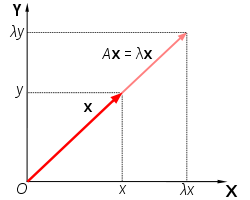
\includegraphics[scale=0.8]{Eigenvectors.png}
\end{center}

\section{Diagonalisation}

\begin{definition}
An $n\times n$ matrix $A$ over $\K$ is \emph{diagonalisable} if there exists an invertible matrix $P$ such
that $P^{-1}\cdot A\cdot P$ is a diagonal matrix.
\end{definition}

\begin{theorem}
An $n\times n$ matrix $A$ over $\K$ is diagonalisable if and only if $\K^n$ has a basis
$\{\vv_1,\ldots,\vv_n\}$ consisting of eigenvectors of $A$. In that case one may take
$P = (\vv_1\ \vv_2\ \ldots\ \vv_n)$, the matrix with the eigenvectors as columns, and then
\[
P^{-1}\, A\, P = \left( \begin{array}{cccc}
\lambda_1 & 0 & \ldots & 0\\ 0 & \lambda_2 & \ldots & 0\\ \vdots & \vdots & \ddots & \vdots\\ 0 & 0 & \ldots & \lambda_n
\end{array} \right) =: D,
\]
where $\lambda_i$ is the eigenvalue corresponding to the eigenvector $\vv_i$.
\end{theorem}

\begin{remark}
In the language of Chapter~\ref{ch:linear-mappings}: $P$ is the change-of-basis matrix from the
eigenvector basis to the standard basis, and $D = P^{-1}AP$ is the matrix of the operator
$\vv\mapsto A\vv$ written in the eigenvector basis. ``Diagonalisable'' therefore means ``similar to a
diagonal matrix'', and the closing example of the previous chapter, with
$M_S(F) = \left( \begin{smallmatrix} 3 & 0\\ 0 & 1 \end{smallmatrix} \right)$, was secretly a
diagonalisation.
\end{remark}

\begin{corollary}
If an $n\times n$ matrix has $n$ distinct eigenvalues in $\K$, then it is diagonalisable (eigenvectors for
distinct eigenvalues are linearly independent, and $n$ linearly independent vectors form a basis of $\K^n$).
\end{corollary}

\begin{example}[Powers of a matrix]
Diagonalisation makes it easy to compute powers of a matrix: if $A = P D P^{-1}$, then the inner factors
cancel in pairs,
\[
A^k = (PDP^{-1})(PDP^{-1})\cdots (PDP^{-1}) = P\, D^k\, P^{-1},
\]
and the power $D^k$ of a diagonal matrix is computed entrywise on the diagonal. For
$A = \left( \begin{smallmatrix} 2 & 1\\ 1 & 2 \end{smallmatrix} \right)$ we found the eigenvalues $1$ and
$3$ with eigenvectors $(1,-1)^T$ and $(1,1)^T$, so
\[
P = \left( \begin{array}{cc} 1 & 1\\ -1 & 1 \end{array} \right), \qquad
D = \left( \begin{array}{cc} 1 & 0\\ 0 & 3 \end{array} \right), \qquad
P^{-1} = \frac12\left( \begin{array}{cc} 1 & -1\\ 1 & 1 \end{array} \right),
\]
and therefore, for every $k\in\N$,
\[
A^k = P \left( \begin{array}{cc} 1 & 0\\ 0 & 3^k \end{array} \right) P^{-1}
= \frac12 \left( \begin{array}{cc} 3^k+1 & 3^k-1\\ 3^k-1 & 3^k+1 \end{array} \right).
\]
For $k=1$ this indeed recovers $A$.
\end{example}

\begin{warning}
Not every matrix is diagonalisable, even over $\C$: for
$A = \left( \begin{smallmatrix} 1 & 1\\ 0 & 1 \end{smallmatrix} \right)$ the only eigenvalue is
$\lambda = 1$, and its eigenspace $W_1 = \Span{\{(1,0)^T\}}$ is one-dimensional — there is no basis of
$\C^2$ consisting of eigenvectors of $A$.
\end{warning}

\section{Application: PageRank}

Eigenvectors for the eigenvalue $\lambda=1$ underlie Google's original PageRank algorithm for ranking web
pages.

A \emph{web graph} models the web: web pages are nodes and links are directed edges (arrows). For example:
\[
\begin{tikzcd}[row sep=large, column sep=large]
1 \arrow[r] & 2 \\
3 \arrow[u]\arrow[ur] & 4 \arrow[ul]\arrow[l]\arrow[u]
\end{tikzcd}
\]

\begin{definition}
In a web graph $G$, for a vertex $v$ let $l_v$ denote the number of outgoing edges starting at $v$.
\end{definition}

\noindent In the example above $l_1=1,\ l_2=0,\ l_3=2,\ l_4=3$.

\begin{definition}
For a web graph $G$ define its \emph{stochastic matrix} $S$ whose $ij$-entry is
\[
s_{ij} = \frac{1}{l_i} \quad\text{whenever there is a link from $i$ to $j$,} \qquad s_{ij}=0 \text{ otherwise.}
\]
If $l_i=0$, we set $s_{ii}=1$.
\end{definition}

\noindent For the graph above,
\[
S=\left( \begin{array}{cccc}
0 & 1 & 0 & 0\\
0 & 1 & 0 & 0\\
\tfrac{1}{2} & \tfrac{1}{2} & 0 & 0\\
\tfrac{1}{3} & \tfrac{1}{3} & \tfrac{1}{3} & 0
\end{array} \right).
\]

\begin{fact}
For the stochastic matrix $S$ of a web graph $G$:
\begin{itemize}
\item $0\leq s_{ij} \leq 1$ for all $i,j$;
\item $S\cdot (1,\ldots,1)^T = (1,\ldots,1)^T$;
\item $\lambda = 1$ is an eigenvalue of $S$ (and of $S^T$).
\end{itemize}
\end{fact}

Let $w$ be the vector whose $i$-th entry is the probability that a surfer visits web page $i$. Then $w$
satisfies
\[
S^T w = w, \qquad w \text{ has non-negative entries}, \qquad \text{the entries of } w \text{ sum to } 1.
\]

\begin{remark}
In general $S^T$ may have many eigenvectors for $\lambda=1$ satisfying these properties, so the ranking is not
yet well defined. This is fixed by the Google matrix below.
\end{remark}

\begin{definition}[Google matrix]
Let $\alpha$ be the \emph{damping factor} (e.g.\ $\alpha=0.85$) and let $v$ be a \emph{personalization
vector} with non-negative entries summing to $1$. Put
\[
G = \alpha \cdot S + (1-\alpha) \cdot (1,\ldots,1)^T \cdot v^T.
\]
The term $(1-\alpha)\,(1,\ldots,1)^T v^T$ models teleportation (random jumps).
\end{definition}

\begin{fact}
The matrix $G^T$ has a \emph{unique} eigenvector $\pi$ for $\lambda =1$ (that is, $G^T\pi=\pi$) whose entries
are non-negative and sum to $1$. The $i$-th entry of $\pi$ is the \emph{PageRank} of web page $i$.
\end{fact}


\renewcommand{\thechapter}{E}
\chapter{Exercises}\label{ch:exercises}
The exercises below come from the ten tutorial series accompanying the course (by A.~Pilitowska and
T.~Brengos), collected here in the notation of this book; the three complex-numbers series are merged
into a single section. Exercises marked with ($\ast$) are more challenging.

\clearpage
\section{Operations modulo \texorpdfstring{$n$}{n}. Groups and fields}

\begin{exercise}
Let $n$ be a fixed positive integer and let $a$ and $b$ be any two integers. Recall that $a$ is congruent
to $b$ modulo $n$ if $n$ divides $a-b$. Calculate:
\begin{enumerate*}[label=\alph*), itemjoin={\qquad}]
\item $17 \bmod 4$
\item $4 \bmod 17$
\item $(-2) \bmod 5$
\end{enumerate*}
\end{exercise}

\begin{exercise}
Solve the equations:
\begin{enumerate}[label=\alph*)]
\item $2x \equiv 1 \pmod 7$
\item $2x \equiv 1 \pmod 6$
\item $5x \equiv 1 \pmod 9$
\item $x^2 \equiv 3 \pmod{11}$
\item $2x+3 \equiv 0 \pmod 5$
\item $x+k \equiv 0 \pmod n$
\end{enumerate}
\end{exercise}

\begin{exercise}[$\ast$]
Prove that for all $n,k,p\in \Z$ we have the following:
\begin{enumerate}[label=\alph*)]
\item $(n \bmod k) \bmod k = n \bmod k$
\item $(n+p) \bmod k = \big((n \bmod k) + (p \bmod k)\big) \bmod k$
\item $(np) \bmod k = \big((n \bmod k)\,(p \bmod k)\big) \bmod k$
\end{enumerate}
\end{exercise}

\begin{exercise}
Recall that for $a,b\in\N$ the operations of addition and multiplication modulo $n$ are defined by
$a +_n b = (a+b) \bmod n$ and $a \cdot_n b = (a\cdot b) \bmod n$. Prove that:
\begin{enumerate}[label=\alph*)]
\item addition modulo $n$ is associative, i.e.\ $(a +_n b) +_n c = a +_n (b +_n c)$ for any $a,b,c\in\N$;
\item multiplication modulo $n$ is associative, i.e.\ $(a \cdot_n b) \cdot_n c = a \cdot_n (b \cdot_n c)$
for any $a,b,c\in\N$;
\item multiplication modulo $n$ is distributive with respect to addition modulo $n$, i.e.\
$(a +_n b) \cdot_n c = (a \cdot_n c) +_n (b \cdot_n c)$ for any $a,b,c\in\N$.
\end{enumerate}
\end{exercise}

\begin{exercise}
State which of the following are groups:
\begin{enumerate*}[label=\alph*), itemjoin={\qquad}]
\item $(\Z_n, +_n)$
\item $(\Z_n\setminus\{0\}, \cdot_n)$
\item $(\{1,2,3,4,6,12\}, \gcd)$
\end{enumerate*}
\end{exercise}

\begin{exercise}[$\ast$]
Show that $(2^X, \bigtriangleup)$ is a group, where $\bigtriangleup$ denotes the symmetric difference.
Construct the group table of $(2^{\{a,b,c\}}, \bigtriangleup)$.
\end{exercise}

\begin{exercise}
Show that $(\Z_n\setminus\{0\}, \cdot_n)$ is a group if and only if $n$ is a prime number.
\end{exercise}

\begin{exercise}
Verify whether $(\R_+, \bullet)$ is a group, where $a\bullet b = a^2 b^2$.
\end{exercise}

\begin{exercise}
Let $p\in\N$ be a prime number. Show that $(\Z_p, +_p, \cdot_p)$ is a field.
\end{exercise}

\begin{exercise}
Determine which of the following structures are fields. Do this in two steps: first verify whether the
set is a group with respect to the first operation, and then whether the set without the identity element
of the first operation is a group with respect to the second operation. Here $2^X$ carries the operations
$\cup$, $\cap$ and the symmetric difference $\bigtriangleup$, while $\R^\R$ denotes the set of all
functions $\R\to\R$, with pointwise addition $+$ and composition $\circ$.
\begin{enumerate*}[label=\alph*), itemjoin={\qquad}]
\item $(2^X, \cup, \cap)$
\item $(\R^\R, +, \circ)$
\item $(2^X, \cap, \cup)$
\item $(\R^\R, \circ, +)$
\item $(2^X, \cap, \bigtriangleup)$
\item $(2^X, \bigtriangleup, \cap)$
\item $(2^X, \cup, \bigtriangleup)$
\item $(2^X, \bigtriangleup, \cup)$
\end{enumerate*}
\end{exercise}

\begin{exercise}
Verify whether $(\R, \oplus, \odot)$ is a field, where $a \oplus b = a+b+1$ and $a\odot b = ab+a+b$.
\end{exercise}

\clearpage
\section{Complex numbers}

\begin{exercise}
Calculate:
\begin{enumerate*}[label=\alph*), itemjoin={\qquad}]
\item $(2+3i)(4-2i)$
\item $(1+2i)(2i-1)$
\item $(3+i)(3-i)$
\item $(a+bi)(a-bi)$
\end{enumerate*}
\end{exercise}

\begin{exercise}
Calculate:
\begin{enumerate*}[label=\alph*), itemjoin={\qquad}]
\item $\dfrac{2-3i}{3+4i}$
\item $\dfrac{i}{1+i}$
\item $\dfrac{3-4i}{i}$
\end{enumerate*}
\end{exercise}

\begin{exercise}
Calculate:
\begin{enumerate*}[label=\alph*), itemjoin={\qquad}]
\item $\dfrac{1+4i}{4-i}$
\item $\dfrac{(3+4i)^4}{(3-4i)^3}$
\end{enumerate*}
\end{exercise}

\begin{exercise}
Show that for every two complex numbers $z$ and $w$:
\begin{enumerate}[label=\alph*)]
\item $\overline{z+w} = \bar z + \bar w$ and $\overline{zw} = \bar z\, \bar w$
\item $|zw| = |z|\,|w|$
\item $\left|\dfrac{z}{w}\right| = \dfrac{|z|}{|w|}$
\end{enumerate}
\end{exercise}

\begin{exercise}[$\ast$]
Show that multiplication of complex numbers is associative.
\end{exercise}

\begin{exercise}[$\ast$]
Show that multiplication of complex numbers is distributive with respect to addition.
\end{exercise}

\begin{exercise}
Describe geometrically the sets of points $z\in\C$ satisfying the following conditions:
\begin{multicols}{2}
\begin{enumerate}[label=\alph*)]
\item $|z-i+3| = 5$
\item $|z-i+3| > 5$
\item $|z-1+3i| \leq 5$
\item $2\leq |z+i| < 4$
\item $\Re\big((z-i)^2\big) = 0$
\item $\Re(z^2) = 2$ and $\big(\Im(z+i)\big)^2 = 1$
\item $\left|\dfrac{z+3}{z-2i}\right| \geq 1$
\item $\Re(z+1)<0$ and $|i-z|\leq 3$
\end{enumerate}
\end{multicols}
\end{exercise}

\begin{exercise}
State which of the following are groups:
\begin{enumerate*}[label=\alph*), itemjoin={\qquad}]
\item $(\{z\in\C \mid |z|=1\}, +)$
\item $(\{z\in\C \mid |z|=1\}, \cdot)$
\end{enumerate*}
\end{exercise}

\begin{exercise}
Find polar forms of the following complex numbers:
\begin{multicols}{2}
\begin{enumerate}[label=\alph*)]
\item $1+i$
\item $-3$ (negative $3$)
\item $-i$
\item $2+2i$
\item $3+3\sqrt3\, i$
\item $z = \sin\alpha + i\cos\alpha$
\item $1 - i\sqrt3$
\item $-z$, if $z = \cos\alpha + i \sin\alpha$
\item $\sqrt3 - i$
\item $\bar z$, if $z = \cos\alpha + i \sin\alpha$
\item $\tfrac12 + \tfrac{\sqrt3}{2}\, i$
\end{enumerate}
\end{multicols}
\end{exercise}

\begin{exercise}
Calculate:
\begin{multicols}{2}
\begin{enumerate}[label=\alph*)]
\item $\sqrt[3]{(1+i)^6}$
\item $\left(\dfrac{1-i}{1+i}\right)^{222}$
\item $\left(\dfrac12 + i\,\dfrac{\sqrt3}{2}\right)^{124}$
\item $\left(\dfrac{2+2i}{\sqrt3 - i}\right)^{8}$
\item $\sqrt[6]{1}$
\item $\sqrt[4]{-1}$
\item $\sqrt[4]{(3-5i)^4}$
\item $\sqrt[6]{-1}$
\end{enumerate}
\end{multicols}
\end{exercise}

\begin{exercise}
Describe geometrically the sets of all the following roots:
\begin{enumerate*}[label=\alph*), itemjoin={\qquad}]
\item $\sqrt[6]{1}$
\item $\sqrt[4]{-1}$
\item $\sqrt[8]{1}$
\item $\sqrt[6]{-1}$
\end{enumerate*}
\end{exercise}

\begin{exercise}
Show that for every $n$ all complex roots of $1$ of order $n$ form a group under multiplication. Write
down the table of the group of all complex roots of $1$ of order $4$.
\end{exercise}

\begin{exercise}
Use De Moivre's formula to:
\begin{enumerate}[label=(\alph*)]
\item express $\sin 5\alpha$ in terms of $\sin\alpha$ and $\cos\alpha$,
\item express $\cos 4\alpha$ in terms of $\sin\alpha$ and $\cos\alpha$.
\end{enumerate}
\end{exercise}

\begin{exercise}[$\ast$]
Prove that
\[
\frac{\cos\alpha + i \sin\alpha}{\cos\beta + i\sin\beta} = \cos(\alpha-\beta) + i \sin(\alpha - \beta).
\]
\end{exercise}

\begin{exercise}
Find the polar form of:
\begin{enumerate*}[label=\alph*), itemjoin={\qquad}]
\item $2+\sqrt2 + i \sqrt 2$
\item $2 + i + i\sqrt3$
\end{enumerate*}
\end{exercise}

\begin{exercise}
Calculate:
\begin{enumerate*}[label=\alph*), itemjoin={\qquad}]
\item $\cos\tfrac{\pi}{12}$
\item $\cos 105^\circ$
\item $\cos 75^\circ$
\item $\cos(-15^\circ)$
\end{enumerate*}
\end{exercise}

\begin{exercise}[$\ast$]
Calculate $(1+\cos\alpha+i\sin\alpha)^{10}$ for $\alpha\in [0,\pi)$.
\end{exercise}

\begin{exercise}
Let $f(x)\in\R[x]$. Show that $z$ is a root of $f$ if and only if $\bar z$ is a root of $f$.
\end{exercise}

\begin{exercise}
Factor each of the following polynomials into a product of factors of degree at most $2$:
\begin{enumerate*}[label=\alph*), itemjoin={\qquad}]
\item $x^6+1$
\item $x^4+1$
\item $x^6+x^3+1$
\item $x^5+1$
\end{enumerate*}
\end{exercise}

\begin{exercise}
Prove that every polynomial of an odd degree, with all real coefficients, has at least one real root.
\end{exercise}

\begin{exercise}
Knowing that $1-2i$ is a root of the polynomial $z^4+2z^3+2z^2+10z+25$, find all remaining roots.
\end{exercise}

\begin{exercise}
Knowing that $2+i$ is a root of the polynomial $z^4-2z^3-6z^2+22z-15$, find all remaining roots.
\end{exercise}

\begin{exercise}
Solve the equations:
\begin{enumerate*}[label=\alph*), itemjoin={\qquad}]
\item $x^2+x+1 = 0$
\item $2x^2+ix+3 = 0$
\item $x^2+2x-i\sqrt3 = 0$
\end{enumerate*}
\end{exercise}

\clearpage
\section{Vector spaces}

\begin{exercise}
Determine whether or not the following sets are vector spaces over the indicated fields:
\begin{enumerate}[label=(\alph*)]
\item $\Z$ over $\Z_2$, with addition of integers, and scaling defined as $0\cdot z = 0$, $1\cdot z = z$
for every $z\in\Z$
\item $\Z_4$ over $\Z_2$, with addition modulo $4$, and scaling defined as $0\cdot z = 0$,
$1\cdot z = z$ for every $z\in\Z_4$
\item $\C$ over $\R$, with addition of complex numbers, and scaling by real numbers
\item $\R$ over $\C$, with addition of real numbers, and scaling by complex numbers
\item all subsets of a finite set $X$ over $\Z_2$, with the symmetric difference as vector addition, and
with scaling defined as $0\cdot A = \emptyset$ and $1\cdot A = A$ for every $A\subseteq X$
\item $\R_+$ over $\R$, with addition of real numbers, and scaling defined as $p\odot r = r^p$ for every
$r\in\R_+$ and $p\in\R$
\end{enumerate}
\end{exercise}

\begin{exercise}
Decide which of the following subsets are subspaces:
\begin{enumerate}[label=(\alph*)]
\item $\{(x,y)\in\R^2 \mid x\geq 0,\ y\geq 0\}\subseteq \R^2$
\item $\{(x,y,z)\in\R^3 \mid yz \leq 0\}\subseteq \R^3$
\item $\{(x,y,z)\in\R^3 \mid x+y+z = x-y = 0\}\subseteq \R^3$
\item $\{(x,y)\in\R^2 \mid |x-y|\leq 1\}\subseteq \R^2$
\end{enumerate}
\end{exercise}

\begin{exercise}[$\ast$]
Prove that in a vector space $\V$ over a field $\K$, for every $\vv,\uu\in \V$ and $\lambda\in\K$,
\[
\lambda\cdot(\vv-\uu) = \lambda\cdot\vv - \lambda\cdot\uu.
\]
\end{exercise}

\begin{exercise}
The intersection of any collection of subspaces of a vector space $\V$ is a subspace of $\V$. Show that
this is not necessarily true for the union of subspaces.
\end{exercise}

\begin{exercise}
The real plane $\R^2$ is a vector space over $\R$. Describe, in geometrical terms, all subspaces of
$\R^2$.
\end{exercise}

\begin{exercise}[$\ast$]
Let $\V$ be a vector space over a field $\K$ and let $S,T\subseteq \V$. Prove that:
\begin{enumerate}[label=(\alph*)]
\item $S\subseteq \Span{S}$
\item $S\subseteq T \implies \Span{S}\subseteq\Span{T}$
\item $\Span{\Span{S}} = \Span{S}$
\item $\vv\in\Span{S} \iff \Span{S} = \Span{S\cup\{\vv\}}$.
\end{enumerate}
\end{exercise}

\clearpage
\section{Linear independence. Bases and dimension}

\begin{exercise}
Decide whether the given sequence of vectors is linearly independent in the indicated vector space:
\begin{enumerate}[label=(\alph*)]
\item $\big((1,0,1),(1,1,0),(0,1,1)\big)$ in $\R^3$ over $\R$
\item $\big((1,0,1),(1,1,0),(0,1,1)\big)$ in $\Z_2^3$ over $\Z_2$
\end{enumerate}
\end{exercise}

\begin{exercise}
Let $\V$ be any vector space over a field $\K$ and let $\vv_1,\vv_2,\ldots,\vv_n,\uu \in \V$. Decide
whether the given sequence of vectors is linearly independent:
\begin{enumerate}[label=(\alph*)]
\item $(\vv_1,\ \vv_1+\vv_2,\ \vv_1+\vv_2+\vv_3,\ \ldots,\ \vv_1+\ldots+\vv_{n-1}+\vv_n)$ if the sequence
$(\vv_1,\vv_2,\ldots,\vv_n)$ is linearly independent
\item $(\vv_1+\vv_2,\ \vv_2+\vv_3,\ \ldots,\ \vv_{n-1}+\vv_n,\ \vv_n+\vv_1)$ if the sequence
$(\vv_1,\vv_2,\ldots,\vv_n)$ is linearly independent
\item $(\vv_1+\uu,\ \vv_2+\uu,\ \ldots,\ \vv_n+\uu)$ if the sequence $(\vv_1,\vv_2,\ldots,\vv_n)$ is
linearly independent and $\uu\in \V$ is any vector
\item $S$, where $S$ is a subsequence of a linearly independent sequence $T$ of vectors from $\V$
\item $S$, where $S$ is a sequence of vectors from $\V$ containing a linearly independent subsequence $T$
\item ($\ast$) $(\vv_1,\vv_2,\ldots,\vv_n)$, where $\vv_i\in\Span{S_i}$ and $\vv_i\neq \0$ for
$i = 1,2,\ldots,n$, the sets $S_i\subseteq \V$ are finite and pairwise disjoint, and the set
$S_1\cup S_2\cup\ldots\cup S_n$ consists of linearly independent vectors.
\end{enumerate}
\end{exercise}

\begin{exercise}
Find the dimension of each of the following vector spaces:
\begin{enumerate}[label=(\alph*)]
\item $\C$ over $\R$
\item $\K^n$ over any field $\K$
\item $\Span{\{\vv_1,\vv_2,\ldots,\vv_{n-1}\}}$, where $(\vv_1,\vv_2,\ldots,\vv_n)$ is a basis of a
vector space $\V$ over a field $\K$
\item $\Span{\{\vv_n,\vv_{n-1},\ldots,\vv_1\}}$, where $(\vv_1,\vv_2,\ldots,\vv_n)$ is a basis of a
vector space $\V$ over a field $\K$
\item $\{(x,y,z,t)\in\R^4 \mid x+y+z+t = 0\}$
\item $\{(x,y,z,t)\in\R^4 \mid 2x+y = z-t\}$
\item $\Span{\{(1,2,1,0),(1,3,1,1),(0,1,2,-1),(-3,1,2,2)\}}$ over $\R$
\item $2^{\{a,b,c\}}$ over $\Z_2$ (with the symmetric difference as vector addition).
\end{enumerate}
\end{exercise}

\begin{exercise}
Calculate the coordinates of the vector $\vv$ with respect to the basis $S$:
\begin{enumerate}[label=(\alph*)]
\item $\vv = (1,2,3,4)$, $\ S = \big((1,1,1,1),(1,1,1,0),(1,1,0,1),(1,0,1,1)\big)$
\item $\vv = \{a,b\}$, $\ S = \big(\{a\},\{b\},\{c\}\big)$ in the vector space $2^{\{a,b,c\}}$ over
$\Z_2$
\item $\vv = \vv_1$, $\ S = (\vv_1,\vv_2,\ldots,\vv_n)$
\item $\vv = \vv_1+\vv_2+\ldots+\vv_n$, $\ S = (\vv_1,\vv_2,\ldots,\vv_n)$.
\end{enumerate}
\end{exercise}

\begin{exercise}[$\ast$]
Prove that if $(\vv_1,\vv_2,\ldots,\vv_n)$ is a basis of a vector space $\V$, then so is
$(\vv_1,\ \vv_1+\vv_2,\ \ldots,\ \vv_1+\vv_2+\ldots+\vv_n)$.
\end{exercise}

\begin{exercise}[$\ast$]
Prove that $\dim\Span{A\cup B} \leq \dim\Span{A} + \dim\Span{B}$ for subsets $A,B$ of a vector space
$\V$.
\end{exercise}

\clearpage
\section{Matrices}

\begin{exercise}
For the following matrices $A$ and $B$ calculate the matrix $A\cdot B$:
\begin{enumerate}[label=(\alph*)]
\item $A = \left( \begin{array}{cc} 1 & 0\\ 2 & 3\\ 1 & 2\\ -1 & 1 \end{array} \right)$, \quad
$B = \left( \begin{array}{ccc} 3 & -2 & 2\\ 1 & 5 & 3 \end{array} \right)$ \quad over the field $\R$
\item $A = \left( \begin{array}{ccc} 1 & 1 & 1\\ 1 & 1 & 1\\ 1 & 1 & 1 \end{array} \right)$, \quad
$B = \left( \begin{array}{ccc} 1 & 4 & 0\\ 2 & 5 & 1\\ 3 & 6 & 2 \end{array} \right)$ \quad over the
field $\Z_7$
\item $A = \left( \begin{array}{cccc} 1 & 1 & 0 & 0\\ 3 & 2 & 3 & 1\\ 1 & 0 & 1 & 0 \end{array} \right)$,
\quad $B = \left( \begin{array}{cc} 2 & 1\\ 1 & 0\\ 2 & 0\\ 1 & 1 \end{array} \right)$ \quad over the
field $\Z_5$
\end{enumerate}
\end{exercise}

\begin{exercise}
Recall that a square matrix $A$ is symmetric if and only if $A = A^T$. Is it true that multiplication of
symmetric matrices is commutative?
\end{exercise}

\begin{exercise}
Show for matrices $A$ and $B$ (of appropriate sizes) that $(A\cdot B)^T = B^T\cdot A^T$.
\end{exercise}

\begin{exercise}
Use matrices to determine the dimension of the subspace $W$ over the field $\R$:
\begin{enumerate}[label=(\alph*)]
\item $W = \Span{\{(1,2,3),(1,-1,2),(-1,4,-1)\}}$
\item $W = \Span{\{(3,1,2,1),(1,-1,1,2),(2,3,0,-3),(2,-1,1,2)\}}$
\end{enumerate}
\end{exercise}

\begin{exercise}
Calculate the following determinants:
\begin{enumerate}[label=(\alph*)]
\item $\det \left( \begin{array}{cccc}
1 & 2 & -2 & 1\\ -3 & 1 & 3 & 2\\ -1 & 2 & 4 & 2\\ 5 & -1 & 2 & 2
\end{array} \right)$, where the matrix belongs to $\R_4^4$
\item $\det \left( \begin{array}{cccc}
1 & 2 & 1 & 3\\ 2 & 1 & 2 & 1\\ 3 & 2 & 3 & 2\\ 4 & 3 & 4 & 3
\end{array} \right)$, where the matrix belongs to $(\Z_5)_4^4$
\item $\det(A)$, where $A\in \K_5^5$ has the entries $a_{ij} = i-j$.
\end{enumerate}
\end{exercise}

\begin{exercise}
The numbers $24026$, $40262$, $2624$, $26240$ and $62402$ are divisible by $41$. Prove that the following
determinant is also divisible by $41$:
\[
\det \left( \begin{array}{ccccc}
2 & 4 & 0 & 2 & 6\\
4 & 0 & 2 & 6 & 2\\
0 & 2 & 6 & 2 & 4\\
2 & 6 & 2 & 4 & 0\\
6 & 2 & 4 & 0 & 2
\end{array} \right).
\]
\end{exercise}

\begin{exercise}
Let $y\in\R$, $n\in\N$ and let $A\in\R_n^n$ be defined in the following way: $a_{ij} = y$ for
$j\neq n-i+1$ and $a_{ij} = 0$ for $j = n-i+1$. Find the determinant of $A$ for $n=3$, and then find the
general formula for the determinant of $A$ for an arbitrary $n\in\N$. Justify your answer.
\end{exercise}

\begin{exercise}
Show that for all matrices $A$ and $B$ of size $2\times 2$, $\ \det(A\cdot B) = \det(A)\cdot\det(B)$.
\end{exercise}

\begin{exercise}
Show, for invertible matrices $A$ and $B$, that $(A\cdot B)^{-1} = B^{-1}\cdot A^{-1}$.
\end{exercise}

\begin{exercise}
Calculate the inverse (if it exists) of each of the following matrices:
\[
A = \left( \begin{array}{cccc}
1 & 1 & 1 & 1\\ 0 & 1 & 1 & 1\\ 0 & 0 & 1 & 1\\ 0 & 0 & 0 & 1
\end{array} \right) \in (\Z_3)_4^4, \qquad
B = \left( \begin{array}{cccc}
1 & 2 & 2 & 1\\ 1 & 3 & 4 & 1\\ 0 & 3 & 1 & 0\\ 1 & 3 & 4 & 2
\end{array} \right) \in \R_4^4, \qquad
C = \left( \begin{array}{cccc}
1 & 2 & 2 & 1\\ 1 & 3 & 4 & 1\\ 0 & 3 & 1 & 0\\ 1 & 3 & 4 & 2
\end{array} \right) \in (\Z_5)_4^4.
\]
\end{exercise}

\clearpage
\section{Systems of linear equations}

\begin{exercise}
Find a basis and the dimension of the solution space over the field $\R$ of each of the following systems
of linear equations:
\[
\left\{ \begin{aligned}
x + 2y - 2z + 2s - t &= 0\\
x + 2y - z + 3s - 2t &= 0\\
2x + 4y - 7z + s + t &= 0
\end{aligned} \right.
\qquad\qquad
\left\{ \begin{aligned}
x + 2y - z + 3s - 4t &= 0\\
2x + 4y - 2z - s + 5t &= 0\\
2x + 4y - 2z + 4s - 2t &= 0
\end{aligned} \right.
\]
\end{exercise}

\begin{exercise}
Discuss the solvability of the following systems of equations over the field $\R$ in terms of the
parameters $a$ and $b$:
\[
\left\{ \begin{aligned}
ax + by + az + t &= 1\\
ax + y + az + t &= 1\\
x + y + az + at &= 1
\end{aligned} \right.
\qquad
\left\{ \begin{aligned}
x + 2y + 3z + 4t &= a\\
2x + 3y + 4z + 5t &= b\\
3x + 4y + 5z + 6t &= a\\
4x + 5y + 6z + 7t &= b
\end{aligned} \right.
\qquad
\left\{ \begin{aligned}
x + ay + az &= 1\\
ax + ay + z &= 1\\
ax + y + az &= 1\\
ax + ay + az &= 1
\end{aligned} \right.
\]
\end{exercise}

\begin{exercise}
Find general solutions of the following systems of equations over the field $\R$:
\begin{enumerate}[label=(\alph*)]
\item $\left\{ \begin{aligned}
2x + 2y + 3z + 4t &= 2\\
2x + 3y + 4z + 6t &= 0\\
3x + 4y + 5z + 6t &= 1\\
x + y + z + t &= 1
\end{aligned} \right.$
\item $\left\{ \begin{aligned}
x + y + z - t + u &= 1\\
x - y + z + t + u &= 1\\
-x + y - z + t - u &= 0
\end{aligned} \right.$
\item $\left\{ \begin{aligned}
x + y + z + t + u &= 0\\
x - 2y + 3z - 4t + 5u &= 0
\end{aligned} \right.$
\end{enumerate}
\end{exercise}

\begin{exercise}
Find all solutions in $\Z_7$ of the following system of equations:
\[
\left\{ \begin{aligned}
3x_1 + 4x_2 + 4x_3 + 6x_4 &= 1\\
4x_1 + 5x_2 + 4x_3 + x_4 &= 0\\
5x_1 + 6x_2 + 4x_3 + 3x_4 &= 6
\end{aligned} \right.
\qquad \text{over the field } \Z_7.
\]
\end{exercise}

\clearpage
\section{Linear mappings. Matrices of linear mappings}

\begin{exercise}
Verify which of the following mappings are linear:
\begin{enumerate}[label=(\alph*)]
\item $F\colon\R^3\to\R^2$, $\ F(x,y,z) = (x,\,z)$
\item $F\colon\R^2\to\R^2$, $\ F(x,y) = (3x+y+1,\ 2x-3y)$
\item $F\colon\R^2\to\R^3$, $\ F(x,y) = (x+2y,\ x-y,\ x)$
\item $F\colon\R\to\R$, $\ F(x) = |x|$
\item $F\colon\R^3\to\R^3$, $\ F(x,y,z) = (xy,\ x,\ z)$
\end{enumerate}
\end{exercise}

\begin{exercise}
Let $T\colon\C\to\C$, $\ T(z) = \bar z$.
\begin{enumerate}[label=(\alph*)]
\item Show that $T$ is \emph{not} linear if we consider $\C$ as a vector space over itself.
\item Show that $T$ is linear if we consider $\C$ as a vector space over $\R$.
\end{enumerate}
\end{exercise}

\begin{exercise}\label{ex:ker-im}
Find $\ker F$, $\operatorname{im} F$, $\rank(F)$ and the nullity of $F$ for the following linear mappings
$F\colon U\to V$:
\begin{enumerate}[label=(\alph*)]
\item $U = V = \R^3$, $\ F(x,y,z) = (x+y+z,\ x+y,\ x)$
\item $U = V = \R^3$, $\ F(x,y,z) = (x+y,\ x+y,\ x+2y-z)$
\item $U = \R^3$, $V = \R^2$, $\ F(x,y,z) = (x-y+z,\ x+y-z)$
\end{enumerate}
\end{exercise}

\begin{exercise}
Find the matrices of the linear mappings from Exercise~\ref{ex:ker-im} in the following bases of the
spaces $U$ and $V$, respectively:
\begin{enumerate}[label=(\alph*)]
\item the standard bases of unit vectors
\item $\big((1,1,1),(1,1,0),(1,0,0)\big)$ and $\big((1,0,0),(1,1,0),(1,1,1)\big)$
\item $\big((1,1,1),(1,0,0),(0,0,1)\big)$ and $\big((1,2),(3,3)\big)$
\end{enumerate}
\end{exercise}

\begin{exercise}
Find a formula and the matrix in the standard basis for the linear operator $F$ such that:
\begin{enumerate}[label=(\alph*)]
\item $F(1,1,1) = (1,0,1)$, $\ F(1,1,0) = F(0,1,1) = (1,1,1)$
\item $F(1,2,1) = (1,0,0)$, $\ F(1,0,1) = (0,1,0)$, $\ F(1,0,0) = (1,0,0)$
\item $F(1,0,0,0) = F(0,1,0,0) = F(0,0,1,0) = F(0,0,0,1) = (1,1,1,1)$
\end{enumerate}
\end{exercise}

\begin{exercise}\label{ex:matrix-bases}
Assuming that $A = M_S(F)$ is the matrix of a linear operator $F$ in the basis $S$, find the matrix
$B = M_R(F)$ of $F$ in the basis $R$:
\begin{enumerate}[label=(\alph*)]
\item $\left( \begin{array}{cc} 1 & 1\\ 1 & 2 \end{array} \right)$, for $S = \big((1,1),(1,2)\big)$ and
$R = \big((1,0),(0,1)\big)$
\item $\left( \begin{array}{ccc} 1 & 0 & 0\\ 0 & 1 & 0\\ 0 & 0 & 1 \end{array} \right)$, for
$S = \big((1,1,1),(0,1,2),(1,0,1)\big)$ and $R = \big((1,0,0),(0,1,0),(0,0,1)\big)$
\item $\left( \begin{array}{ccc} 1 & 2 & 2\\ 1 & 1 & 1\\ 2 & 0 & 0 \end{array} \right)$, for
$S = \big((1,1,1),(0,1,2),(1,0,1)\big)$ and $R = \big((1,0,0),(0,1,0),(0,0,1)\big)$
\item $\left( \begin{array}{cccc} 1 & 1 & 1 & 1\\ 0 & 1 & 1 & 1\\ 0 & 0 & 1 & 1\\ 0 & 0 & 0 & 1
\end{array} \right)$, for $S = \big((1,0,1,0),(0,0,1,1),(1,1,0,0),(1,0,1,1)\big)$ and\\
$R = \big((1,1,1,0),(1,1,0,1),(1,0,1,1),(0,1,1,1)\big)$
\end{enumerate}
\end{exercise}

\begin{exercise}
For each pair of matrices $A$ and $B$ from Exercise~\ref{ex:matrix-bases}, find a matrix $P$ such that
$A = P^{-1}\cdot B\cdot P$. Verify your solution by matrix multiplication.
\end{exercise}

\clearpage
\section{Eigenvalues and eigenvectors}

\begin{exercise}
Find the eigenvalues of $A = M_S(F)$:
\begin{enumerate}[label=(\alph*)]
\item $A = \left( \begin{array}{cc} 2+i & 1\\ 2 & 2-i \end{array} \right)$
\item $A = \left( \begin{array}{ccc} 2 & -1 & 2\\ 5 & -3 & 3\\ -1 & 0 & -2 \end{array} \right)$
\end{enumerate}
\end{exercise}

\begin{exercise}
Find all eigenvalues and a basis of each eigenspace for the following linear operators:
\begin{enumerate}[label=(\alph*)]
\item $F\colon\R^2\to\R^2$, $\ F(x,y) = (x,\ x+y)$
\item $F\colon\R^3\to\R^3$, $\ F(x,y,z) = (2x+y,\ y-z,\ 2y+4z)$
\item $F\colon\R^3\to\R^3$, $\ F(x,y,z) = (x-z,\ 2y,\ x+z)$
\item $F\colon\C^2\to\C^2$, $\ F(x,y) = (-y,\ x)$
\item $F\colon\C^3\to\C^3$, $\ F(x,y,z) = (x-z,\ 2y,\ x+z)$.
\end{enumerate}
\end{exercise}

\begin{exercise}\label{ex:eig-matrices}
Assuming that each of the following matrices represents a linear operator $F$ in a basis $S$, find all
eigenvectors and a basis of each eigenspace:
\begin{enumerate}[label=(\alph*)]
\item $A = M_S(F) = \left( \begin{array}{ccc} 3 & 1 & 1\\ 2 & 4 & 2\\ 1 & 3 & 3 \end{array} \right)$
\item $A = M_S(F) = \left( \begin{array}{ccc} 1 & 2 & 2\\ 1 & 2 & -1\\ -1 & 1 & 4 \end{array} \right)$
\item $A = M_S(F) = \left( \begin{array}{ccc} 1 & 1 & 0\\ 0 & 1 & 0\\ 0 & 0 & 1 \end{array} \right)$
\end{enumerate}
\end{exercise}

\begin{exercise}
For each operator $F$ from Exercise~\ref{ex:eig-matrices}, determine whether there exists a basis $T$
such that the matrix of the operator $F$ in the basis $T$ is diagonal.
\end{exercise}

\begin{exercise}
For the matrix
$A = \left( \begin{array}{ccc} 1 & 2 & -1\\ 1 & -1 & 0\\ 2 & -2 & 0 \end{array} \right)$
calculate $A^{100}$.
\end{exercise}

\begin{exercise}
For a linear mapping $F\colon\R^2\to\R^2$ such that $F(1,2) = (2,4)$ and $F(-2,1) = (-2,1)$, calculate
$F^{150}(1,0)$.
\end{exercise}


\end{document}
